% ! TEX root = ../../realeasythesis.tex  % jeffhere

\chapter{多個語音離散表徵與音位的關係}   \newcommand{\jefftablesep}{\vspace{0.5cm}}
\renewcommand{\arraystretch}{0.7}
\newcommand{\jcm}[1]{}


% \newcommand{\jefftablesep}{\vspace{0.5cm}}\renewcommand{\arraystretch}{0.7} % 調整行高

\section{動機} %%%

  如第三章所述,一個文字或音位往往對應到上百毫秒的語音訊號,然而單一離散單元所對應的聲音訊號為 10 或 20 毫秒,亦即同一段語音所對應的離散單元數目將比音位或文字多出許多。本章節從自然語言處理中獲取靈感,將文字處理中的分詞演算法(Tokenization)應用於離散單元序列上,使得離散單元重新組合成次詞單位(Subword Units),稱之為「聲學片段(Acoustic Piece)」,以這些由多個離散單元組成的符記(Token)\footnote{指資料序列中的離散基本單位。}作為新的基本單位重新編碼語音訊號,取代原先的離散單元。為了分析聲學片段的序列是否更接近音位的序列,在此將續用上一章節的分析方法,比對並檢驗引入次詞單位是否有機會得到更好的語音表徵,進而有機會用於無文字(Textless)架構\cite{lakhotia_generative_2021, lakhotia_generative_2021-1, noauthor_textless_2021}中。

\section{相關研究} 

  在無文字架構被提出後的約兩年後,藉助次詞單位組合離散單元的研究逐步出現。任氏(Ren)等人 \cite{ren_speech_2022}\citetag{1-22A4-Pretrain-ap})最先提出聲學片段的概念,該論文比對離散單元序列及對應的文字轉寫,從中觀察到許多相似的類型(Patterns)重複出現,而且不限於單一語者。受此啟發,本論文首先將離散單元,透過文字處理中常用以獲得次詞單位的「句片段(SentencePiece) \cite{kudo_sentencepiece_2018} 套件獲得新的符記 --- 「聲學片段」,並用於語音辨識的預訓練上。

        不久,由吳氏(Wu)提出的 Wav2seq \cite{wu_wav2seq_2023}\citetag{2-22A5-wav2seq}論文中,考量文字與語音的序列長度差異,並基於離散單元和音位的關聯性,將離散單元視為字符(Character),嘗試將這些字符透過次詞單位組成「虛擬語言(Pseudo-language\footnote{虛擬語言對應之離散單元被視為「虛擬文字(Pseudo-text)」})」,來幫助語音到文字的模型。在實際應用中,因為解碼器生成的目標文字序列亦是由次詞單位組成,因此該篇研究旨在讓模型在預訓練後可以快速適應下游任務。與前一篇呼應,聲學片段對語音預訓練的效果在\cite{10096788}\citetag{3-23A-coarser-grain}中被探討,此後聲學片段更被應用於縮短資料序列長度\cite{chang_exploration_2023}\citetag{4-23B-Exploration of Efficient End-to-End ASR using Discretized Input from Self-Supervised Learning} 、語音生成\cite{shen2024acoustic}\citetag{5-24A-speech-gen},或學習更穩健(Robust)的語音表徵\cite{chang2023r}\citetag{6-23B-rspin-acousticpiece}。

        近期,張氏(Chang)等人\cite{chang_exploring_2024}\citetag{7-23B-shinji-hsiuhsuan}將以分詞方法處理離散單元的流程(Pipeline)納入 ESPNet 套件 \cite{watanabe2018espnet} 中,並在語音辨識、語音翻譯等任務中獲得了超越以往的表現,進一步證明了這個方法的效果。

\section{文字處理中的分詞演算法}

  在以文字為主體的自然語言處理中,文字文本除了以單詞(Word)或字元(Character)為處理單位,更常見的作法是透過分詞演算法(Tokenization)將文本分段,以「次詞單位」構成詞彙表來重新編碼文本,用於文字模型的訓練與推理。

        使用次詞單位的優點包含:

\begin{enumerate}
    \item 固定詞彙表大小,避免未登錄詞(Out-of-vocabulary,OOV)。
    \item 縮短資料序列的長度,提升訓練和推論的效率。
    \item 分解單詞,捕捉更細緻的語意關係,模擬如英語中的字首(Prefix)、字尾(Suffix)等等具有特定意義的文字組合。
\end{enumerate}

\subsection{常見演算法}

  以下介紹幾種常見的分詞方法:

\paragraph{位元組對編碼(Byte Pair Encoding,BPE)} \hfill \break
%
  位元組對編碼 \cite{10.5555/177910.177914, sennrich_neural_2016} 是一種常用的分詞方法,最初來自資料壓縮技術 \cite{10.5555/177910.177914},後來被引入到自然語言處理領域,用以處理機器翻譯問題 \cite{sennrich_neural_2016} 。
該演算法從字元開始,根據詞彙表中各個次詞單位的頻率,反覆合併常見的字元成為新的次詞單位,直到達到預定的詞彙表大小。

\paragraph{單詞片段(WordPiece)} \hfill \break
%
  WordPiece \cite{wu2016google} 演算法由 Google 用以訓練機器翻譯系統,並在 BERT \cite{devlin_bert_2019} 模型中被使用而廣為人知。與位元組對編碼相似,同樣是透過反覆合併的策略,但合併的依據改以機率模型取代出現頻率。

\paragraph{單一詞語言模型(Unigram Language Model)} \hfill \break
%
  單一詞語言模型 \cite{kudo2018subword} 是基於語言模型的分詞方法,以機率分佈選擇次詞單位,並以最大化輸入文本的機率來為文本分段。

\subsection{「句片段(SentencePiece)」套件}

  「句片段(SentencePiece) \cite{kudo_sentencepiece_2018}
」是由 Google 開發的分詞套件,實作了前述的位元組對編碼和單一詞演算法。其優勢在於可應用於不同語言,尤其用於處理中文、日文等不使用空格分隔單詞的語言文本時,此套件大大的簡化了前處理的流程。
        考慮到語音訊號本身不如英語等文字,在書寫時就已經具備空格分隔單詞,因此本章節的所有次詞單位皆以句片段套件中的單一詞演算法取得。

\section{分析方式}

  本章節沿用上一章節 LibriSpeech 資料集的 train-clean-100 訓練子集,以單一詞演算法取得次詞單位,並嘗試 500、1000、8000、10000、20000 五種符記種數,對每一種語音表徵和 K-平均模型的分群數,各自取得五種聲學片段文本。

        比照第三章的分析方式,本章除了整體的純度與相互資訊數據外,亦同樣從聲學片段與音位的角度分別探討,藉由調整次詞單位的種類數量,探討引入次詞單位並改變符記數量,將如何影響這些符記序列與音位標註間的相關性。然而,為了避免結果呈現過於複雜,細部分析時將著重比對 500 和 1000 種次詞單位的結果變化。

        由於本章節探討重點為次詞單位種數變化的影響,延續第三章的發現,後續分析將以表現最好的 HuBERT 離散表徵為主。在需要比較離散單元分群數影響時,我們將比對分群數為 50 與 100 時的差異,否則為避免數據過於複雜,離散單元的分群數預設為 50 進行細部探討。

\section{分析結果} 

  承繼上一個章節的分析方法,我們先將純度等數據與條件機率熱圖 $p_{y|z}(i | j)$ \footnote{由於共同機率分佈熱圖 $p_{yz}$ 的數值對於觀察符記對應到音位的關係較不明顯,因此仿照 SpeechTokenizer \cite{zhang2024speechtokenizer}、DinoSR \cite{liu2024dinosr} 等論文使用 $p_{y|z}(i | j)$ 呈現。} 兩者互相對照,並以語音學排序呈現,觀察聲學片段與音位之間兩者的分佈關係。

\subsection{由聲學片段角度探討}
{
\subsubsection{聲學片段數量的影響}


{
\begin{table}[!htbp]
    \centering
    \begin{subtable}[t]{\textwidth}
        \centering
        \begin{tabular}{|c|c|c|c|c|c|} \hline 
                次詞單位種數& 音位純度 & 分群純度 & 音位熵 & 離散單元熵 &    PNMI \\ \hline 
離散單元& 0.5256& 0.3382& 3.3152& 3.8681& 0.4993\\ \hline 
                   500  &   0.5574   &  0.0829 &   3.3152  &  6.0282 & 0.5357 \\ \hline %%  1.7758       
                  1000  &   0.5744   &  0.0556 &   3.3152  &  6.6594 & 0.5466 \\ \hline %%  1.8120       
                  8000  &   0.5957   &  0.0257 &   3.3152  &  8.5192 & 0.5729 \\ \hline %%  1.8993       
                 10000  &   0.5955   &  0.0238 &   3.3152  &  8.7207 & 0.5750 \\ \hline %%  1.9063       
                 20000  &   0.5921   &  0.0182 &   3.3152  &  9.3527 & 0.5820 \\ \hline %%  1.9293       
        \end{tabular}
\caption{分群數 = 50}
        \label{tab:ch4-hubert-phn-clu050-}
    \end{subtable}        
    \jefftablesep        
    \begin{subtable}[t]{\textwidth}
        \centering
        \begin{tabular}{|c|c|c|c|c|c|} \hline 
                次詞單位種數& 音位純度 & 分群純度 & 音位熵 & 離散單元熵 &    PNMI \\ \hline 
離散單元& 0.6097& 0.2553& 3.3152& 4.5704& 0.5786\\ \hline 
                   500  &   0.6260   &  0.0972 &   3.3152  &  6.0655 & 0.5990 \\ \hline %%  1.9858       
                  1000  &   0.6372   &  0.0631 &   3.3152  &  6.7181 & 0.6089 \\ \hline %%  2.0186       
                  8000  &   0.6536   &  0.0237 &   3.3152  &  8.5954 & 0.6308 \\ \hline %%  2.0912       
                 10000  &   0.6527   &  0.0219 &   3.3152  &  8.7938 & 0.6324 \\ \hline %%  2.0965       
                 20000  &   0.6490   &  0.0173 &   3.3152  &  9.4123 & 0.6378 \\ \hline %%  2.1145       
        \end{tabular}
\caption{分群數 = 100}
        \label{tab:ch4-hubert-phn-clu100-}
    \end{subtable}        


\caption{HuBERT 模型在不同次詞單位種類數量時的純度分析數據}
    \label{tab:hubert-phn-results-}
\end{table}

}  % tables

{
    {
        \newcommand{\tempwidth}[0]{0.8\linewidth}
        \begin{figure}
             \centering
             \begin{subfigure}{\textwidth}
                 \centering
                 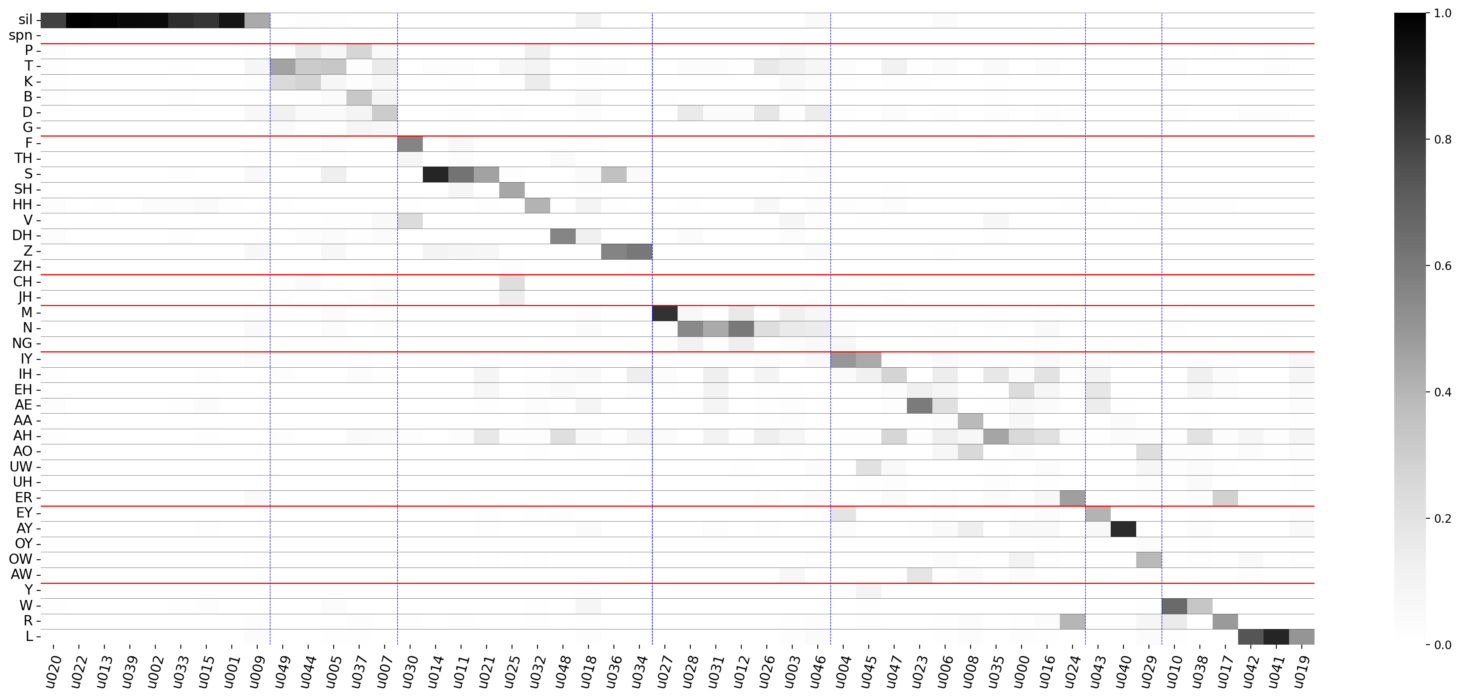
\includegraphics[width=\tempwidth]{figures/ch4figs/hub-u050-ap0000-givenunit-byphn.png}
                 \caption{離散單元}
                 \label{fig:hub-u050-ap0000-givenunit-byphn}
             \end{subfigure}
             \vfill
             \begin{subfigure}{\textwidth}
                 \centering
                 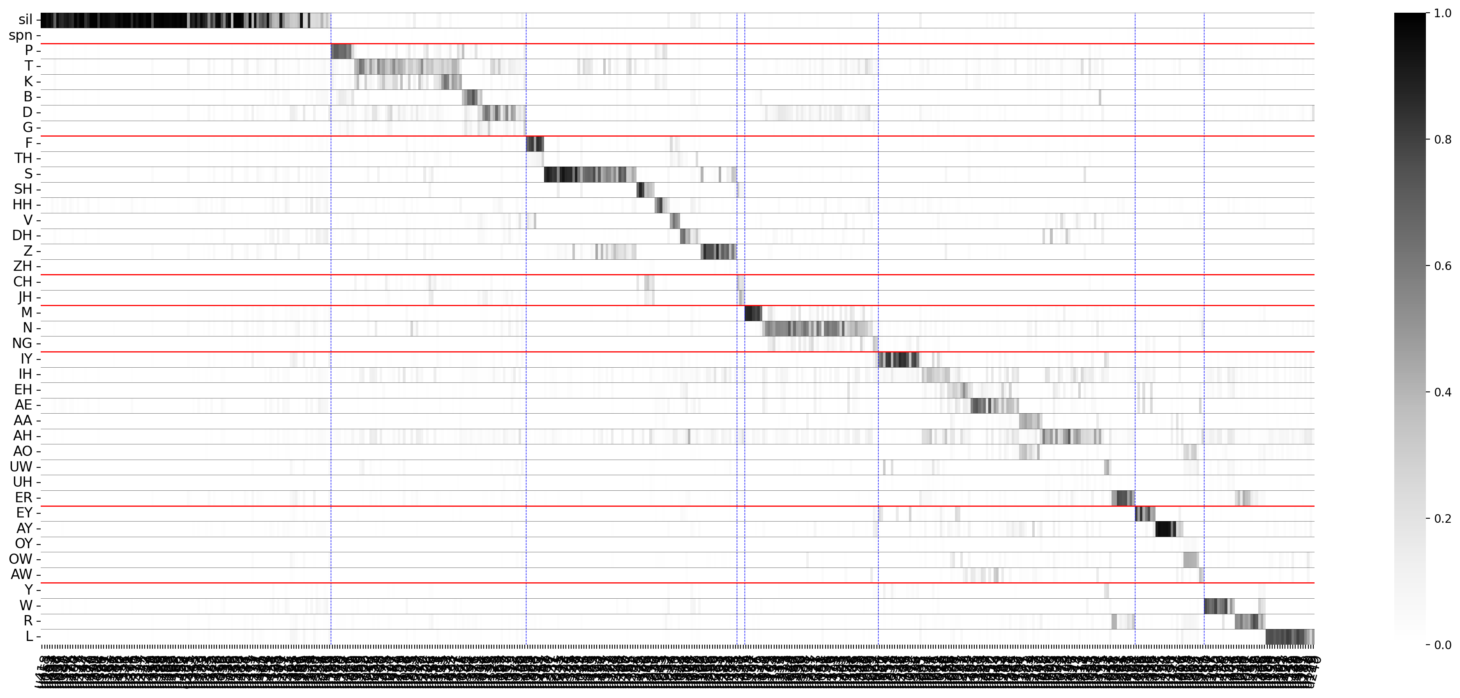
\includegraphics[width=\tempwidth]{figures/ch4figs/hub-u050-ap0500-givenunit-byphn.png}
                 \caption{500 種次詞單位}
                 \label{fig:hub-u050-ap0500-givenunit-byphn}
             \end{subfigure}
             \vfill
             \begin{subfigure}{\textwidth}
                 \centering
                 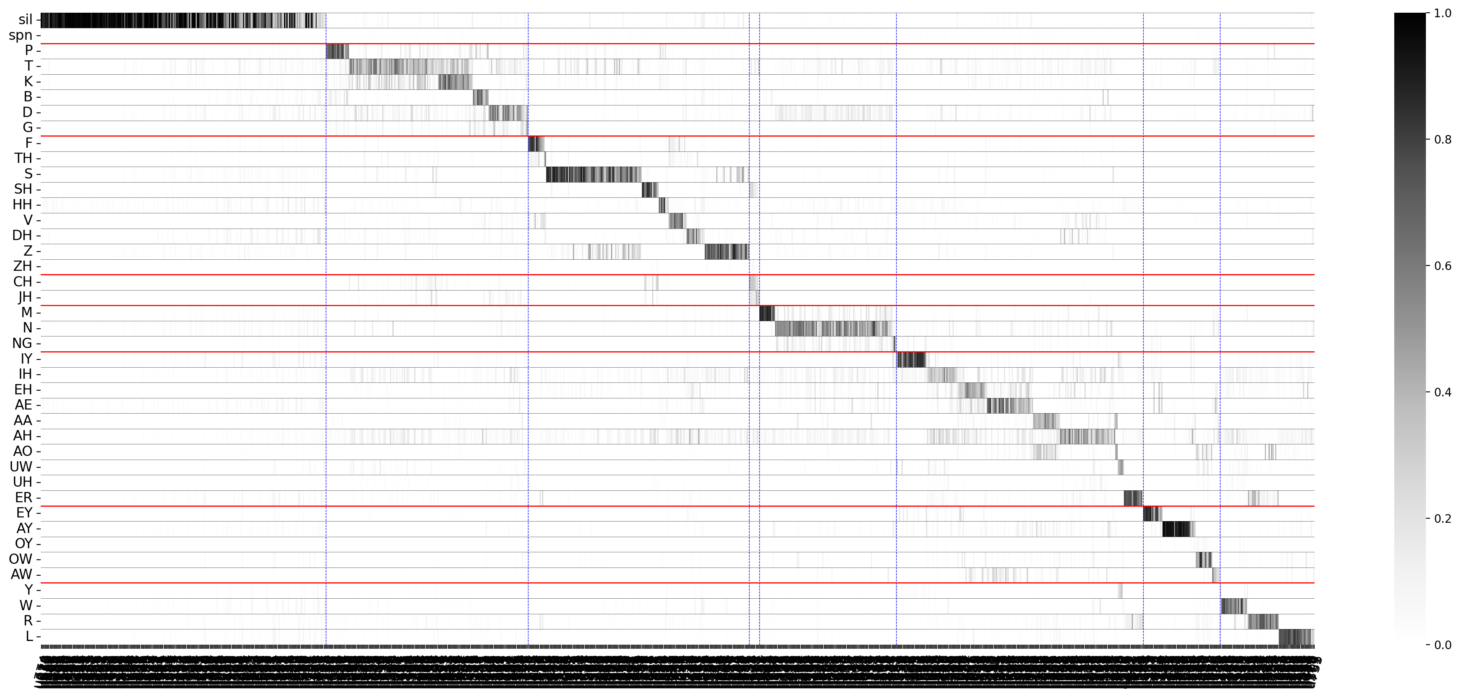
\includegraphics[width=\tempwidth]{figures/ch4figs/hub-u050-ap1000-givenunit-byphn.png}
                 \caption{1000 種次詞單位}
                 \label{fig:hub-u050-ap1000-givenunit-byphn}
             \end{subfigure}

             \caption{HuBERT 表徵在 K-平均演算法使用分群數 50 後,}
             比較不同次詞單位數量的條件機率分佈 $p_{y|z}(i | j)$ 熱圖
             \label{fig:hub-u050-comparisons}
        \end{figure}
    }
    {
        \newcommand{\tempwidth}[0]{0.8\linewidth}
        \begin{figure}
             \centering
             \begin{subfigure}{\textwidth}
                 \centering
                 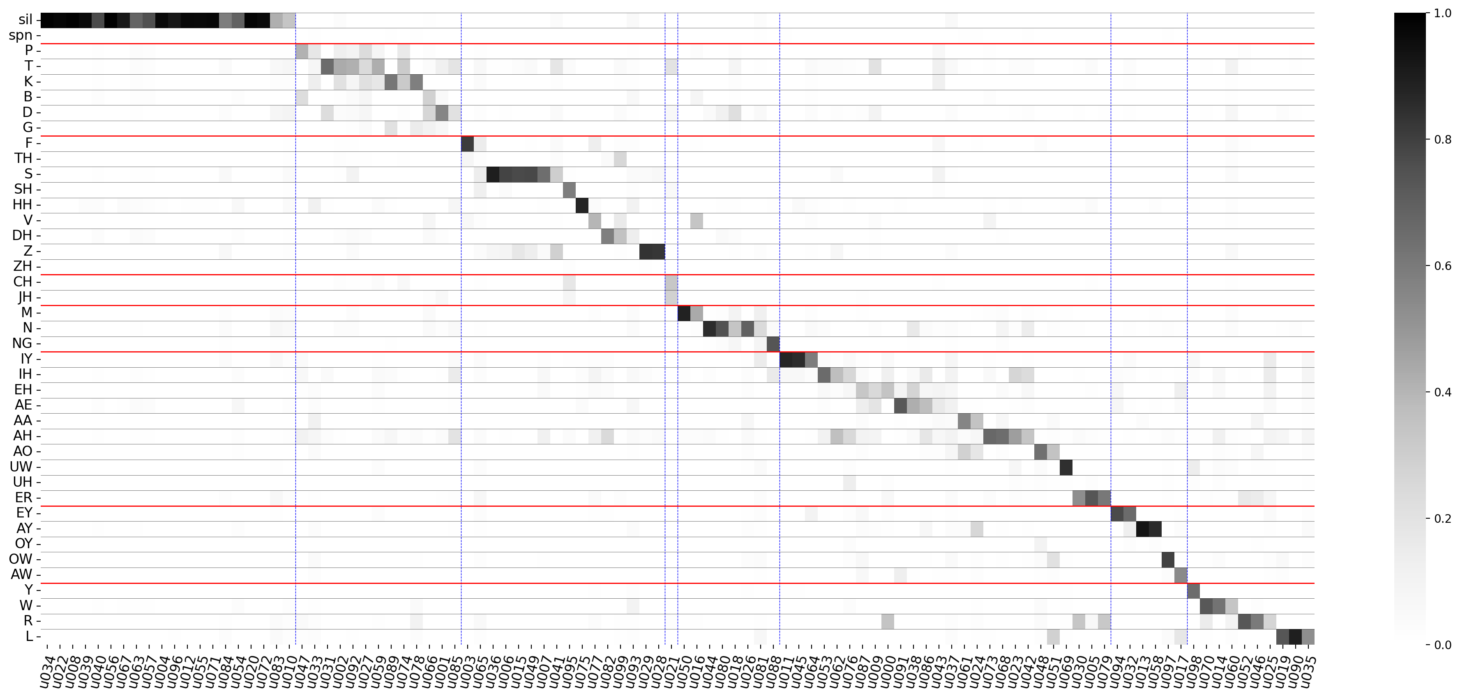
\includegraphics[width=\tempwidth]{figures/ch4figs/hub-u100-ap0000-givenunit-byphn.png}
                 \caption{離散單元}
                 \label{fig:hub-u100-ap0000-givenunit-byphn}
             \end{subfigure}
             \vfill
             \begin{subfigure}{\textwidth}
                 \centering
                 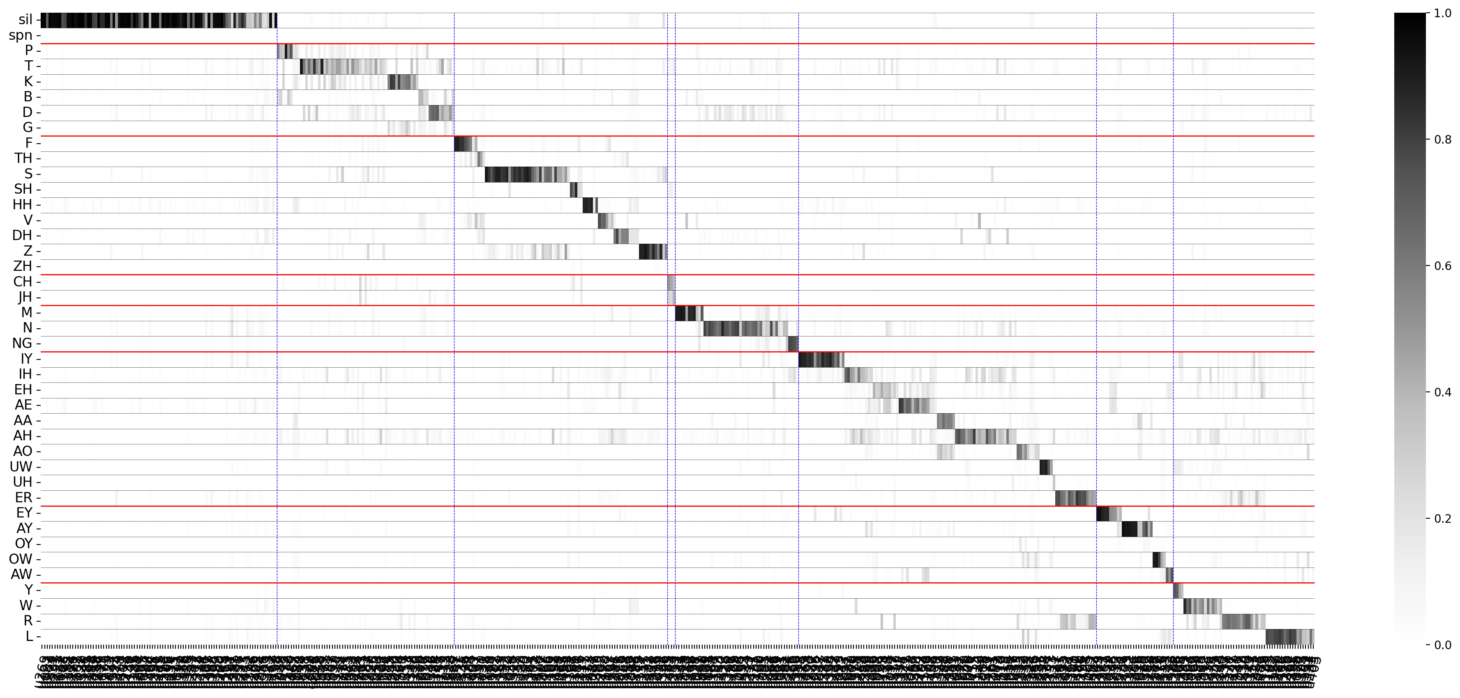
\includegraphics[width=\tempwidth]{figures/ch4figs/hub-u100-ap0500-givenunit-byphn.png}
                 \caption{500 種次詞單位}
                 \label{fig:hub-u100-ap0500-givenunit-byphn}
             \end{subfigure}
             \vfill
             \begin{subfigure}{\textwidth}
                 \centering
                 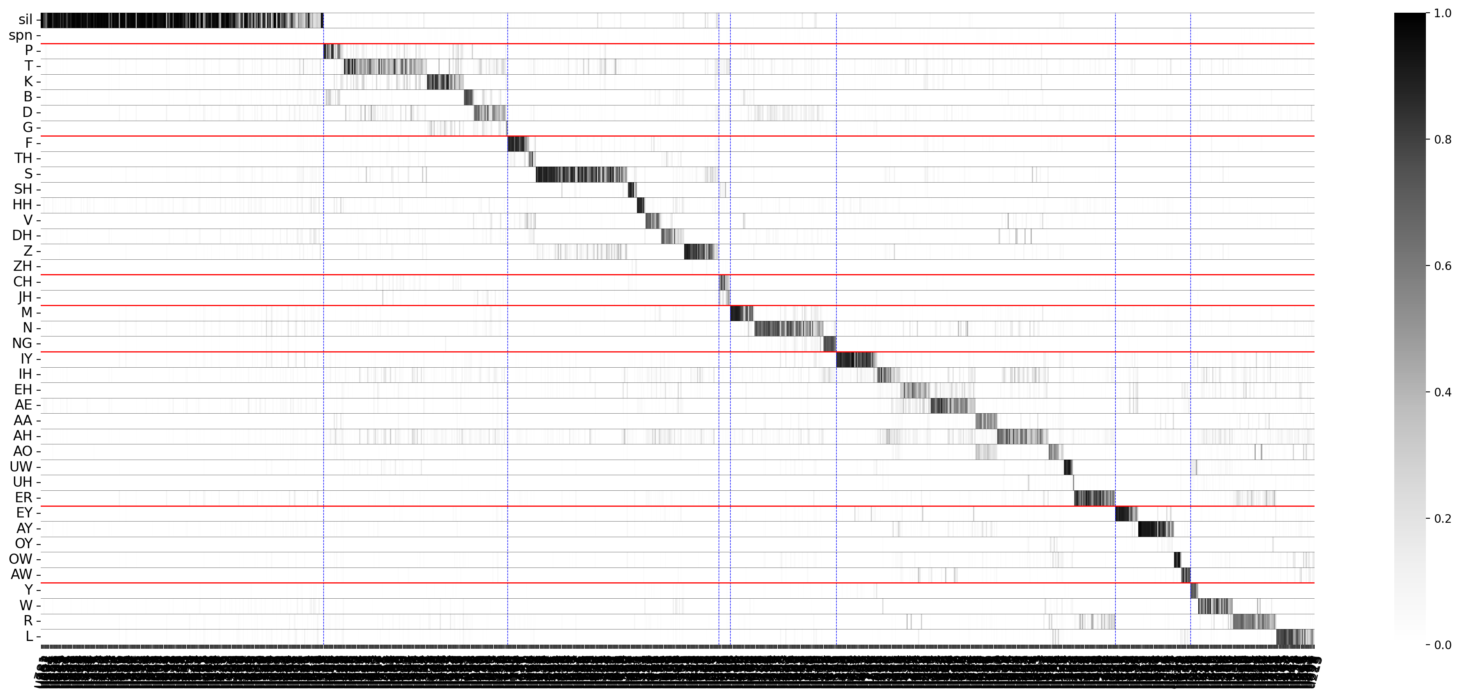
\includegraphics[width=\tempwidth]{figures/ch4figs/hub-u100-ap1000-givenunit-byphn.png}
                 \caption{1000 種次詞單位}
                 \label{fig:hub-u100-ap1000-givenunit-byphn}
             \end{subfigure}

             \caption{HuBERT 表徵在 K-平均演算法使用分群數 100 後,}
             比較不同次詞單位數量的條件機率分佈 $p_{y|z}(i | j)$ 熱圖
             \label{fig:hub-u100-comparisons}
        \end{figure}
    }
}

{
    {
        \newcommand{\tempwidth}[0]{0.7\linewidth}
        \begin{figure}
             \centering
             \begin{subfigure}{\textwidth}
                 \centering
                 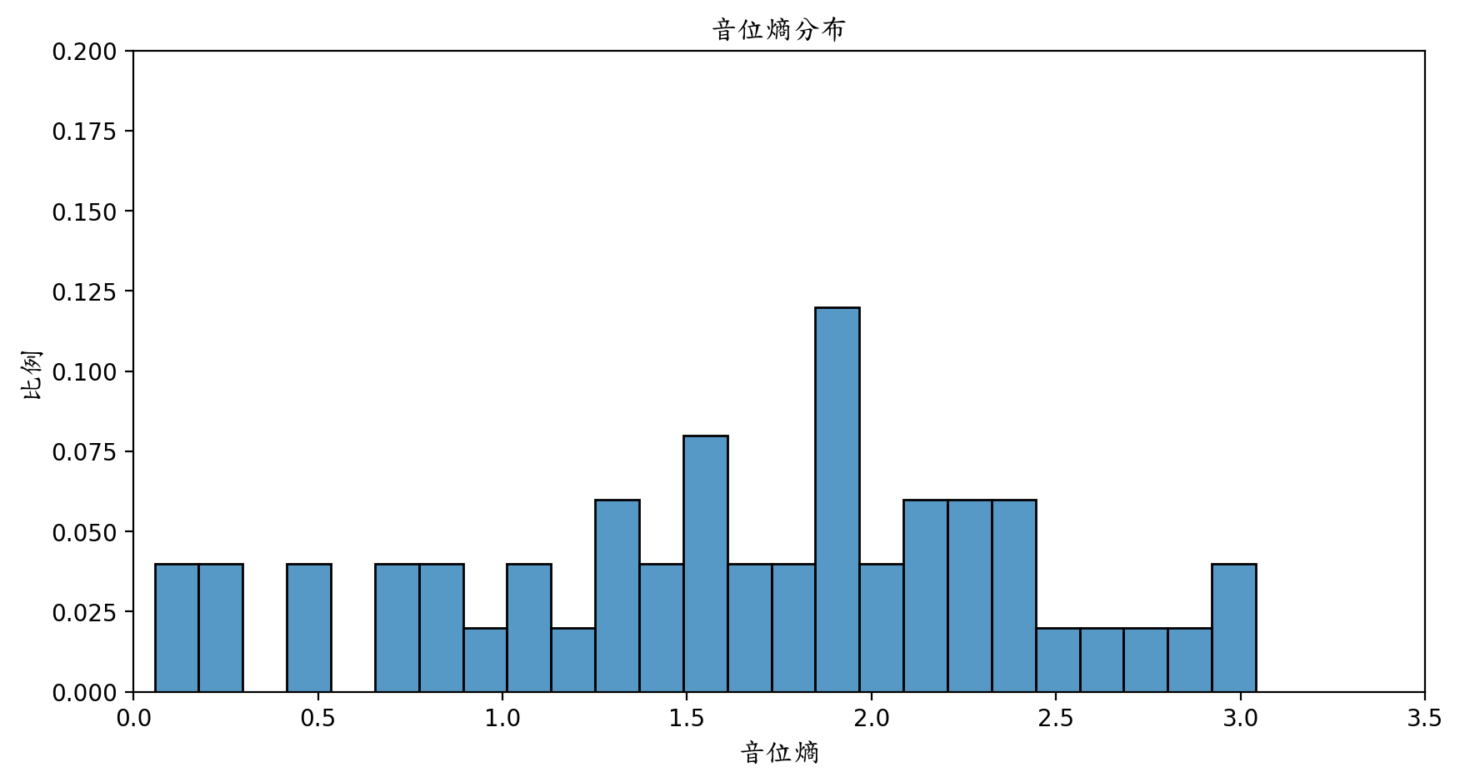
\includegraphics[width=\tempwidth]{figures/ch4figs/hub-u050-ap0000-phnent-hist.png}
                 \caption{離散單元}
                 \label{fig:hub-u050-ap0000-phnent-hist}
             \end{subfigure}
             \vfill
             \begin{subfigure}{\textwidth}
                 \centering
                 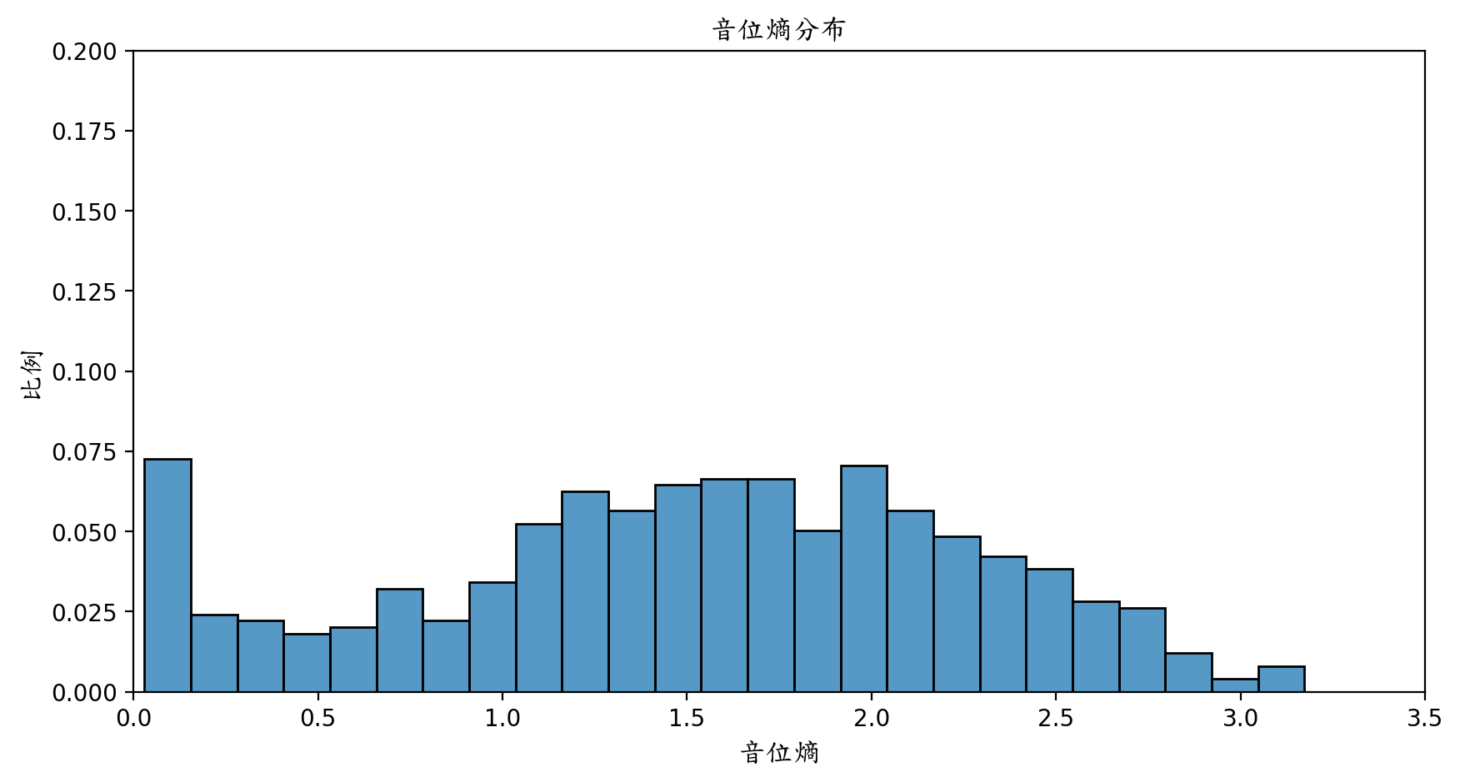
\includegraphics[width=\tempwidth]{figures/ch4figs/hub-u050-ap0500-phnent-hist.png}
                 \caption{500 種次詞單位}
                 \label{fig:hub-u050-ap0500-phnent-hist}
             \end{subfigure}
             \vfill
             \begin{subfigure}{\textwidth}
                 \centering
                 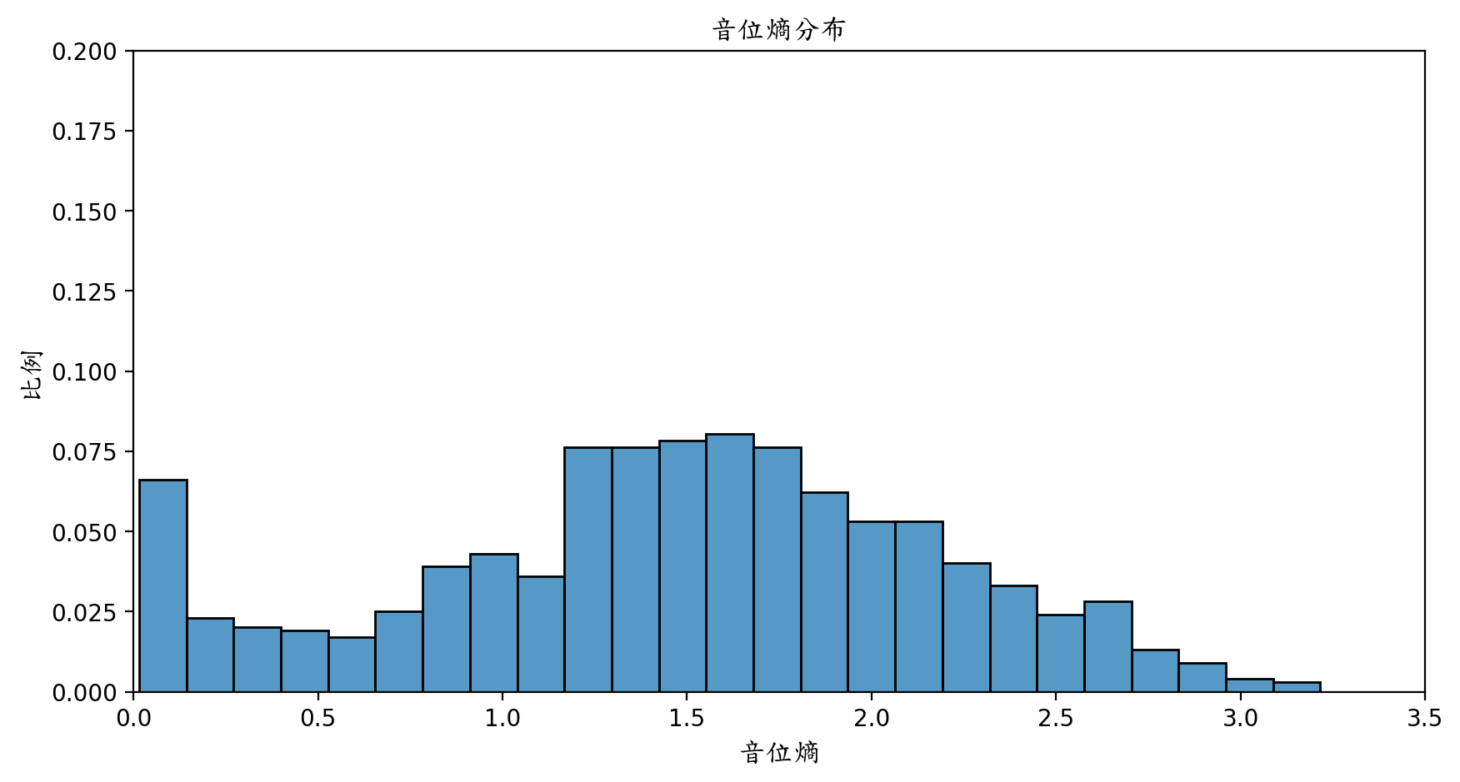
\includegraphics[width=\tempwidth]{figures/ch4figs/hub-u050-ap1000-phnent-hist.png}
                 \caption{1000 種次詞單位}
                 \label{fig:hub-u050-ap1000-phnent-hist}
             \end{subfigure}

             \caption{HuBERT 表徵在 K-平均演算法使用分群數 50 後,}
             比較不同次詞單位數量的音位條件熵 $H(y|z)$ 直方圖
             \label{fig:hub-u050-hist-comparisons}
        \end{figure}
    }
    {
        \newcommand{\tempwidth}[0]{0.7\linewidth}
        \begin{figure}
             \centering
             \begin{subfigure}{\textwidth}
                 \centering
                 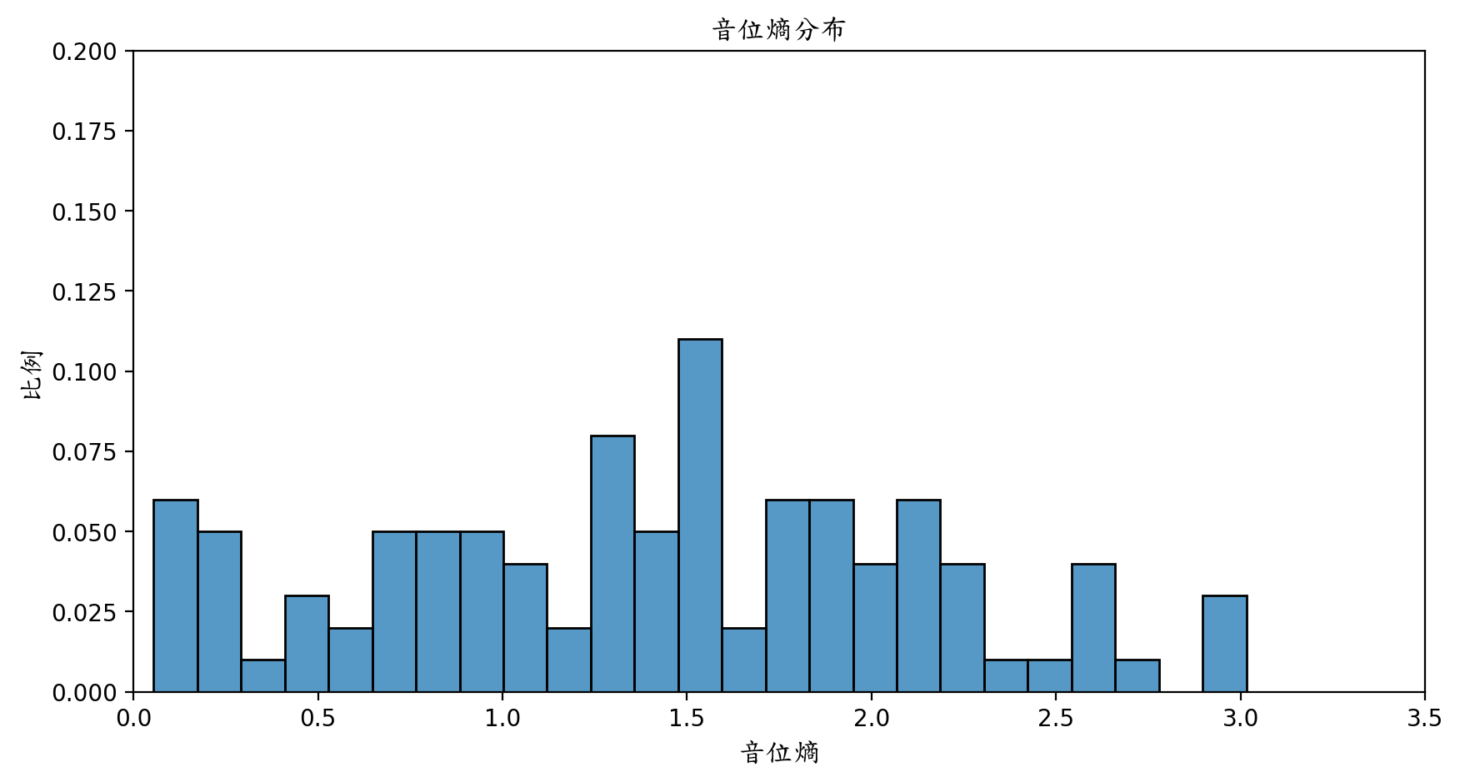
\includegraphics[width=\tempwidth]{figures/ch4figs/hub-u100-ap0000-phnent-hist.png}
                 \caption{離散單元}
                 \label{fig:hub-u100-ap0000-phnent-hist}
             \end{subfigure}
             \vfill
             \begin{subfigure}{\textwidth}
                 \centering
                 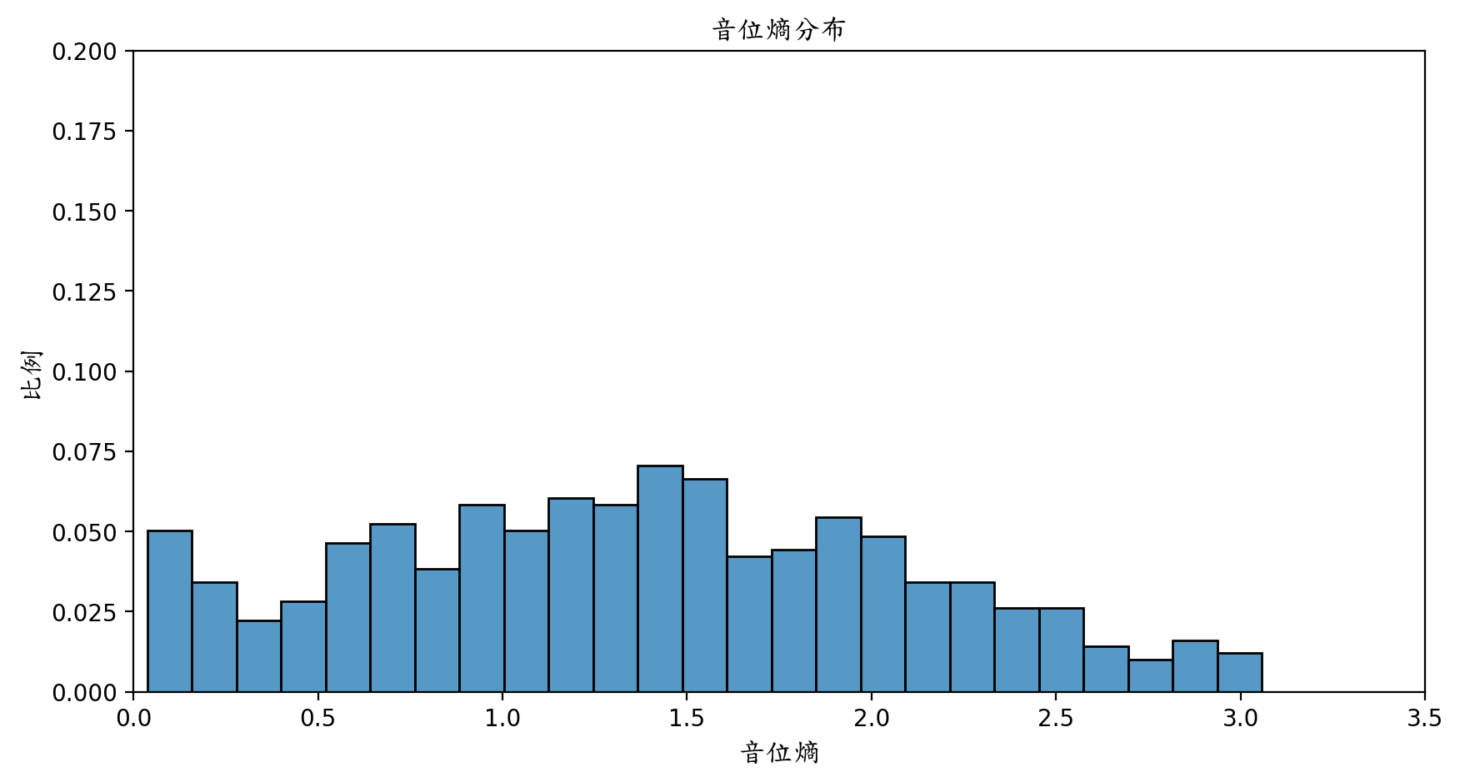
\includegraphics[width=\tempwidth]{figures/ch4figs/hub-u100-ap0500-phnent-hist.png}
                 \caption{500 種次詞單位}
                 \label{fig:hub-u100-ap0500-phnent-hist}
             \end{subfigure}
             \vfill
             \begin{subfigure}{\textwidth}
                 \centering
                 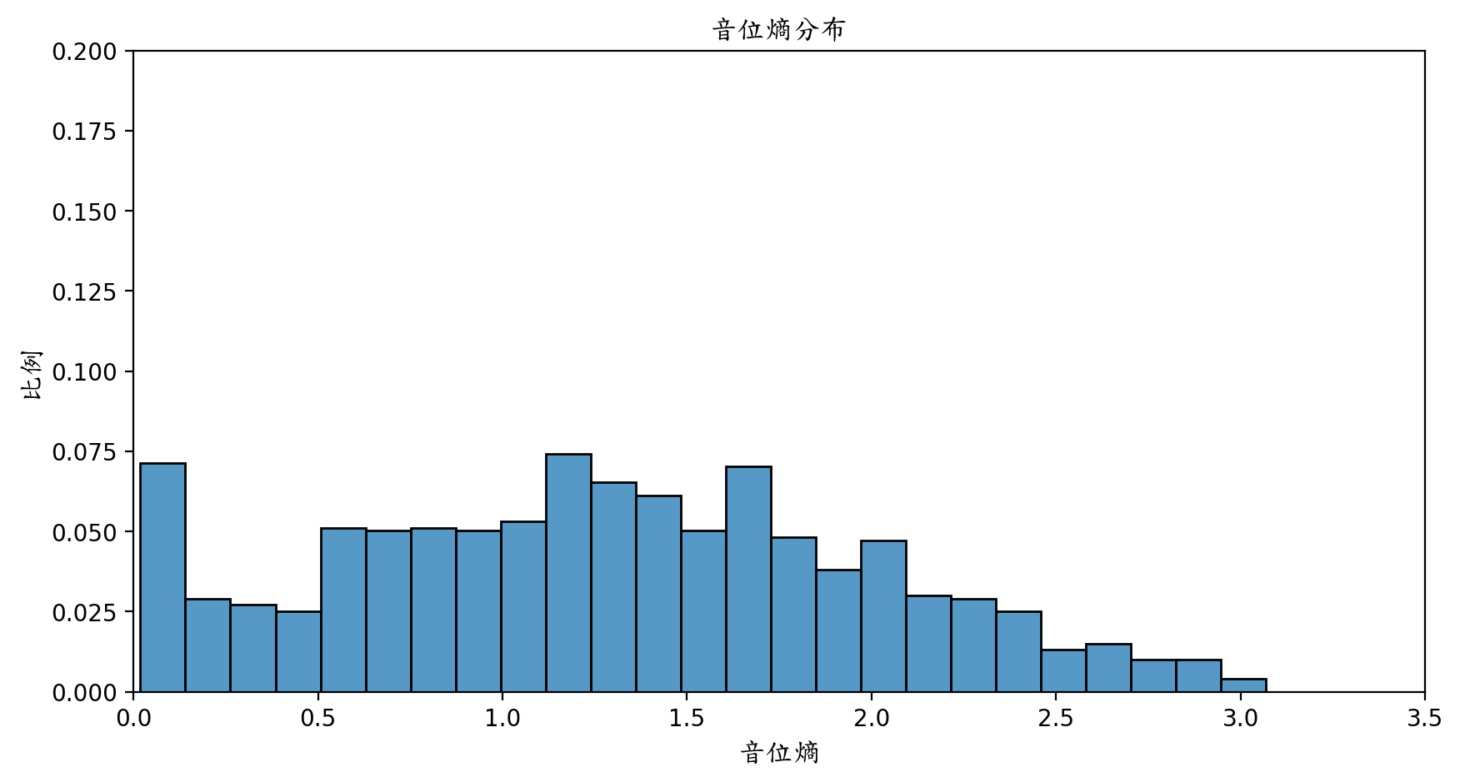
\includegraphics[width=\tempwidth]{figures/ch4figs/hub-u100-ap1000-phnent-hist.png}
                 \caption{1000 種次詞單位}
                 \label{fig:hub-u100-ap1000-phnent-hist}
             \end{subfigure}

             \caption{HuBERT 表徵在 K-平均演算法使用分群數 100 後,}
             比較不同次詞單位數量的音位條件熵 $H(y|z)$ 直方圖
             \label{fig:hub-u100-hist-comparisons}
        \end{figure}
    }
}


表 \ref{tab:hubert-phn-results-} 是 HuBERT 模型透過離散單元與不同次詞單位數量之聲學片段的純度與相互資訊數據。
首先,為了觀察聲學片段數量對於機率熱圖與純度數據的影響,圖 \ref{fig:hub-u050-comparisons} 與圖 \ref{fig:hub-u100-comparisons} 分別以
HuBERT 表徵、分群數為 50 和 100 的離散單元為基礎,比較原始離散單元、500 和 1000 種次詞單位三種設定下,不同聲學片段數量的條件機率熱圖。\jcm{它們分別是 HuBERT 模型配合分群數為 50 和 100 的離散單元模型,並將各自的離散單元使用單一詞演算法得到次詞單位數量為 500 和 1000 的聲學片段所得到的結果。}從中我們可以看出,當聲學片段數量上升時,熱圖可以觀察出許多更深的色塊,也就是有更多的聲學片段可以更集中的對應到特定音位。由此可見,有了更多樣的符記可以區別出更細節的發音差異,使整體的純度數值有所提升;然而,機率熱圖整體也變得更加破碎,因此歸類同樣音位的效果也相對變得較不明顯。

        為了確認各自聲學片段對應音位之集中狀況,我們可以考慮這些機率熱圖的條件音位熵 $H(y|z)$,以直方圖呈現來確認變化。透過觀察圖 \ref{fig:hub-u050-hist-comparisons} 與圖 \ref{fig:hub-u100-hist-comparisons} 的結果,可以確認相比第三章的離散單元,引入次詞單位確實能降低整體的條件音位熵,亦即新的符記各自能夠有更明確對應的音位,與我們從機率熱圖上所觀察到的趨勢符合。
        

        雖然改用聲學片段會使熱圖更加破碎而複雜,
% 難以觀察,
但
除純度與相互資訊的數值變化外,
觀察每個聲學片段對應之最高機率音位 $i^*(j)$ 以及它們的音位分類比例變化,
% 從符記代表性音位的比例變化,
也可以驗證「更多符記可以區別發音細節差異」這點。
再次觀察 HuBERT 在分群數 50 時的機率熱圖(圖 \ref{fig:hub-u050-comparisons}),圖 \ref{fig:hub-u050-comparisons} 中三章熱圖的藍色鉛直線
是
每個符記
在找出對應音位 $i^*(j)$ 後,按音位分類分區排序的結果。
因此,比較藍色鉛直線在橫軸上各區的比例變化,
可以知道
有多少比例的符記
能表示
特定類型的發音。
% 這些符記以多少的比例對應不同音位的發音特徵。
% \textcolor{red}{0000000000000000000000000000000000000000}
第三章結尾時提及過,在離散單元分群數為 50 時,由於符記數量較少,並沒有任何單元最能直接對應塞擦音音位。然而,當將這些離散單元以次詞單位進行重組後,不管在新符記種數為 500 或 1000 的機率熱圖上,都可以發現至少出現一個以上的符記得以對應到塞擦音。由此,我們驗證了引入次詞單位,對捕捉更細微的發音差異的確有所幫助。

\subsubsection{離散單元分群數對聲學片段表現的影響}

{
    {
        \begin{figure}
             \centering
             \begin{subfigure}{\textwidth}
                 \centering
                 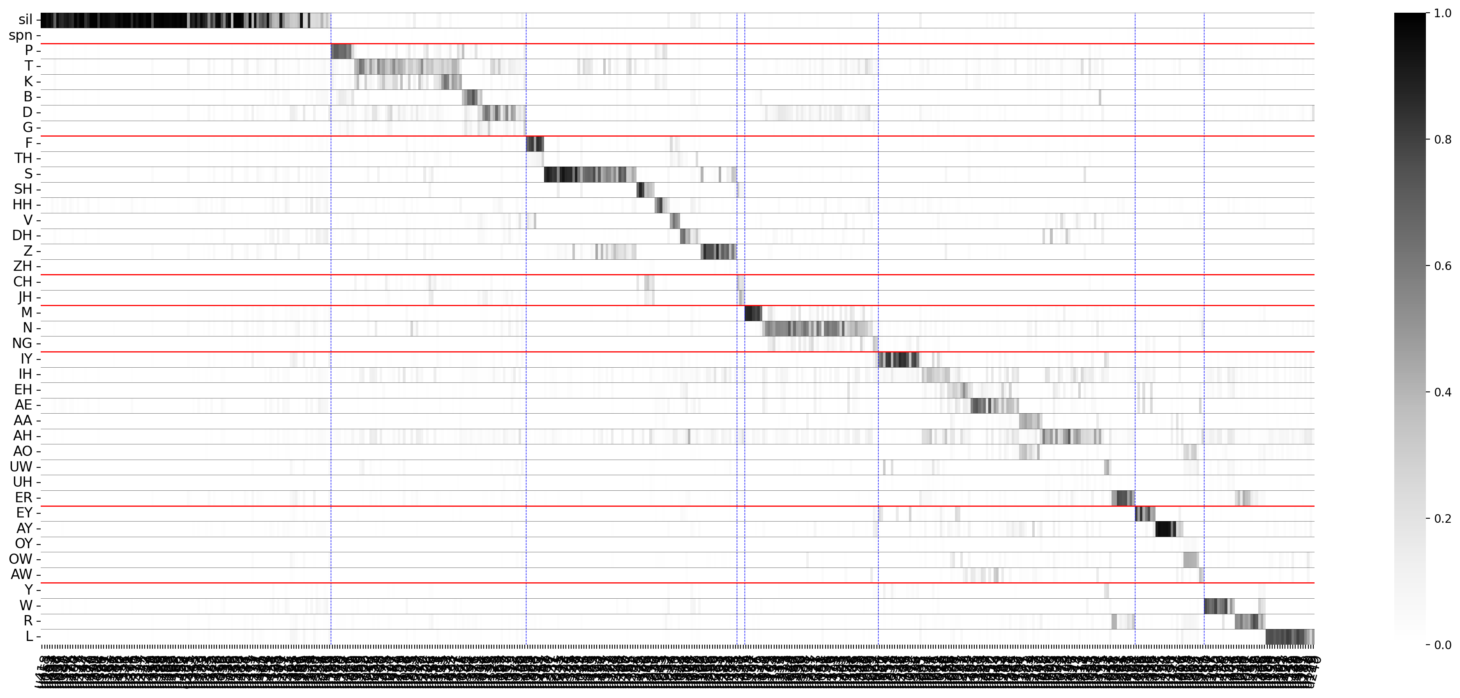
\includegraphics[width=1\linewidth]{figures/ch4figs/hub-u050-ap0500-givenunit-byphn.png}
                 \caption{分群數 50}
                 \label{fig:hub-u050-ap0500-givenunit-byphn--picked}
             \end{subfigure}
             \vfill
             \begin{subfigure}{\textwidth}
                 \centering
                 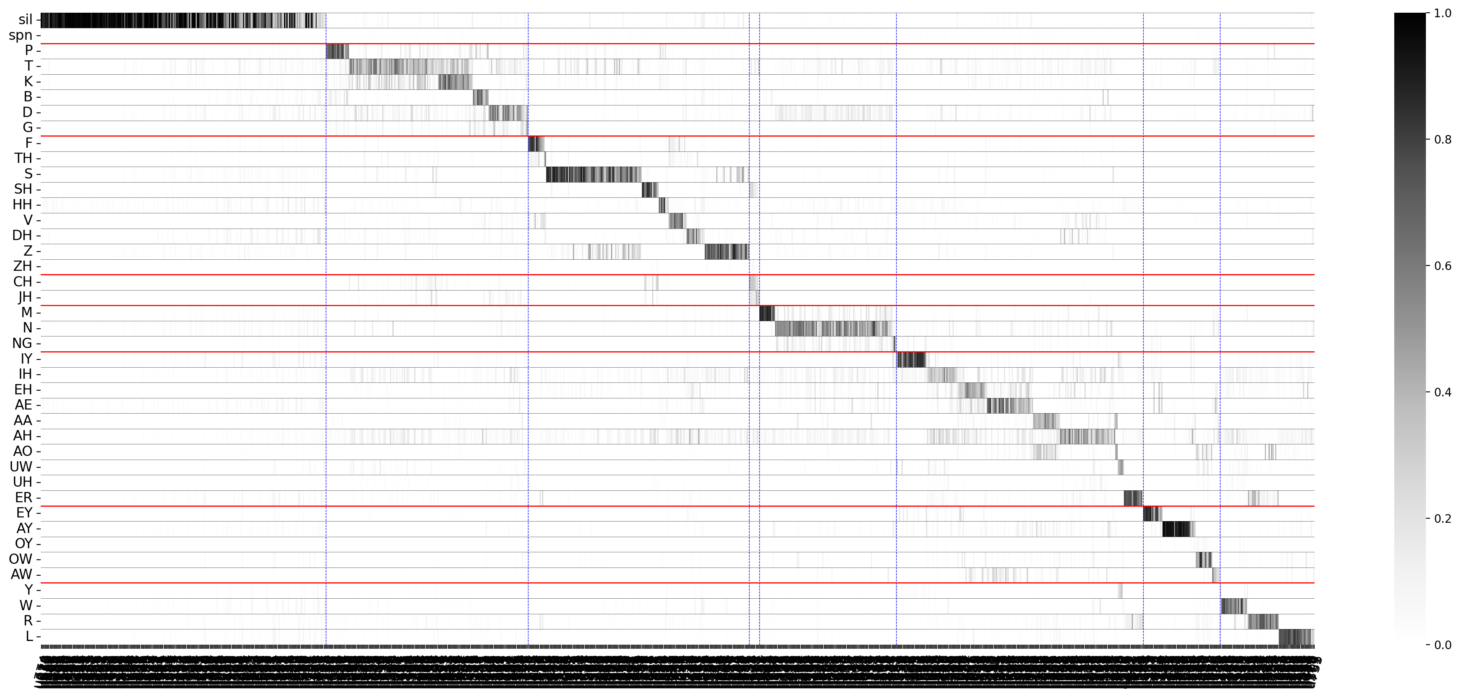
\includegraphics[width=1\linewidth]{figures/ch4figs/hub-u050-ap1000-givenunit-byphn.png}
                 \caption{分群數 100}
                 \label{fig:hub-u100-ap0500-givenunit-byphn--picked}
             \end{subfigure}
             \caption{比較同樣 500 種次詞單位的聲學片段模型,著重比較 HuBERT 表徵}
             在 K-平均演算法使用分群數 50 與 100 的條件機率熱圖 $p_{y|z}(i|j)$ 差異
             \label{fig:check-ap0500}
        \end{figure}
    }
}

  然而,儘管引入次詞單位一定程度上能幫助區別語音訊號中的細微發音差異,
% 若要更直接的改善對這件事進行改善,
在語音表徵進行離散化時,
K-平均演算法的分群數仍是決定
這些符記捕捉語音資訊
更關鍵的決定因素。
圖 \ref{fig:check-ap0500} 比較了同樣是 500 種次詞單位,K-平均演算法的離散表徵分群數選擇 50 和 100 的機率熱圖差異,不難發現分群數為 100 的機率熱圖能更加平均的對應到不同音位。然而,即便與音位的對應效果\jcm{對音位標註的歸類效果}最大取決於 K-平均的分群數,但分群演算法本身
相當消耗計算資源。因此
當遇到運算資源限制,致使 K-平均演算法的分群數難以設置得很大時,次詞單位的引入仍舊能提升整體表現。
        \jcm{藉由比較幾章機率熱圖的差異,我們可以確認這件事。 \jcm{補寫一下}}

        \jcm{
        
        我們這邊可以比較一下 50、100、50+100、50+500、100+500 的熱圖。從這邊可以驗證前面所說的:在基底分群數確定的情形之下,的確一開始分群數開得比較大,整體對語音規律的捕捉效果就會比較好,但藉由分群方法的引入,至少 50 分群數可以藉由符記數提升的機會,來重新編碼語音中的結構,也就是雖然不如 K-平均演算法那樣因為直接做用於語音表徵空間,那麼好區分出發音的差異,但藉由分詞演算法,仍然可以從捕捉語音中明顯重複的序列資訊\textcolor{red}{[這時候是不是要擺一下長度 & 常見 pattern 統計數據確認了?] } ,獲取語音序列中跟發音有關的特徵,進而模擬類似人類理解音位的過程。
        
        }
}

    {
        \newcommand{\tempwidth}[0]{0.8\linewidth}
        \begin{figure}
             \centering
             \begin{subfigure}{\textwidth}
                 \centering
                 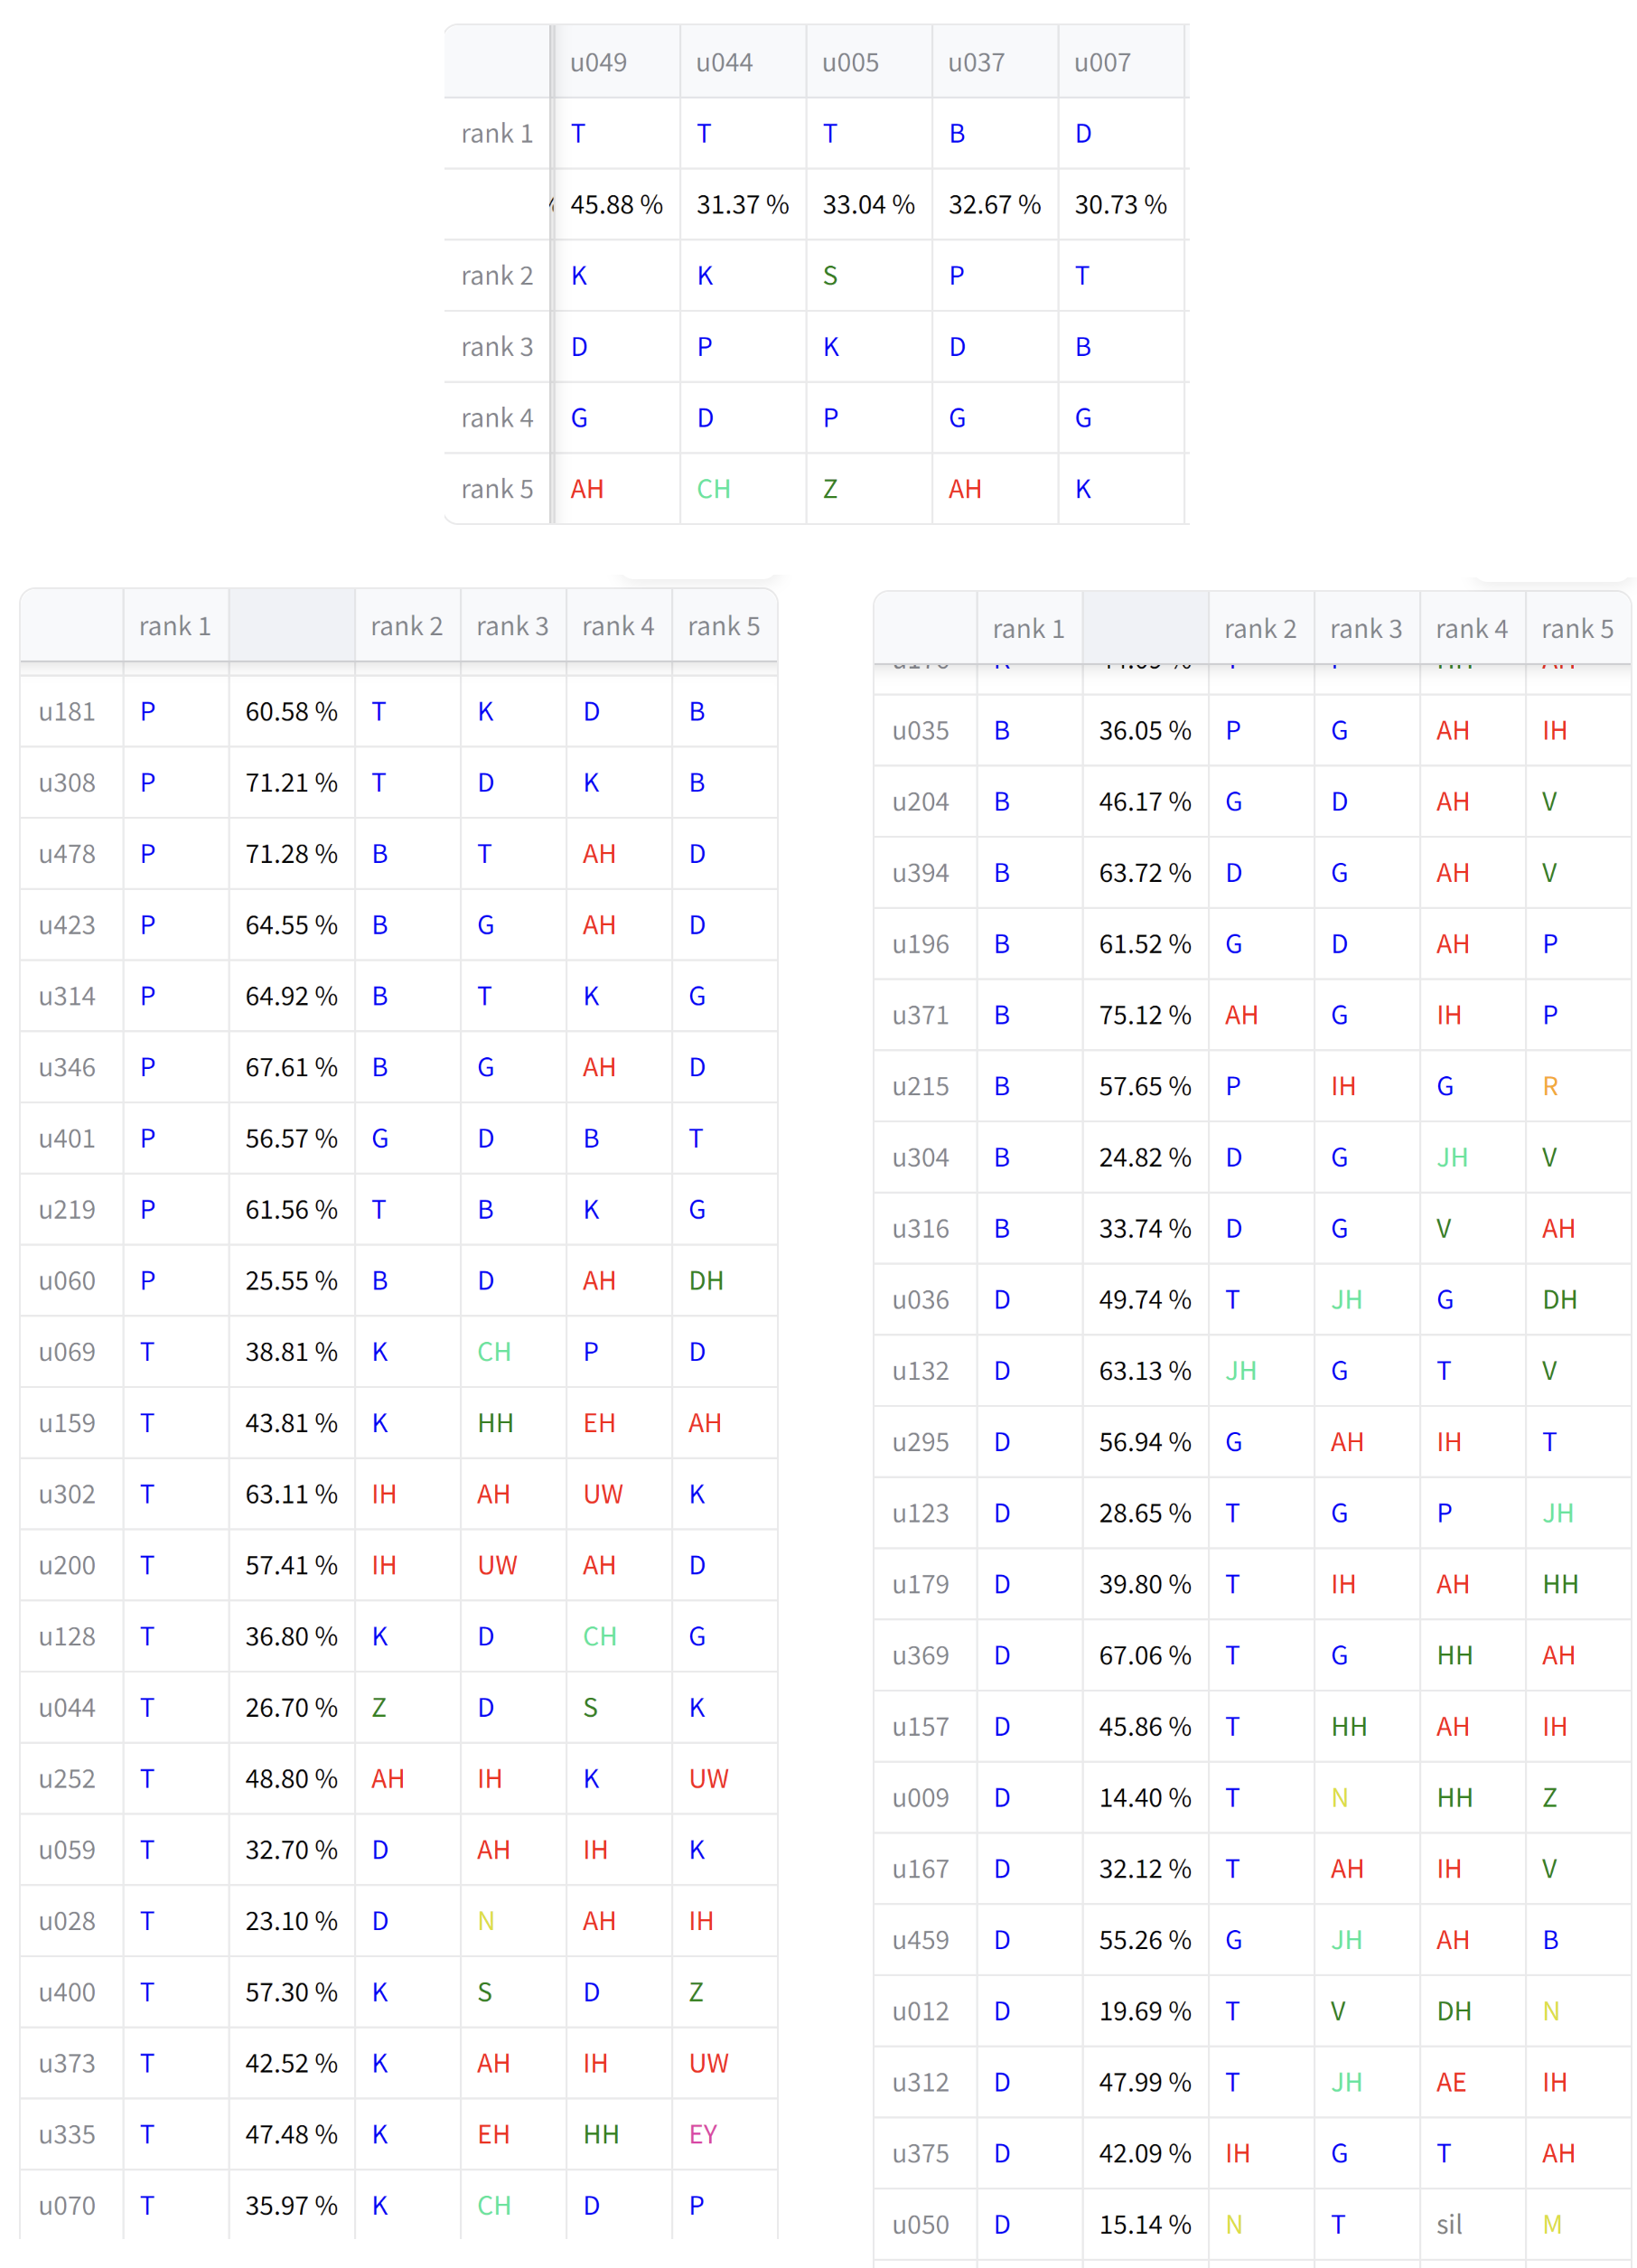
\includegraphics[width=\tempwidth]{figures/ch4figs/plo_phn.png}
                 \caption{塞音}
                 \label{fig:hub-u050-ap0500-ploobs}
             \end{subfigure}
             % \vfill
             % \begin{subfigure}{\textwidth}
             %     \centering
             %     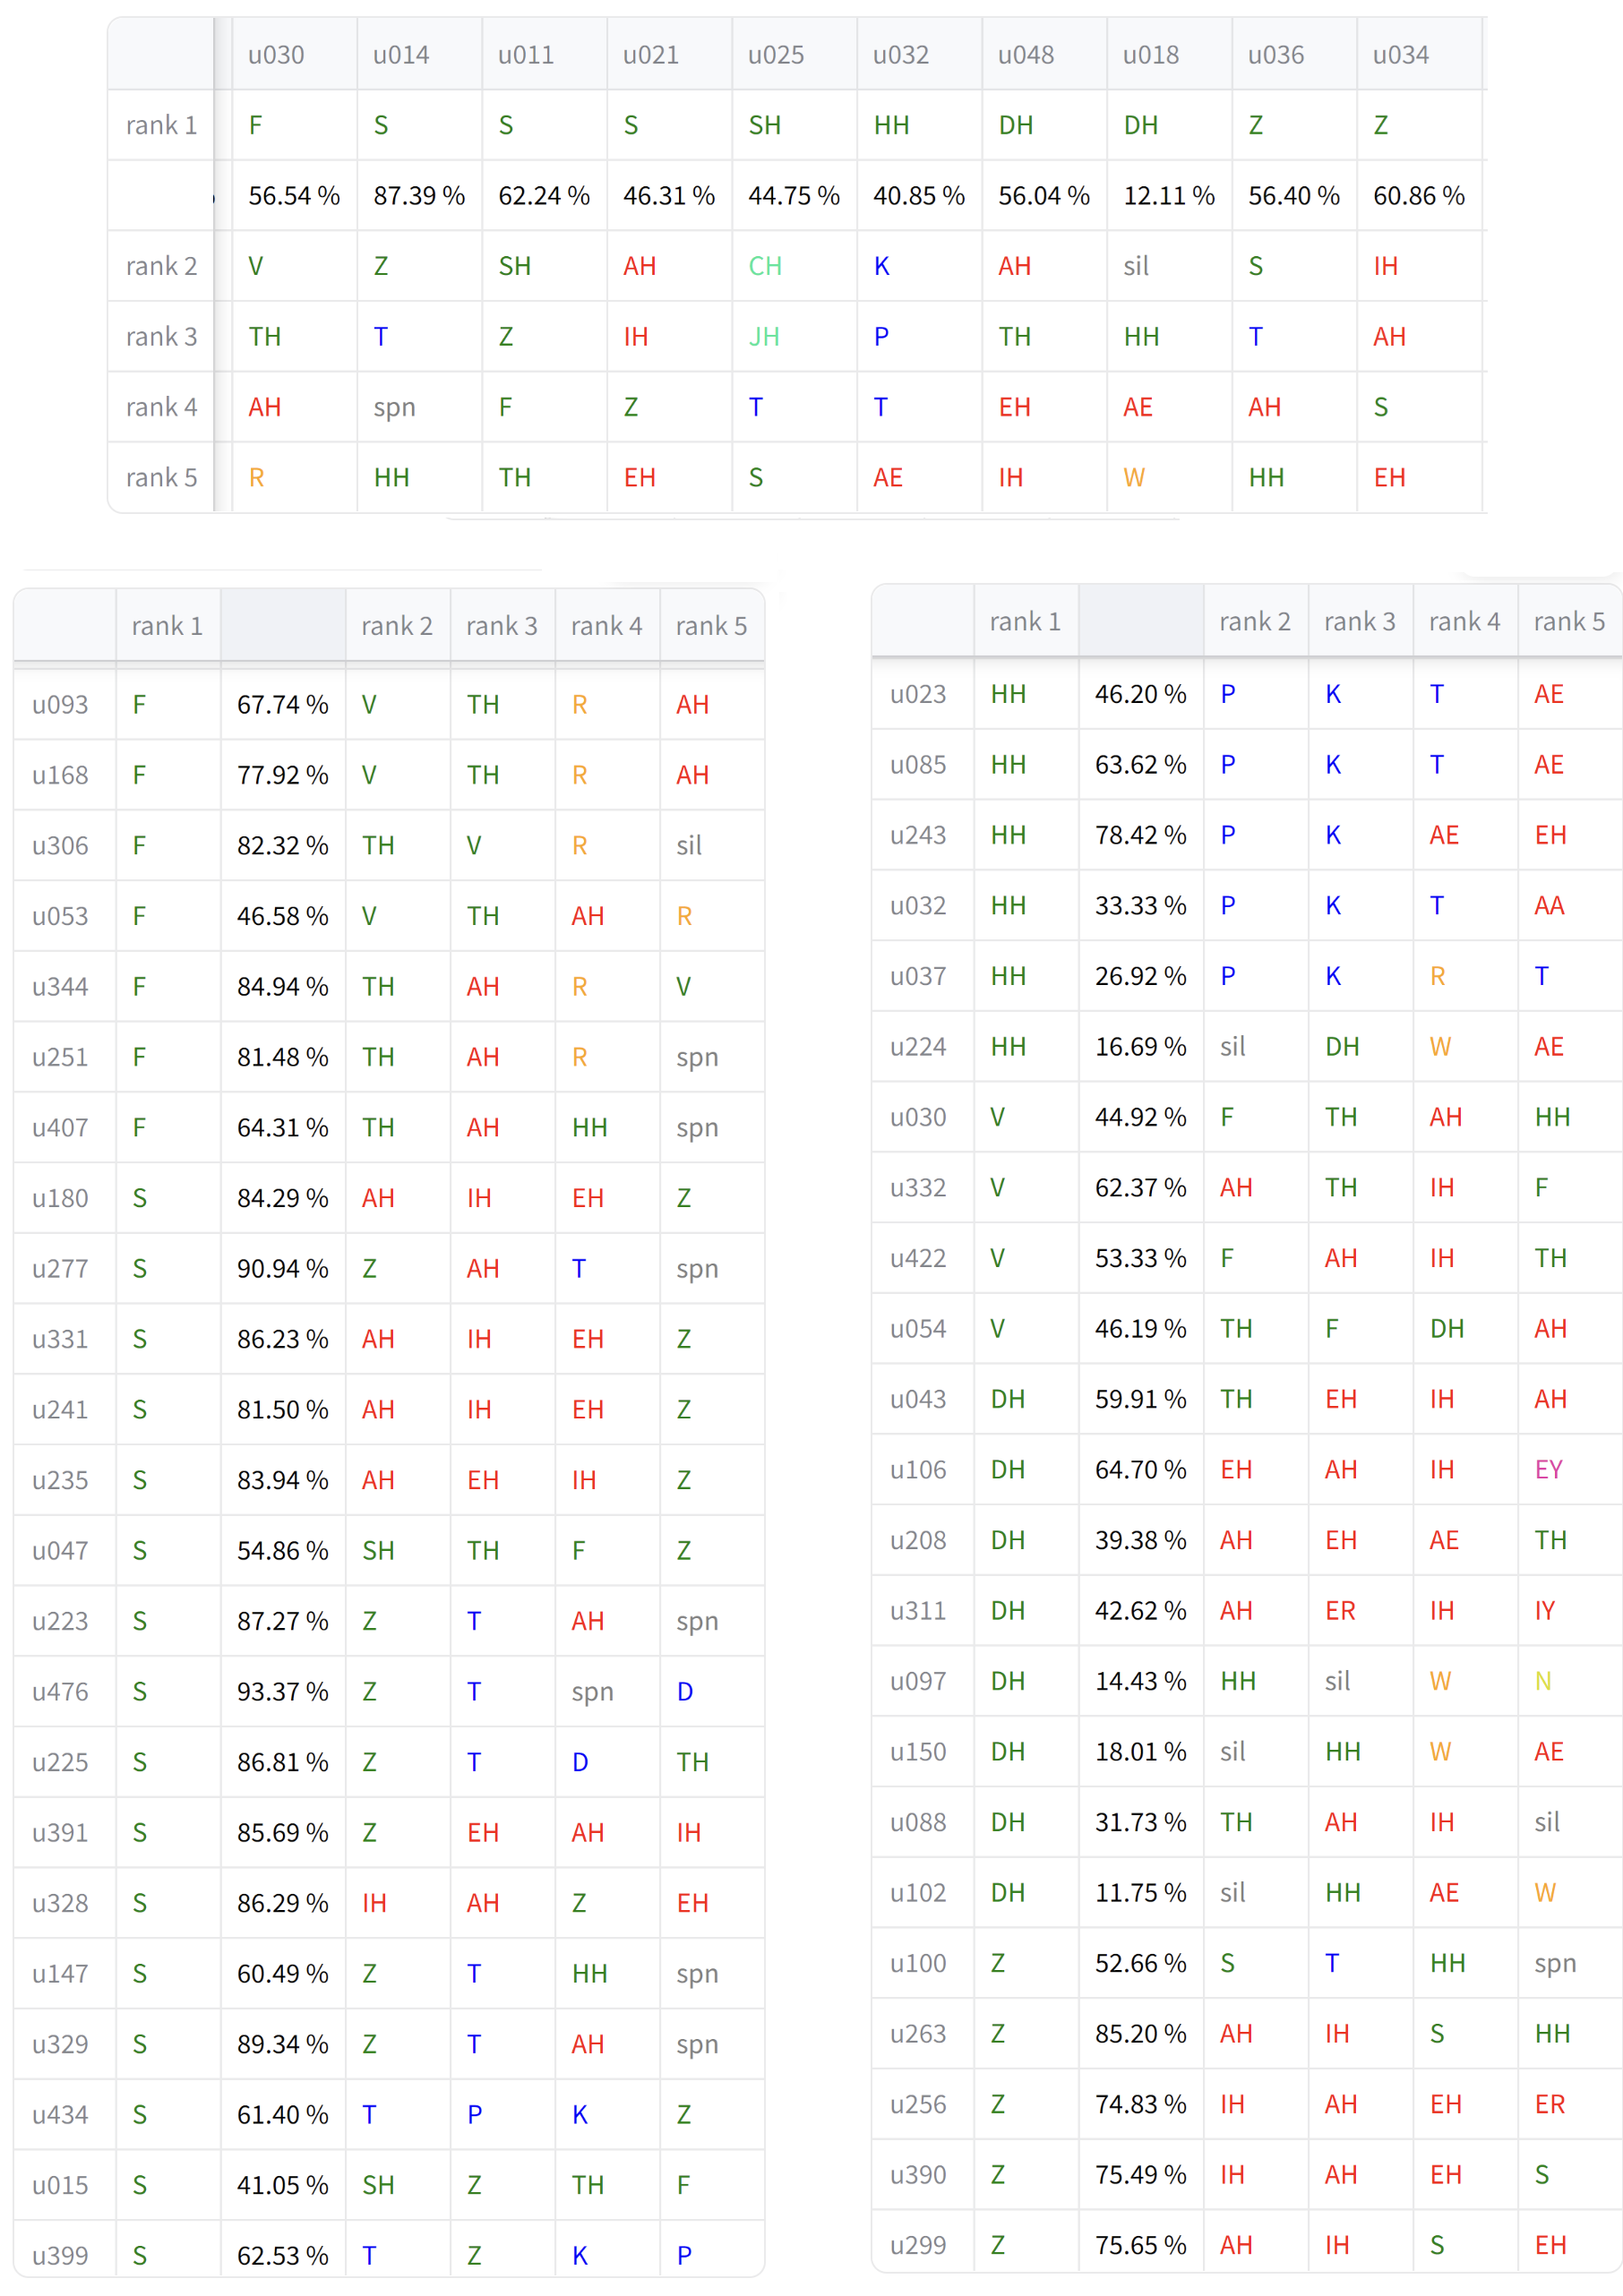
\includegraphics[width=\tempwidth]{figures/ch4figs/fri_phn.png}
             %     \caption{擦音}
             %     \label{fig:hub-u050-ap0500-friobs}
             % \end{subfigure}
             % \vfill
             % \begin{subfigure}{\textwidth}
             %     \centering
             %     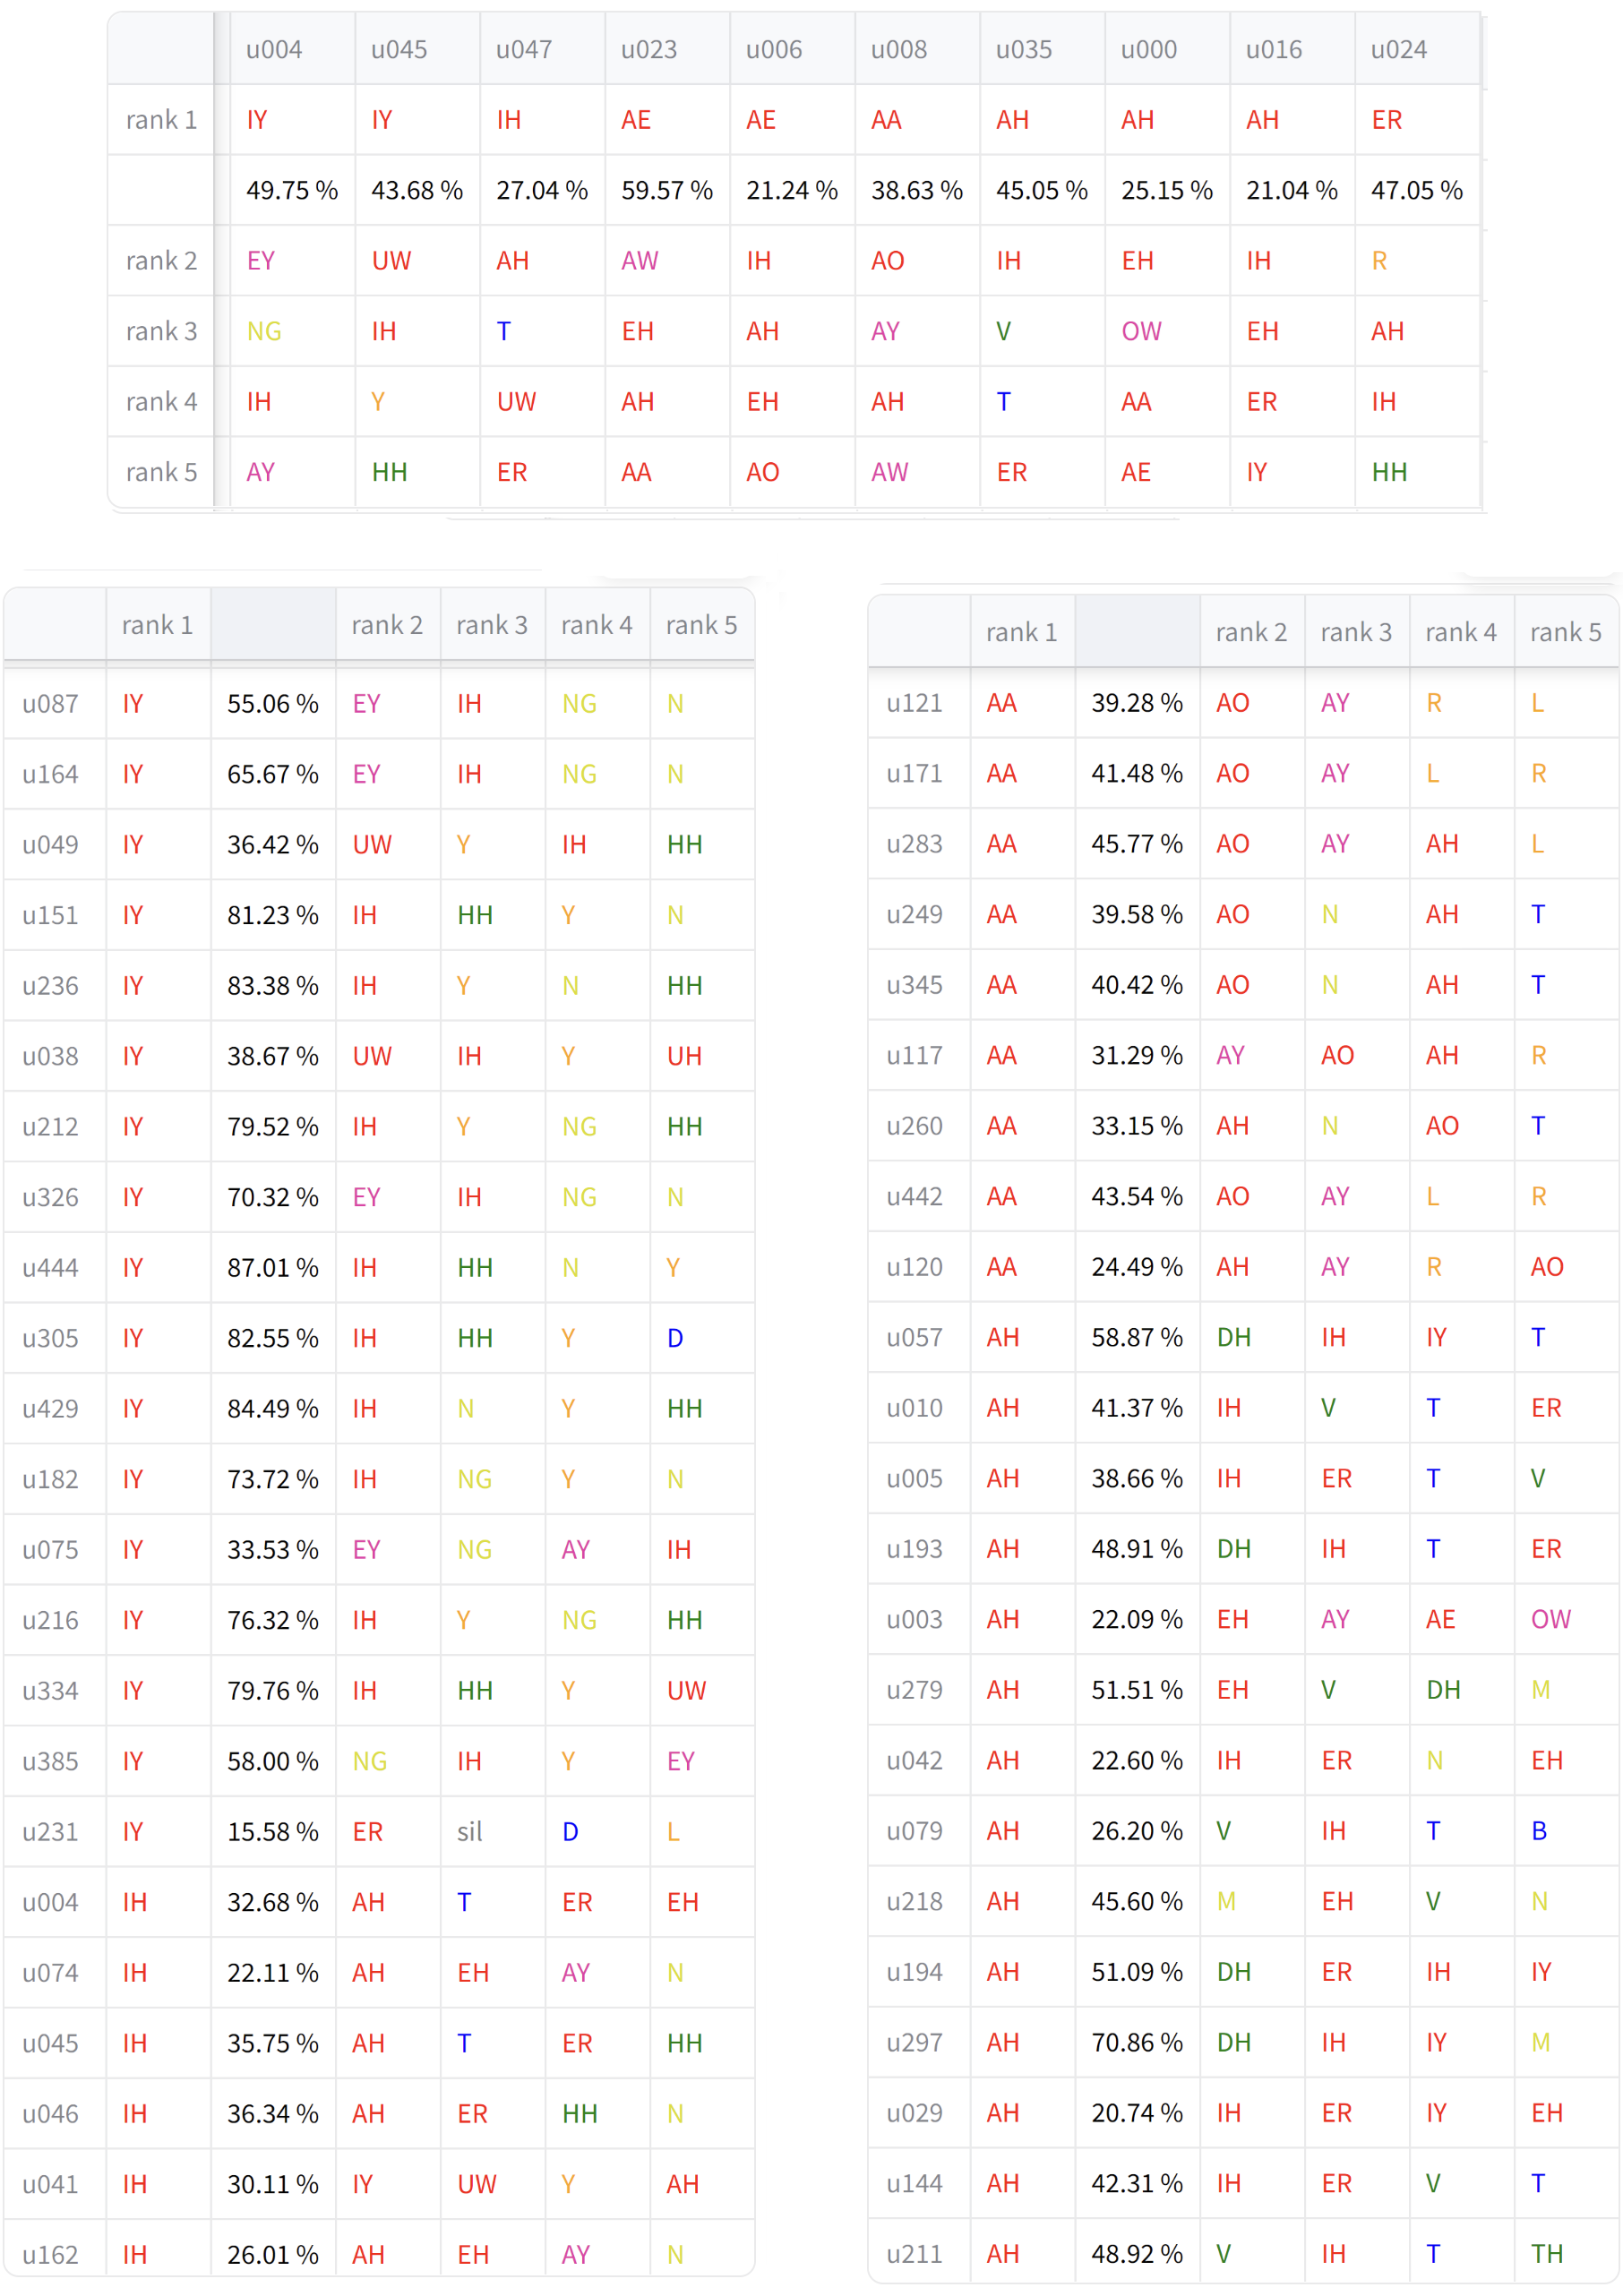
\includegraphics[width=\tempwidth]{figures/ch4figs/vow_phn.png}
             %     \caption{單元音}
             %     \label{fig:hub-u050-ap0500-vowobs}
             % \end{subfigure}

             \caption{HuBERT 表徵、K-平均演算法分群數 50,比較單一離散單元與}
             使用 500 種次詞單位,依據不同音位分類比較符記各自對應的前五高音位 \\
             上半部為離散單元,下半部為聲學片段。 \\
             圖中的百分比為最高機率音位的條件機率 $p_{y|z}(i^*(j)|j)$
                         \label{fig:hub-u050-phnobserver}
        \end{figure}
    }

        {
        \newcommand{\tempwidth}[0]{0.8\linewidth}
        \begin{figure}
        \ContinuedFloat
             \centering
             % \begin{subfigure}{\textwidth}
             %     \centering
             %     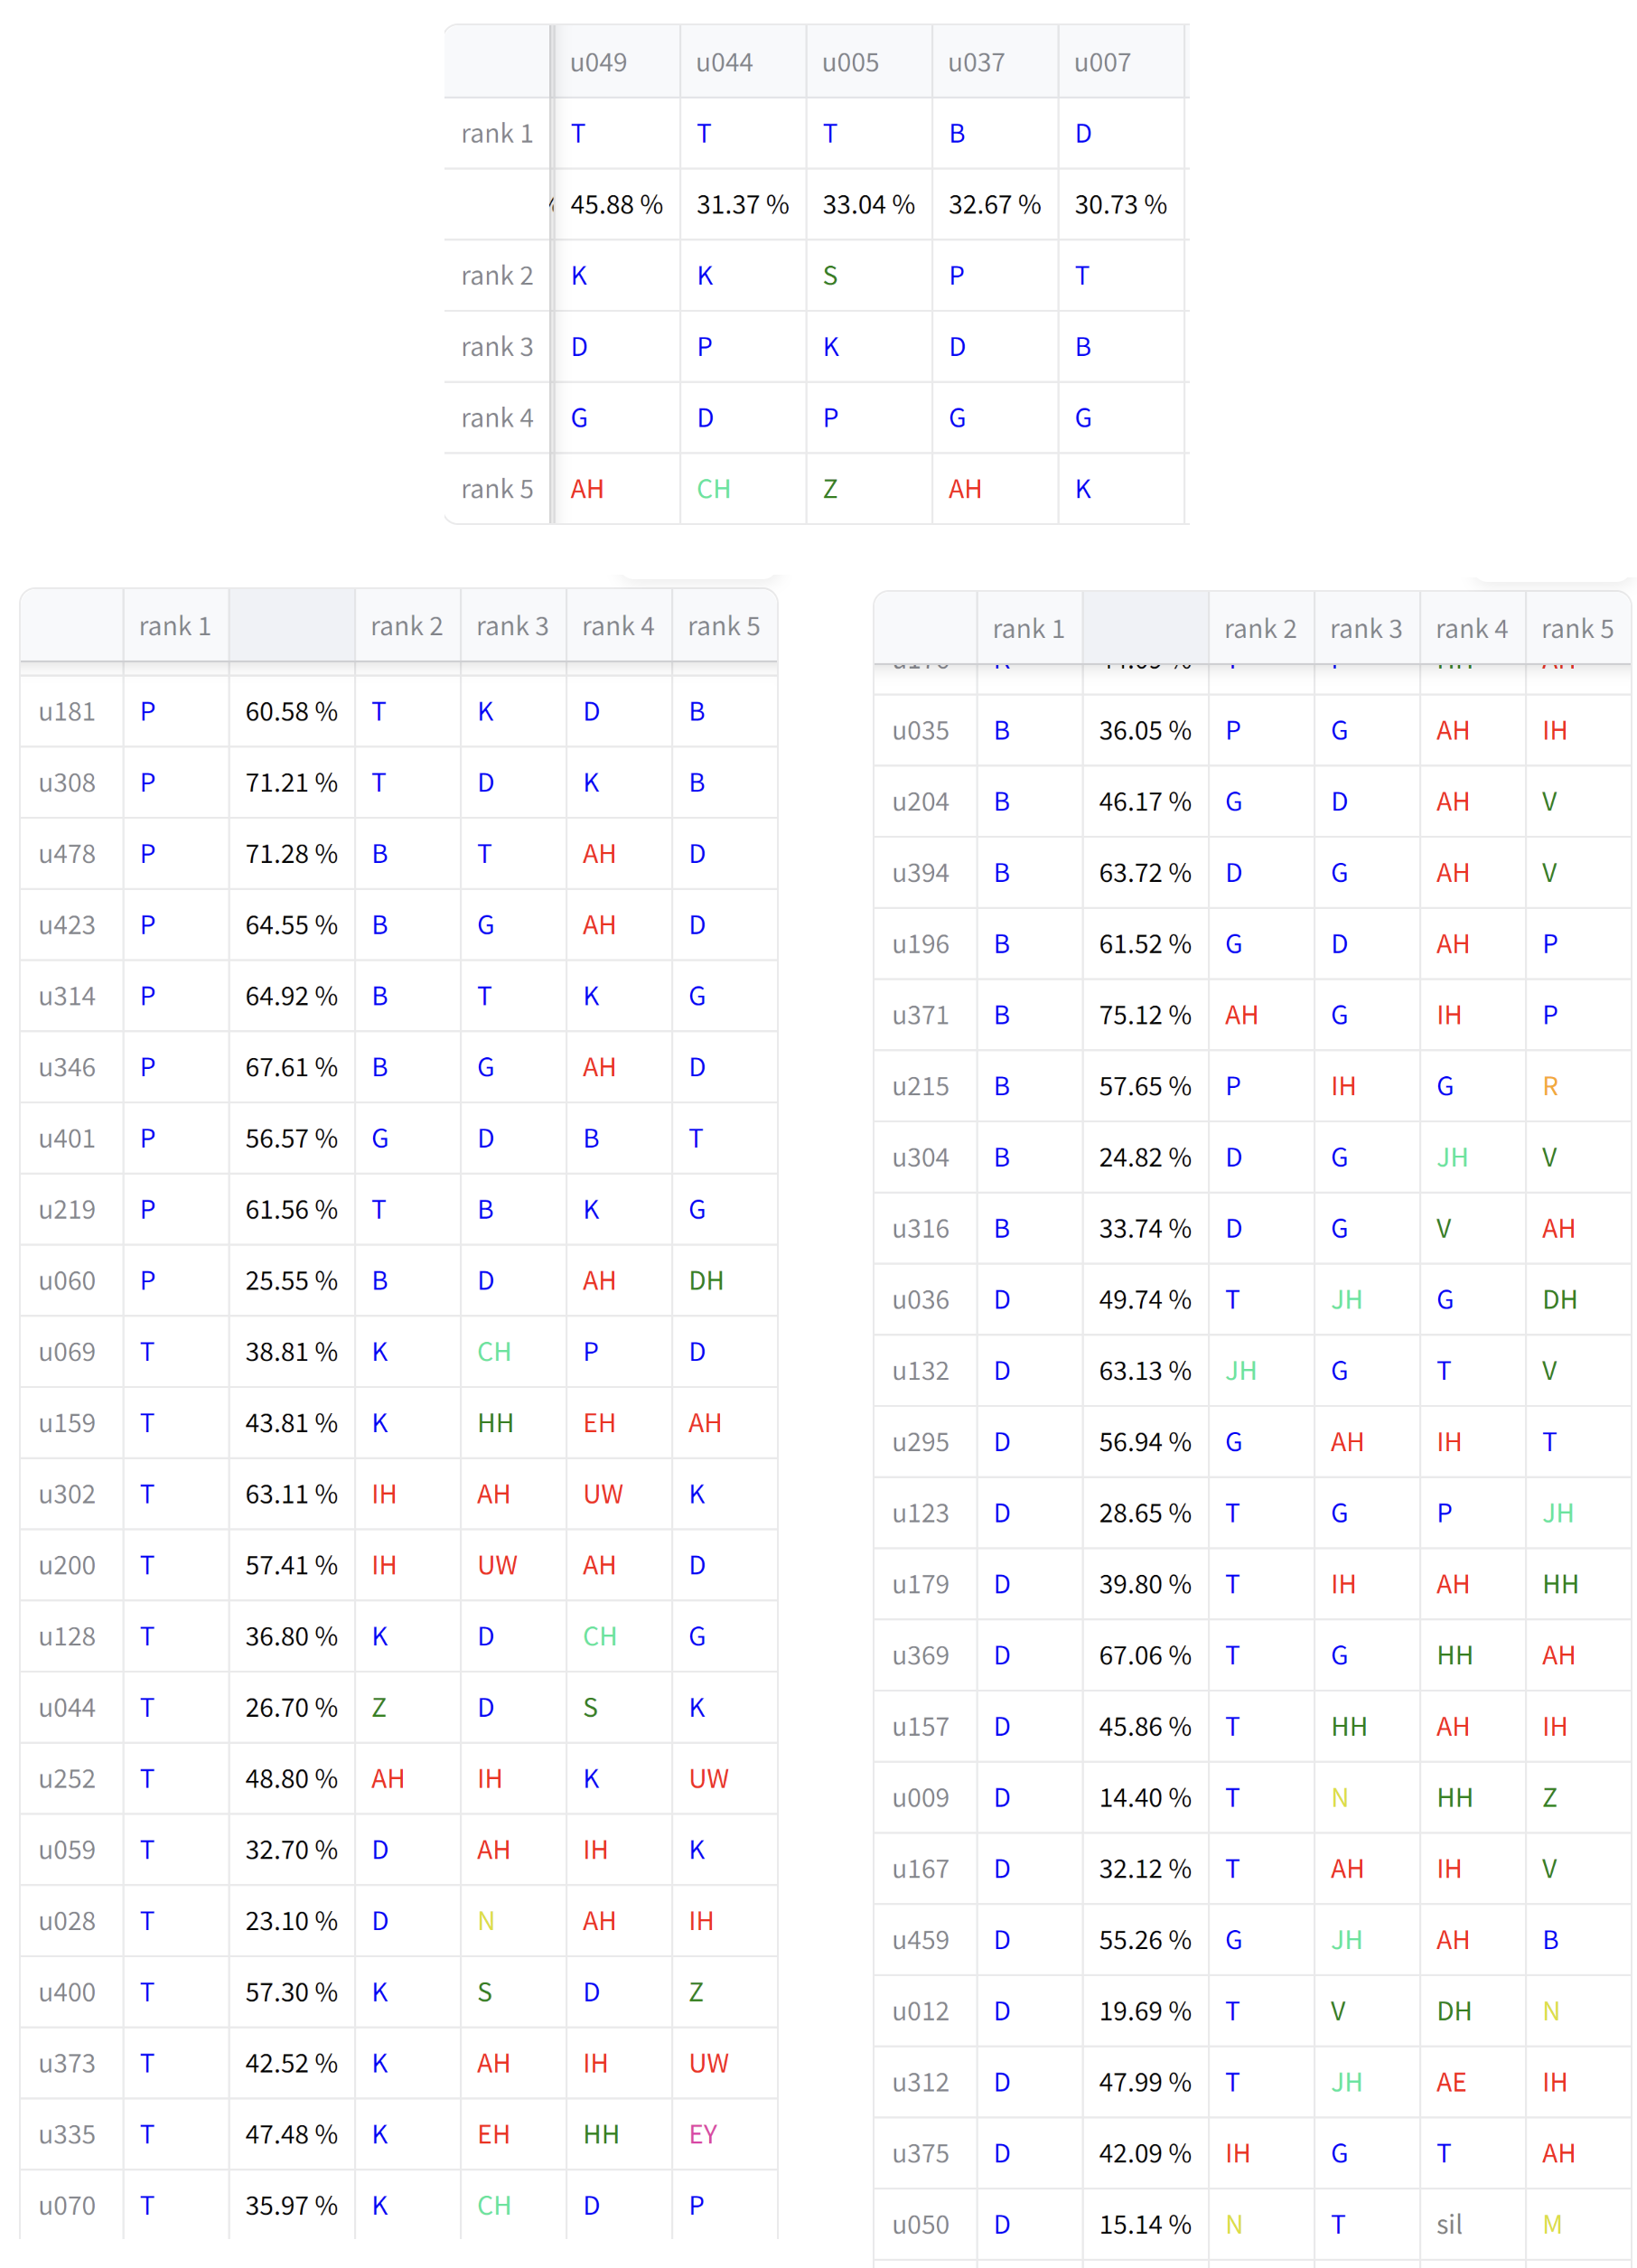
\includegraphics[width=\tempwidth]{figures/ch4figs/plo_phn.png}
             %     \caption{塞音}
             %     \label{fig:hub-u050-ap0500-ploobs}
             % \end{subfigure}
             % \vfill
             \begin{subfigure}{\textwidth}
                 \centering
                 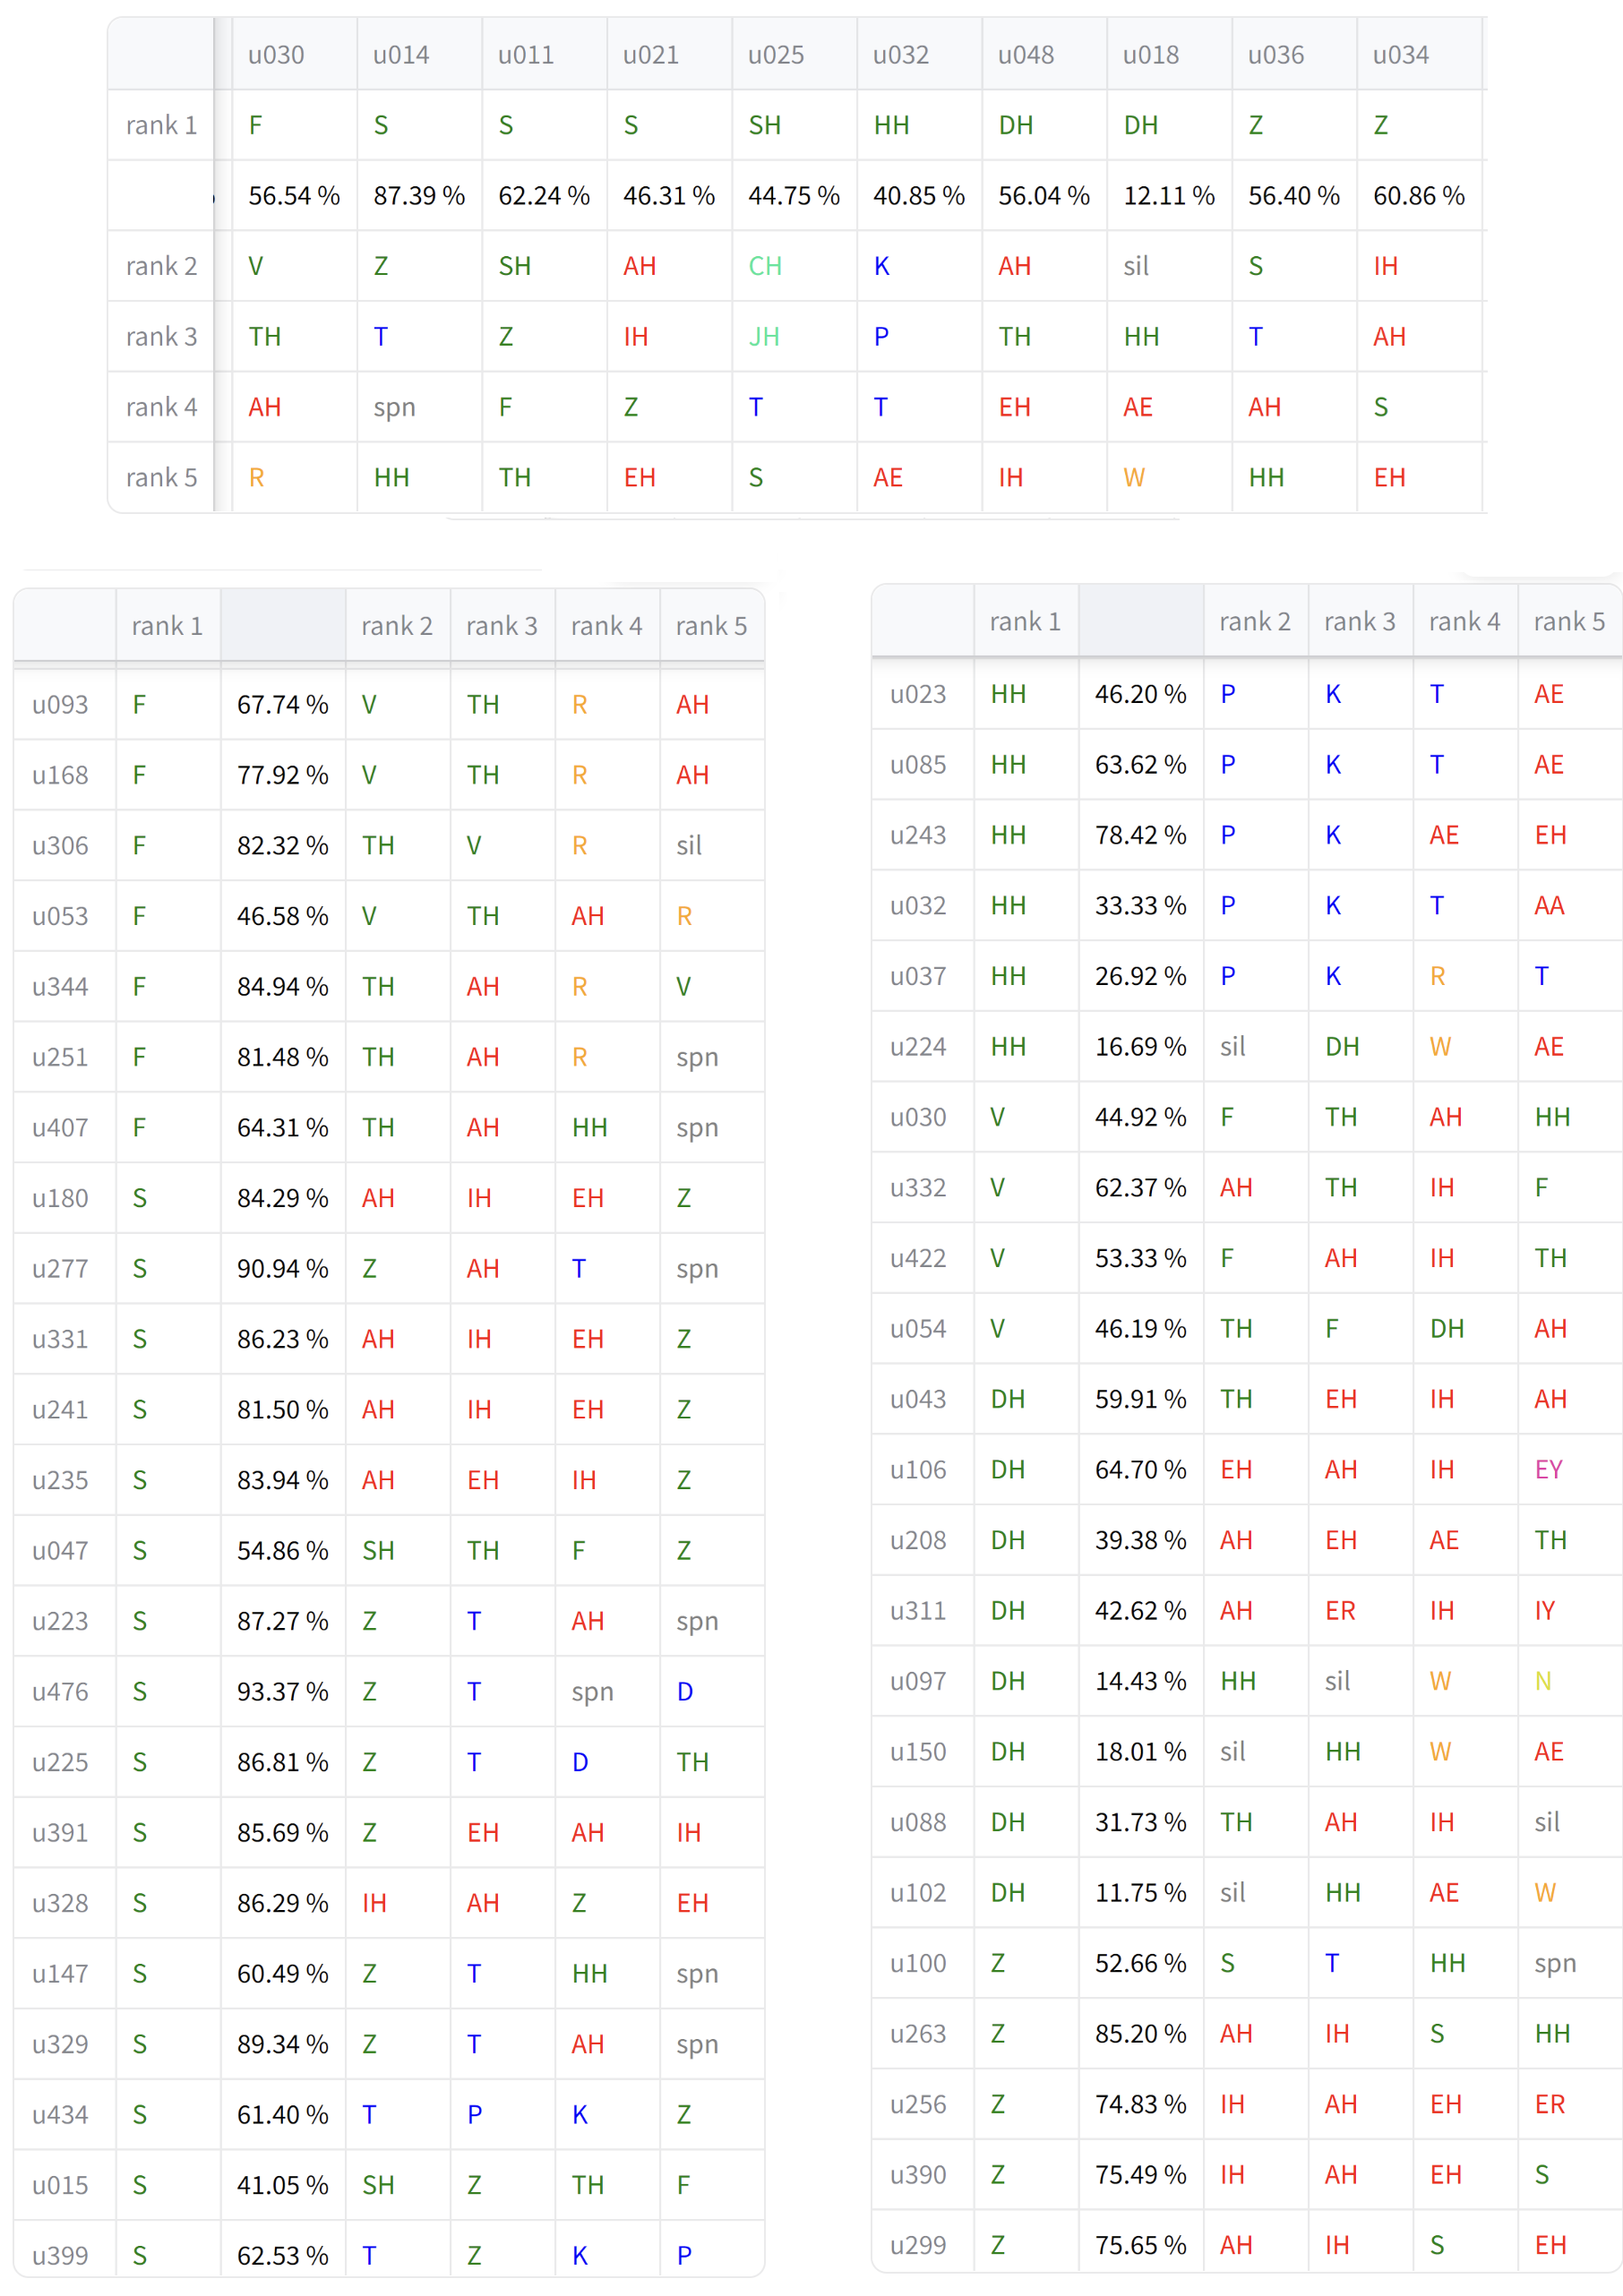
\includegraphics[width=\tempwidth]{figures/ch4figs/fri_phn.png}
                 \caption{擦音}
                 \label{fig:hub-u050-ap0500-friobs}
             \end{subfigure}
             % \vfill
             % \begin{subfigure}{\textwidth}
             %     \centering
             %     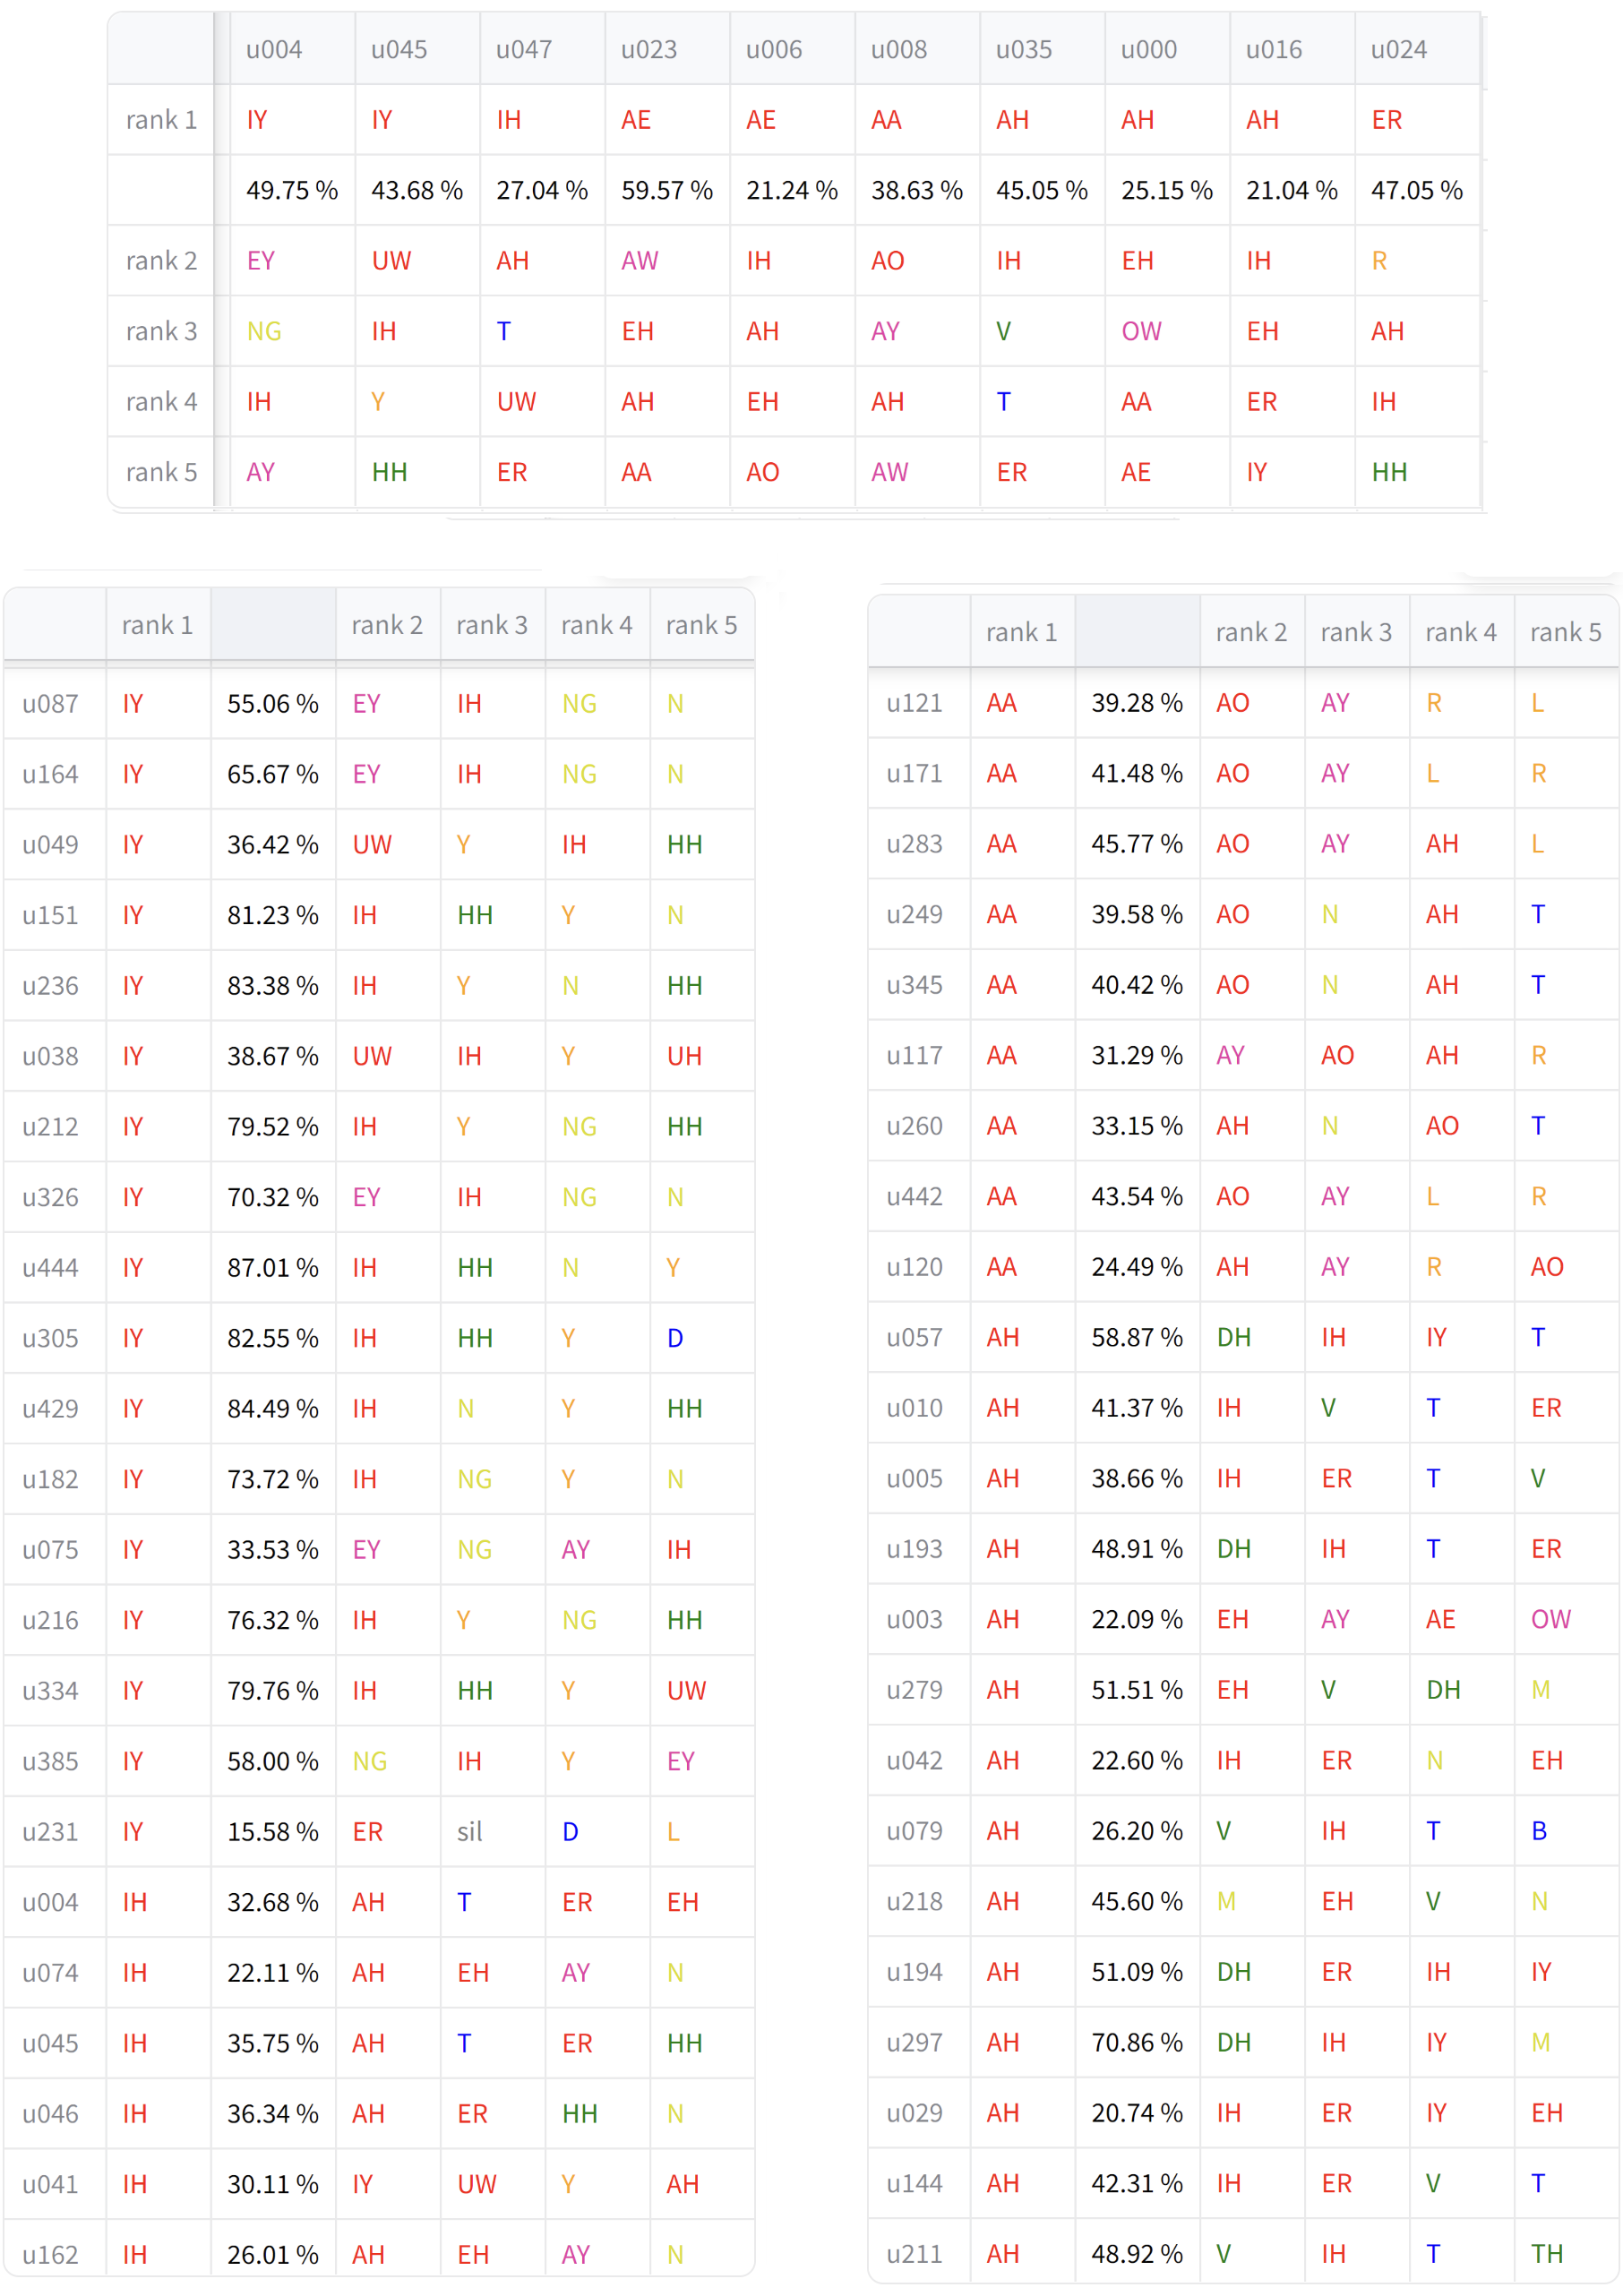
\includegraphics[width=\tempwidth]{figures/ch4figs/vow_phn.png}
             %     \caption{單元音}
             %     \label{fig:hub-u050-ap0500-vowobs}
             % \end{subfigure}

             % \caption{HuBERT 表徵、K-平均演算法分群數 50,比較單一離散單元與使用 500 種次詞單位,}
             % 依據不同音位分類比較符記各自對應的前五高音位
             % (上半部為離散單元,下半部為聲學片段。圖中的百分比為最高機率音位的條件機率 $p_{y|z}(i^*(j)|j)$)
                         \label{fig:hub-u050-phnobserver--2}
        \end{figure}
    }

        {
        \newcommand{\tempwidth}[0]{0.8\linewidth}
        \begin{figure}
        \ContinuedFloat
        
             \centering
             % \begin{subfigure}{\textwidth}
             %     \centering
             %     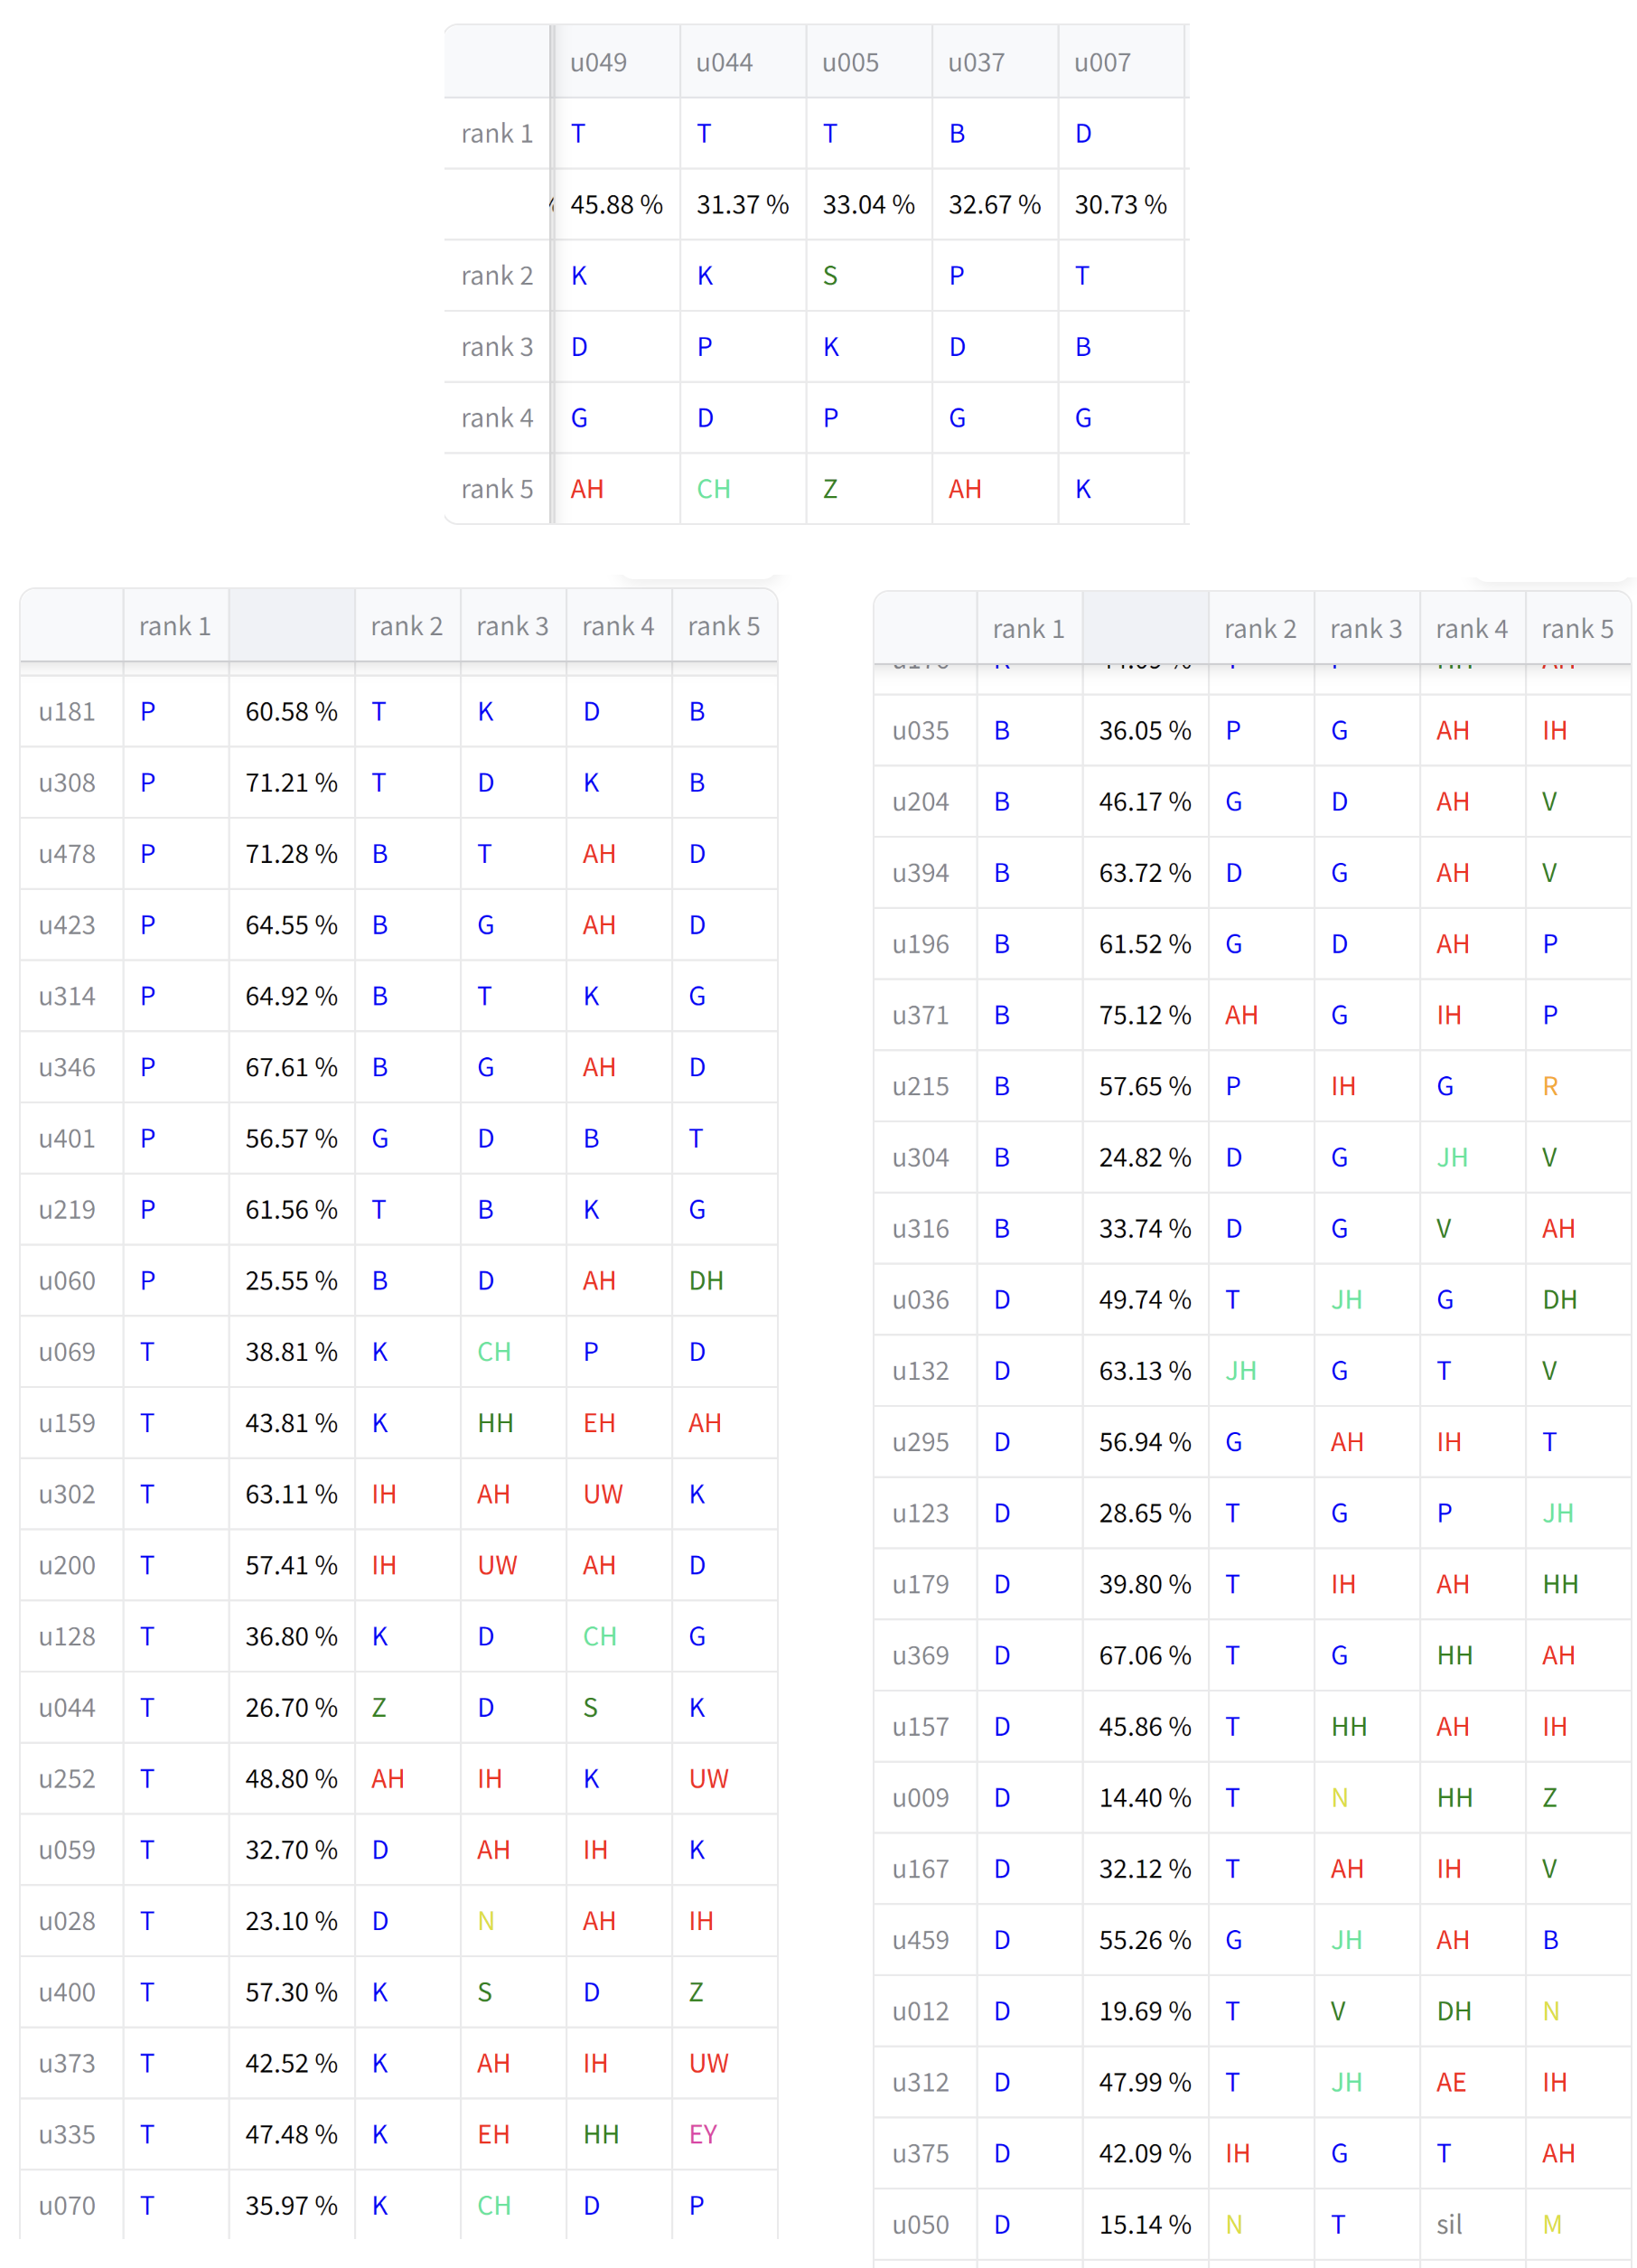
\includegraphics[width=\tempwidth]{figures/ch4figs/plo_phn.png}
             %     \caption{塞音}
             %     \label{fig:hub-u050-ap0500-ploobs}
             % \end{subfigure}
             % \vfill
             % \begin{subfigure}{\textwidth}
             %     \centering
             %     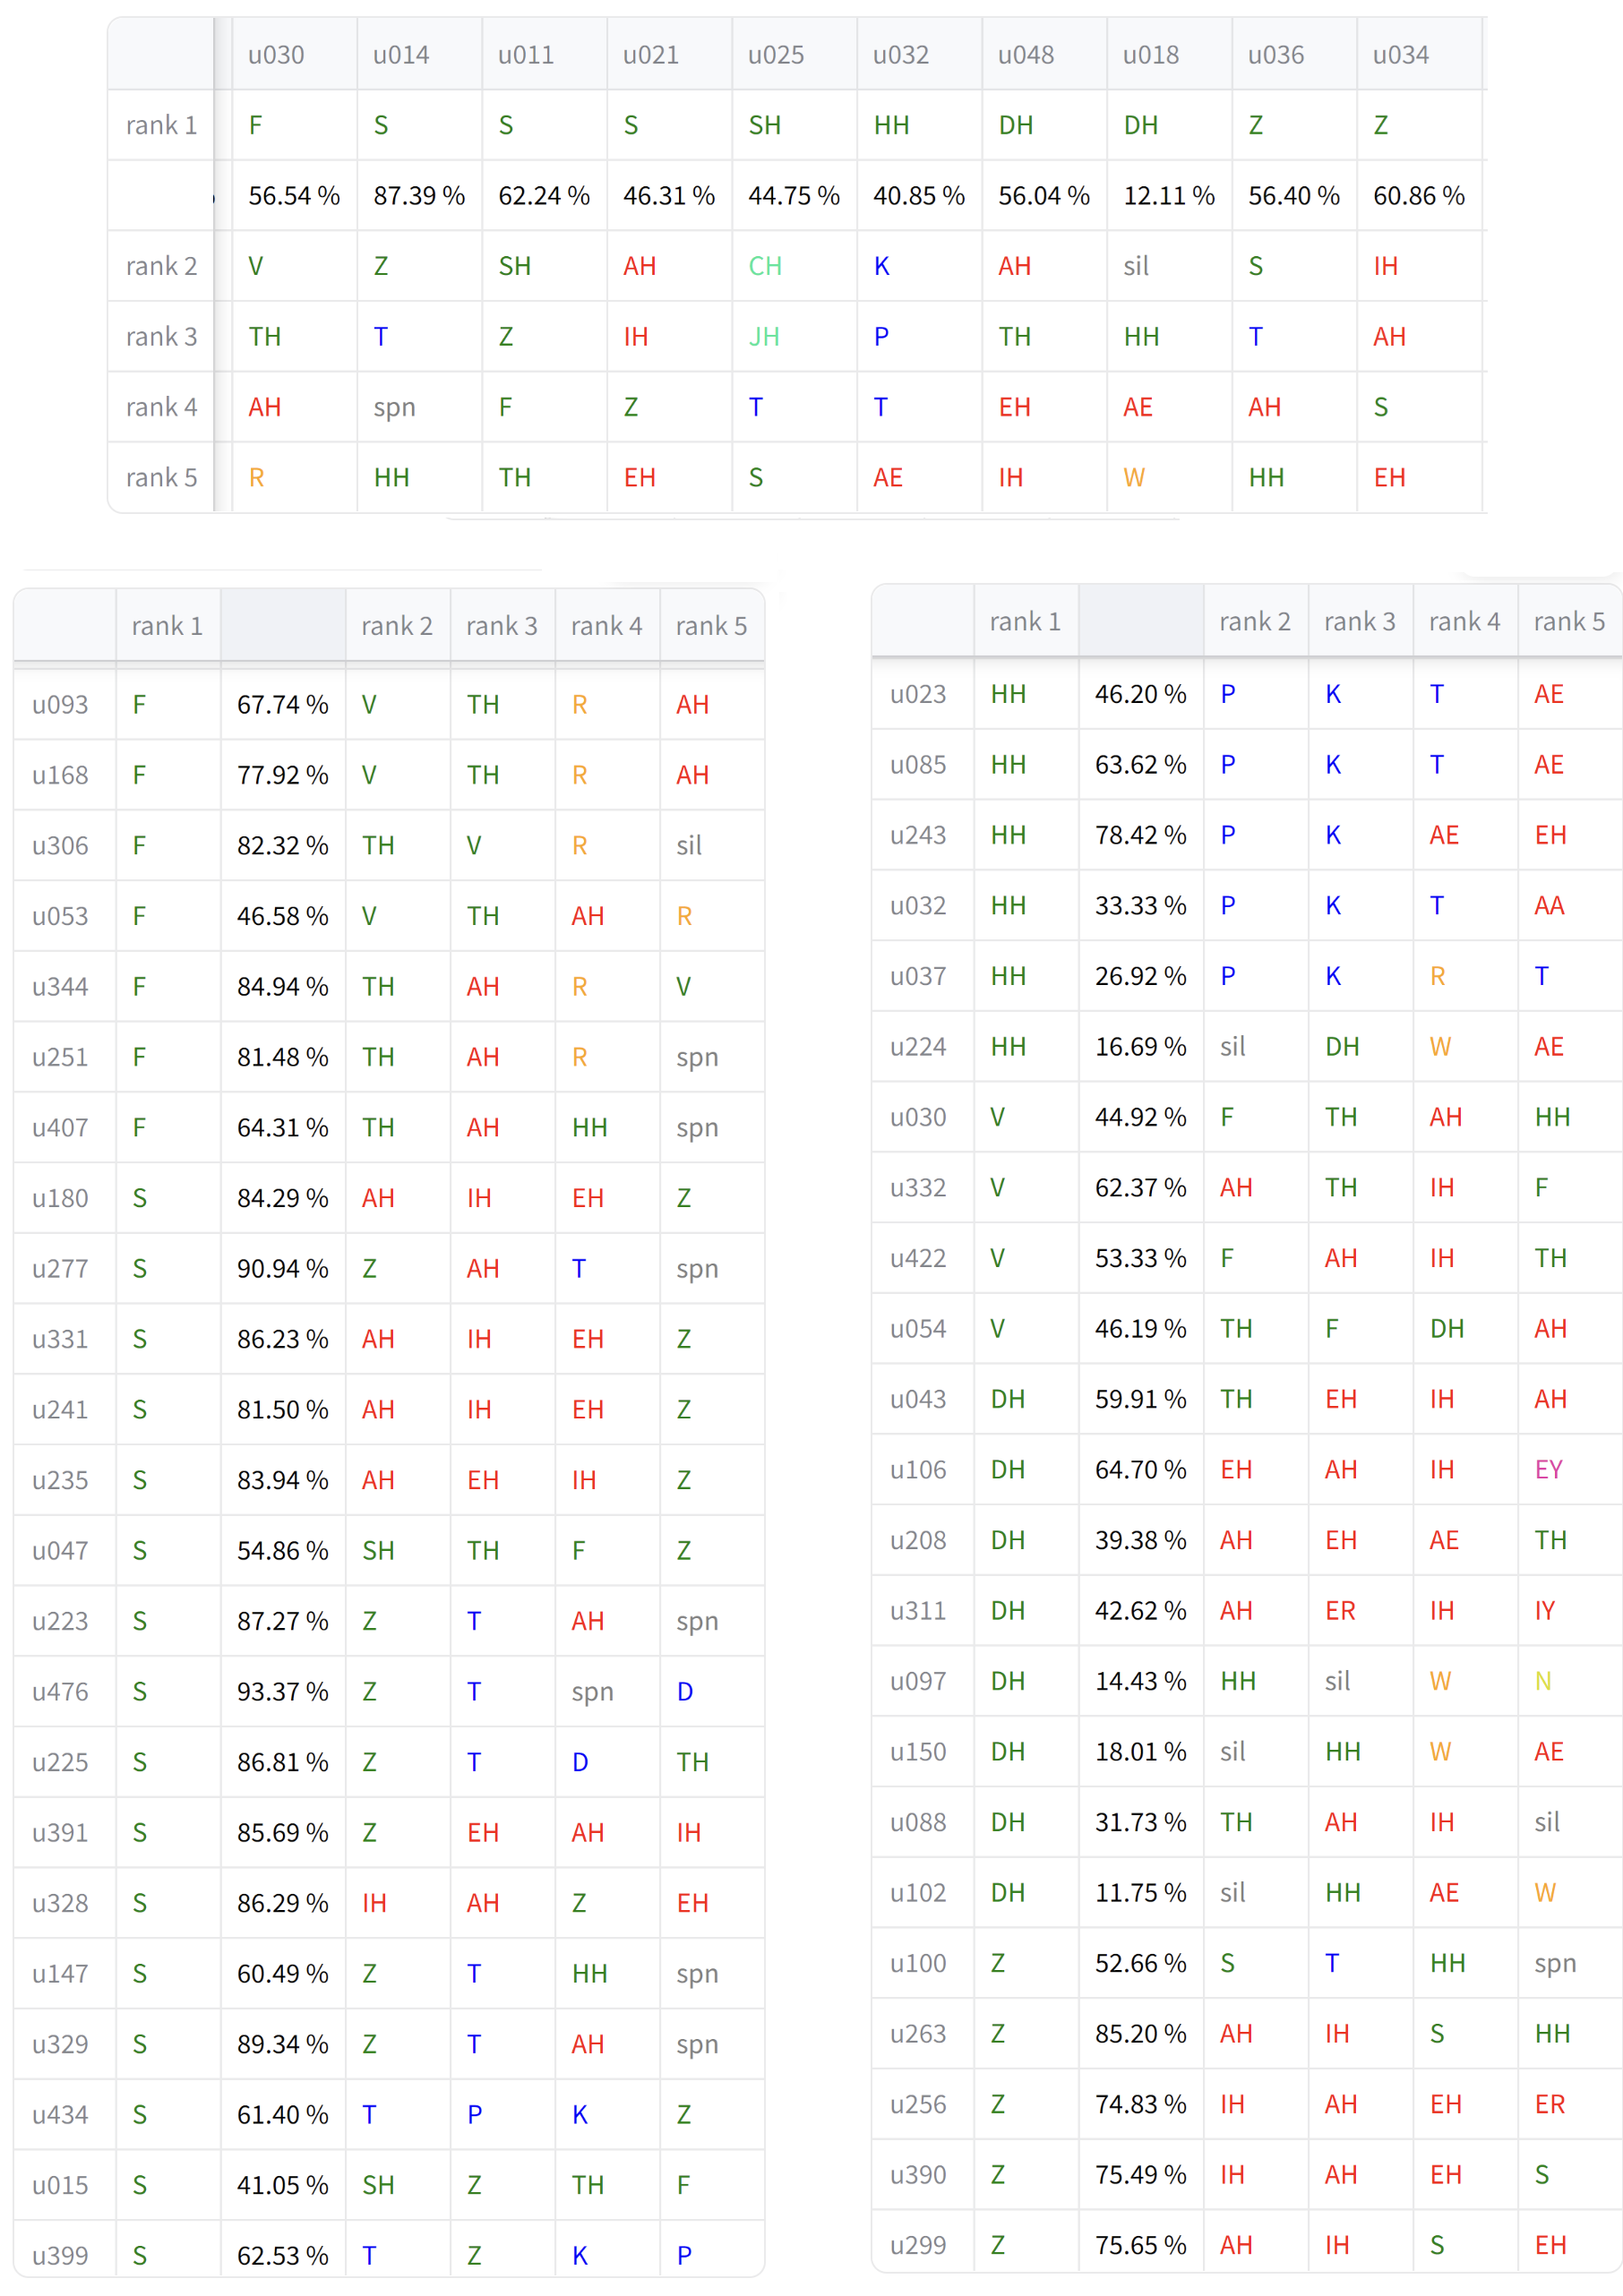
\includegraphics[width=\tempwidth]{figures/ch4figs/fri_phn.png}
             %     \caption{擦音}
             %     \label{fig:hub-u050-ap0500-friobs}
             % \end{subfigure}
             % \vfill
             \begin{subfigure}{\textwidth}
                 \centering
                 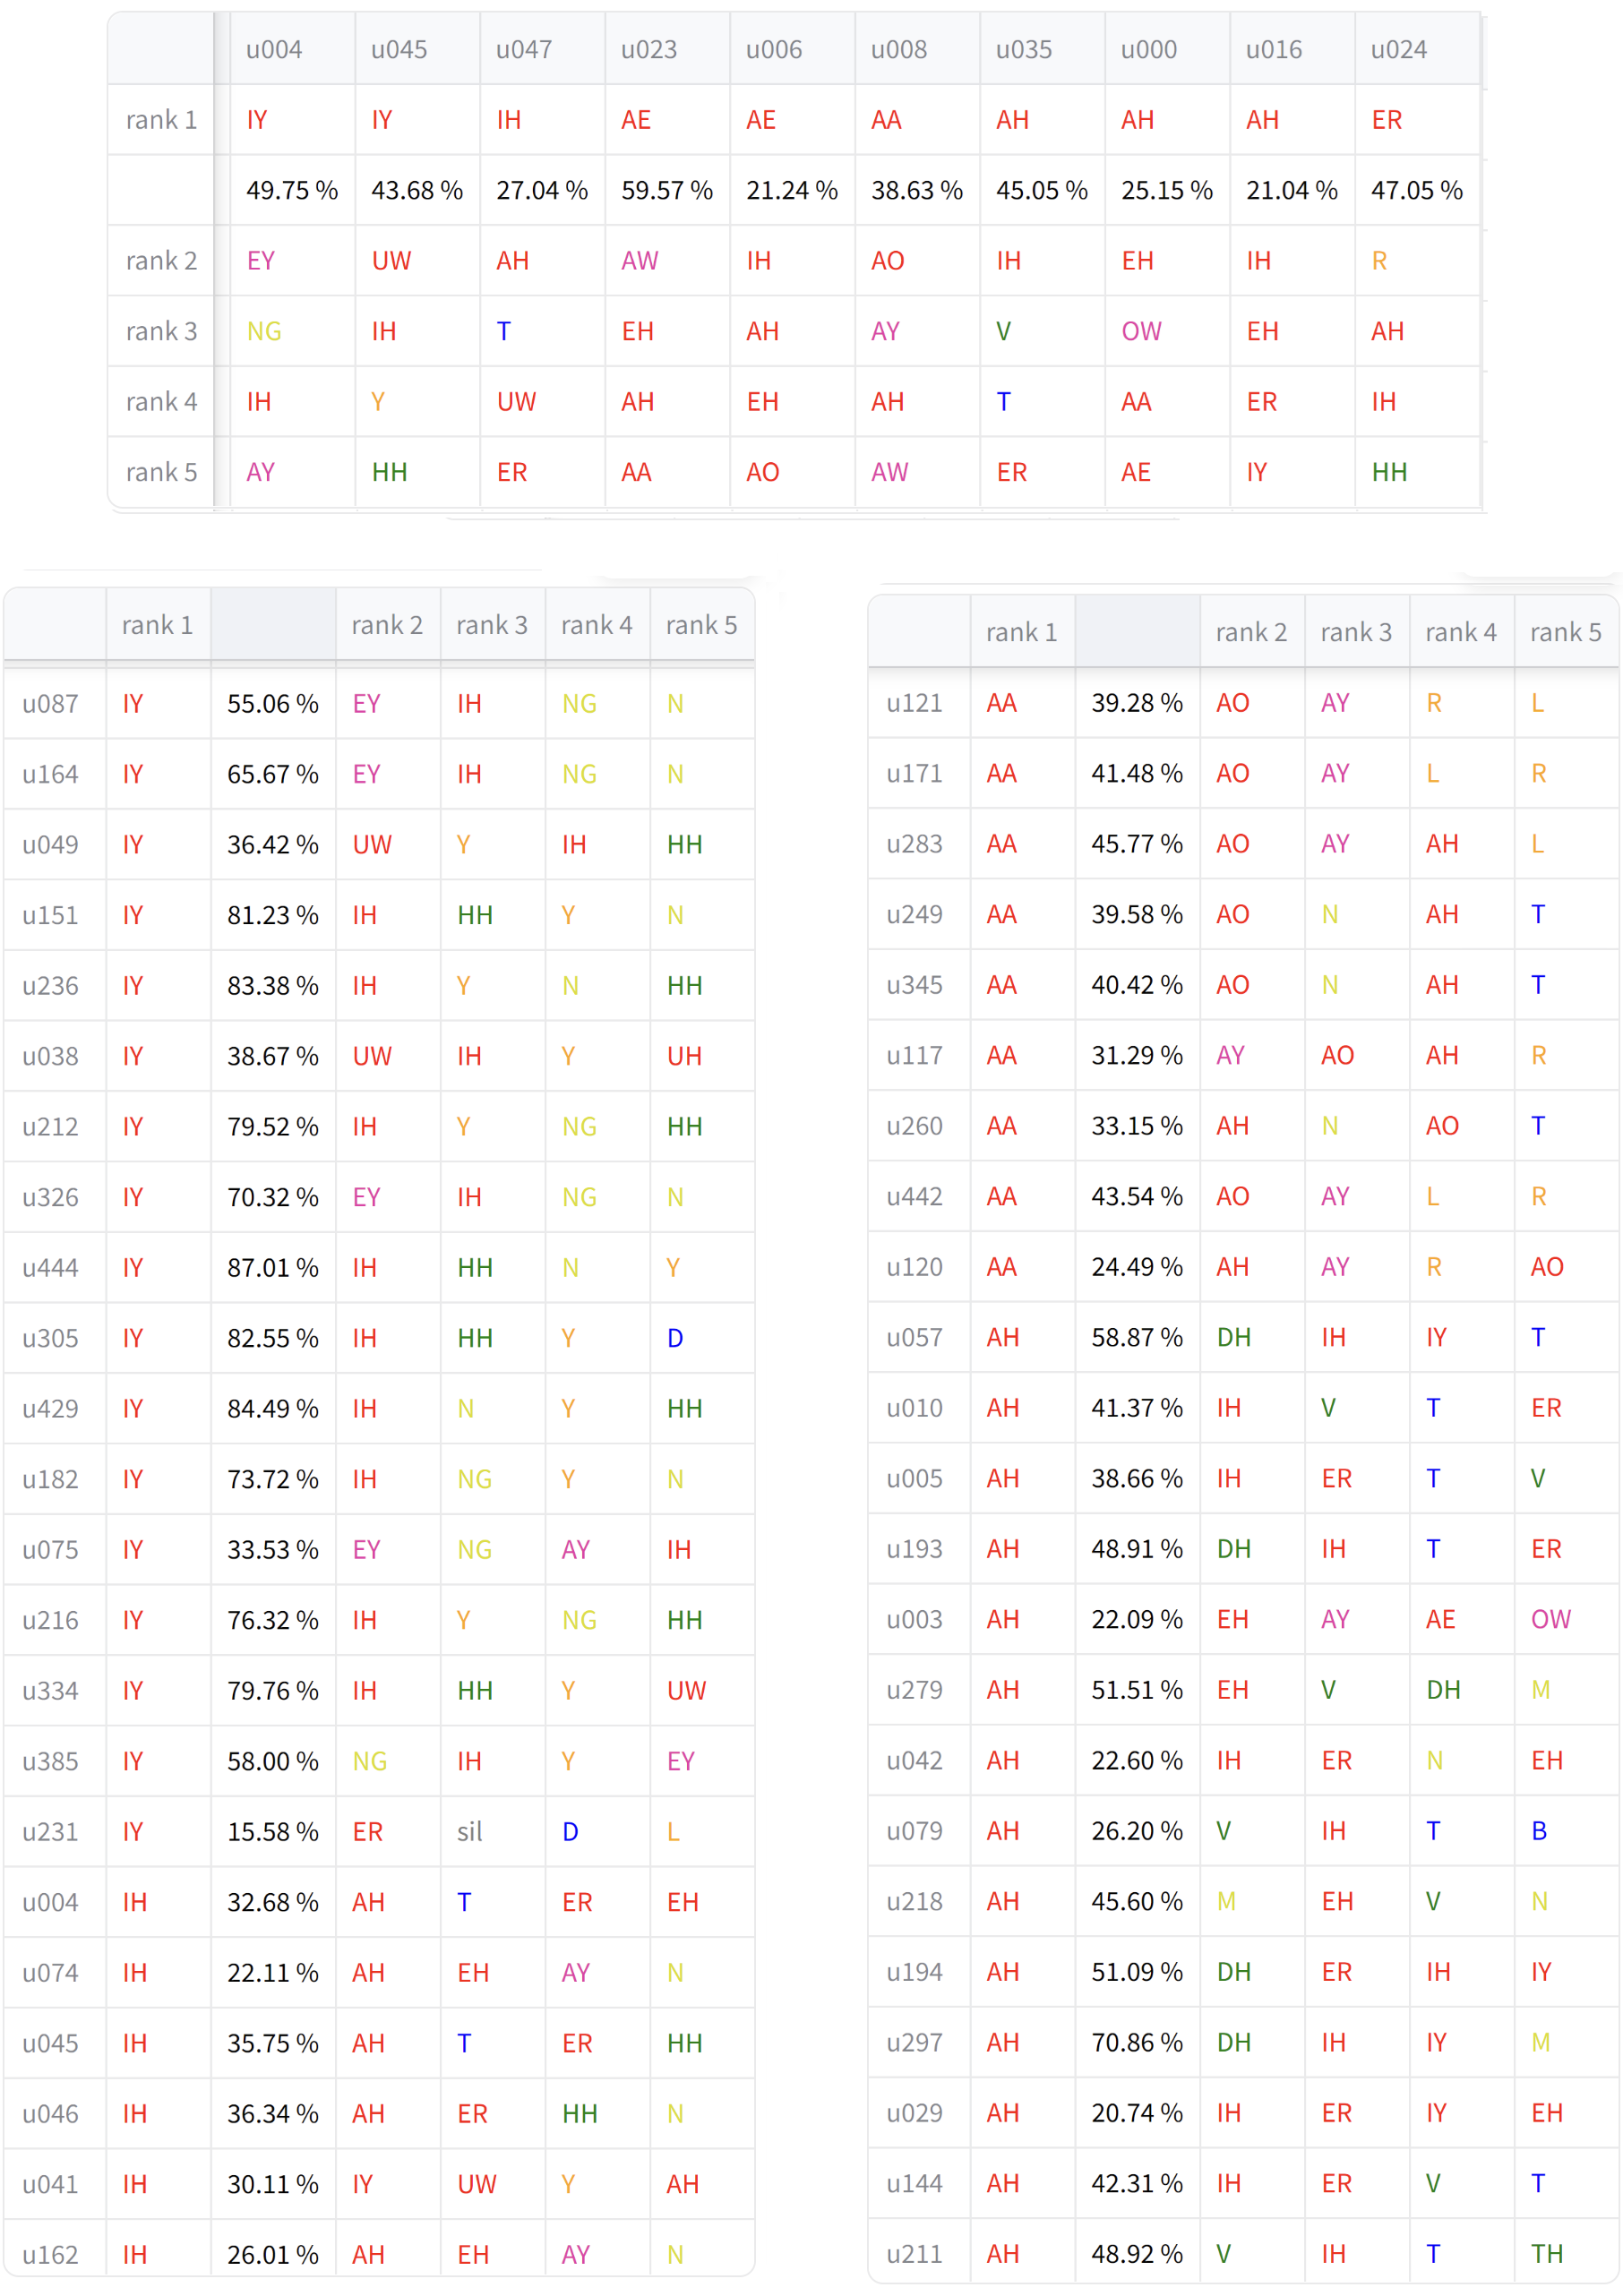
\includegraphics[width=\tempwidth]{figures/ch4figs/vow_phn.png}
                 \caption{單元音}
                 \label{fig:hub-u050-ap0500-vowobs}
             \end{subfigure}

             % \caption{HuBERT 表徵、K-平均演算法分群數 50,比較單一離散單元與使用 500 種次詞單位,}
             % 依據不同音位分類比較符記各自對應的前五高音位
             % (上半部為離散單元,下半部為聲學片段。圖中的百分比為最高機率音位的條件機率 $p_{y|z}(i^*(j)|j)$)
                         \label{fig:hub-u050-phnobserver--3}
        \end{figure}
    }

\subsubsection{聲學片段對應最高機率之音位間的比較}

  接下來,我們比較各個聲學片段與音位之間的對應關係,亦即每個符記所對應最可能的前幾個音位之間,是否依然如離散單元那樣存在特定特徵。觀察以 HuBERT 模型、分群數 50 為基礎,分別以「離散單元」與「500 種次詞單位的聲學片段」為符記的虛擬文字文本,將對應到
塞音、擦音和單元音
部分的次詞單位取出觀察,將每個符記
對應前五高機率的音位排名呈現在
圖 \ref{fig:hub-u050-phnobserver} 中(並附上最高機率音位 $i^*(j)$ 的條件機率值 $p_{y|z}(i^*(j)|j)$),圖中上半部是離散單元,下半部則是聲學片段的結果。
相互比較後可以發現,由於聲學片段的符記數量比離散單元更多,因此在維持對應音位之間相關性的同時,卻能呈現出不同音位間更細節的相關性。例如在圖 \ref{fig:hub-u050-ap0500-ploobs} 中,上半部顯示原先以離散單元為符記時,因為只有 50 種符記,因此只能看出 T、B 與 D 比較容易和哪些其他音位比較相關,但聲學片段卻可以呈現出 P、T、B、D 等更多細節的音位關係。
特別值得注意的是,圖 \ref{fig:aff} 是對應到塞擦音的幾個聲學片段,這些對應到 CH 和 JH 兩種塞擦音的聲學片段也確實給予了同樣是塞擦音的其他音位較高的機率。
    % (aff 圖)
    \begin{figure}
        \centering
        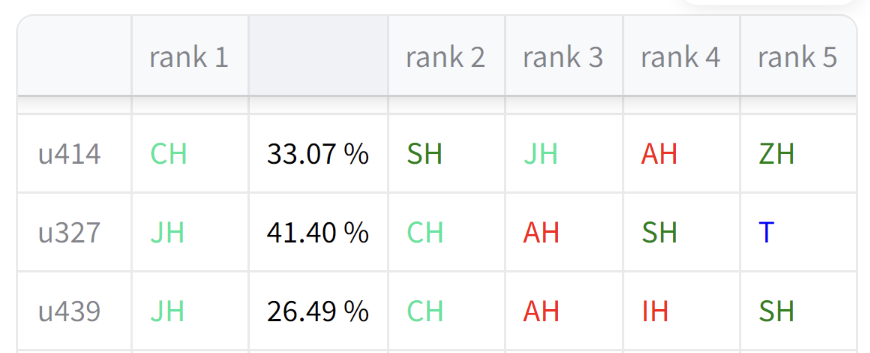
\includegraphics[width=0.8\linewidth]{figures/ch4figs/aff-hub50-500.png}
        \caption{對 HuBERT 分群數 50 離散單元取得 500 種次詞單位後,}
        對應到塞擦音的聲學片段之音位條件機率排名
        \label{fig:aff}
    \end{figure}


\begin{table}[!htbp]
    \centering
    
    \begin{subtable}[t]{\textwidth}
        \centering
        \begin{tabular}{|c|c|c|} \hline 
                符記種數& 音位分類純度& 以音位分類標註之分群純度\\ \hline 
               離散單元&   0.7006&  \textbf{0.1509}
\\ \hline 
                   500    &  0.7116&  0.0340
\\ \hline 
                  1000    &  \textbf{0.7186}&  0.0226
\\ \hline 
                  8000    &  0.7080&  0.0119
\\ \hline 
                 10000    &  0.7048&  0.0113
\\ \hline 
                 20000    &  0.6929&  0.0089\\ \hline 
        \end{tabular}
\caption{群數 = 50}
        \label{tab:ch4-new-hubert-pcls-clu050}
    \end{subtable}        

    \vfill        

    \begin{subtable}[t]{\textwidth}
        \centering
        \begin{tabular}{|c|c|c|} \hline 
                符記種數& 音位分類純度& 以音位分類標註之分群純度\\ \hline 
               離散單元&   \textbf{0.7584}&  \textbf{0.0882}\\ \hline 
                   500    &  0.7578&  0.0326
\\ \hline 
                  1000    &  0.7576&  0.0223
\\ \hline 
                  8000    &  0.7382&  0.0097
\\ \hline 
                 10000    &  0.7346&  0.0090
\\ \hline 
                 20000    &  0.7235&  0.0074
\\ \hline 
        \end{tabular}
\caption{群數 = 100}
        \label{tab:ch4-new-hubert-pcls-clu100}
    \end{subtable}    

\caption{HuBERT 模型在不同詞表大小時的語音學類別分析數據}
    \label{tab:new--hubert-pcls-results}
\end{table}

        仿照第三章,藉由以音位分類作為新的標註計算純度,我們可以確認聲學片段給予同類音位較高機率的效果。然而從表 \ref{tab:new--hubert-pcls-results} 可以發現,隨著符記種數的提升,僅有分群數 50 時在較少符記種類時,音位分類的純度有微幅提升,多數時候符記種數的提高,伴隨的反而是音位分類純度些微的降低。由此可以推斷,次詞單位的引入雖能帶來更多樣的符記,對應音位間的關係卻在 K-平均演算法得到的離散單元已經大致抵定,次詞單位帶來的效果幾乎已經沒什麼改善的空間。
        % \par
其理由很可能是源自次詞單位演算法的特性,聲學片段的計算過程可以把原先代表不同種類音位的離散單元合在一起。因此,即便整體新的符記對應音位的純度有所提升,對音位分類的相關性卻低上不少。  \jcm{phn pur up, but pcls pur down}

\subsection{由音位角度探討}


    {
        \newcommand{\tempwidth}[0]{0.8\linewidth}
        \begin{figure}
             \centering
             \begin{subfigure}{\textwidth}
                 \centering
                 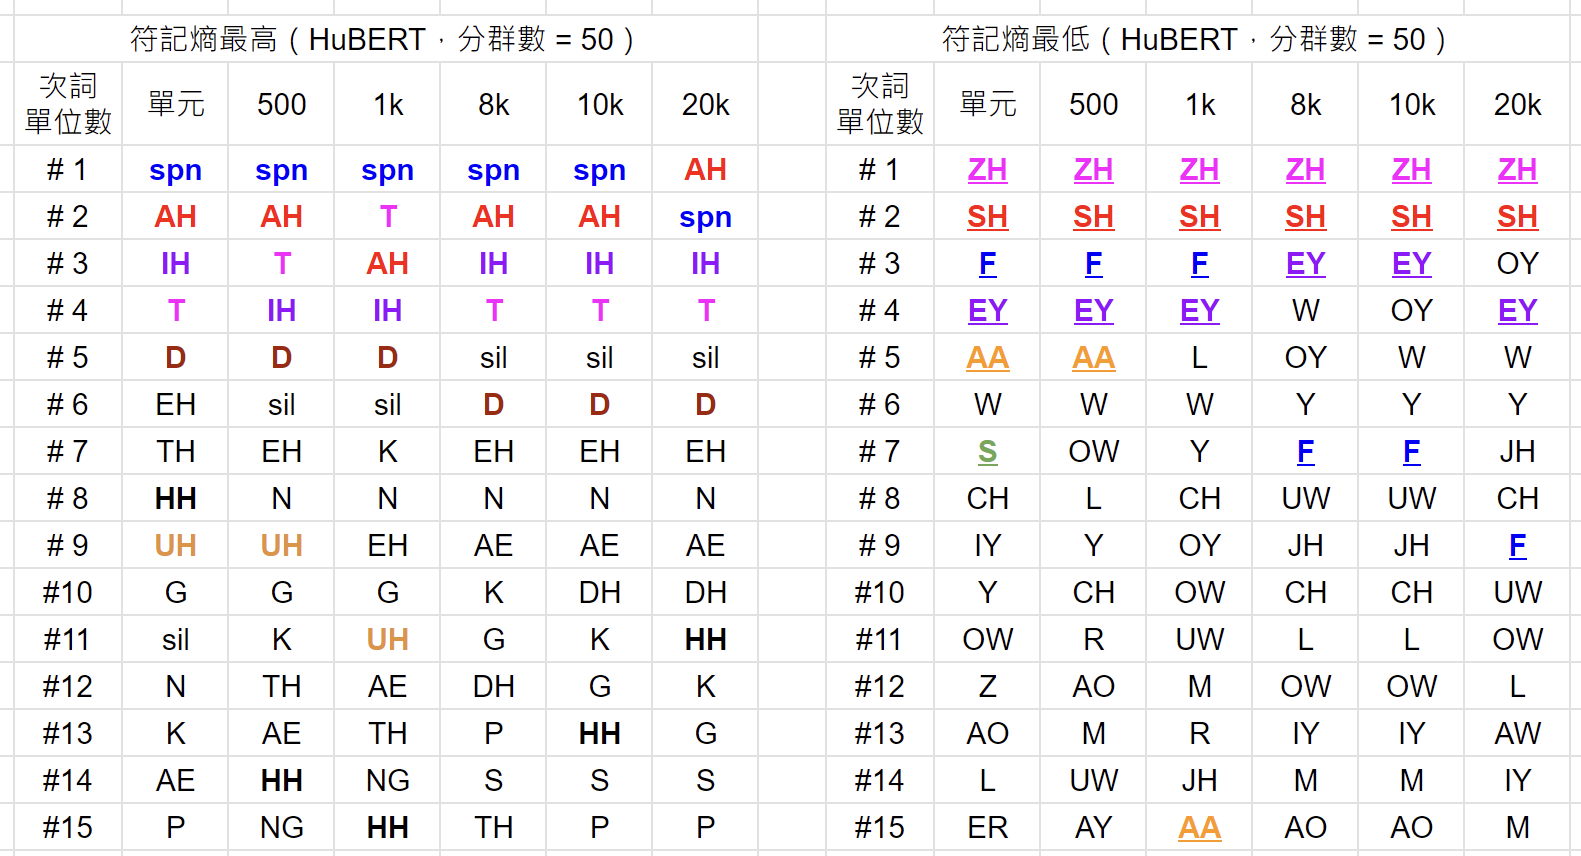
\includegraphics[width=\tempwidth]{figures/ch4figs/phnrank-hub50pcs.png}
                 \caption{分群數 = 50}
                 \label{fig:hub-u050-phnrank-hub50pcs}
             \end{subfigure}
             \vfill
             \begin{subfigure}{\textwidth}
                 \centering
                 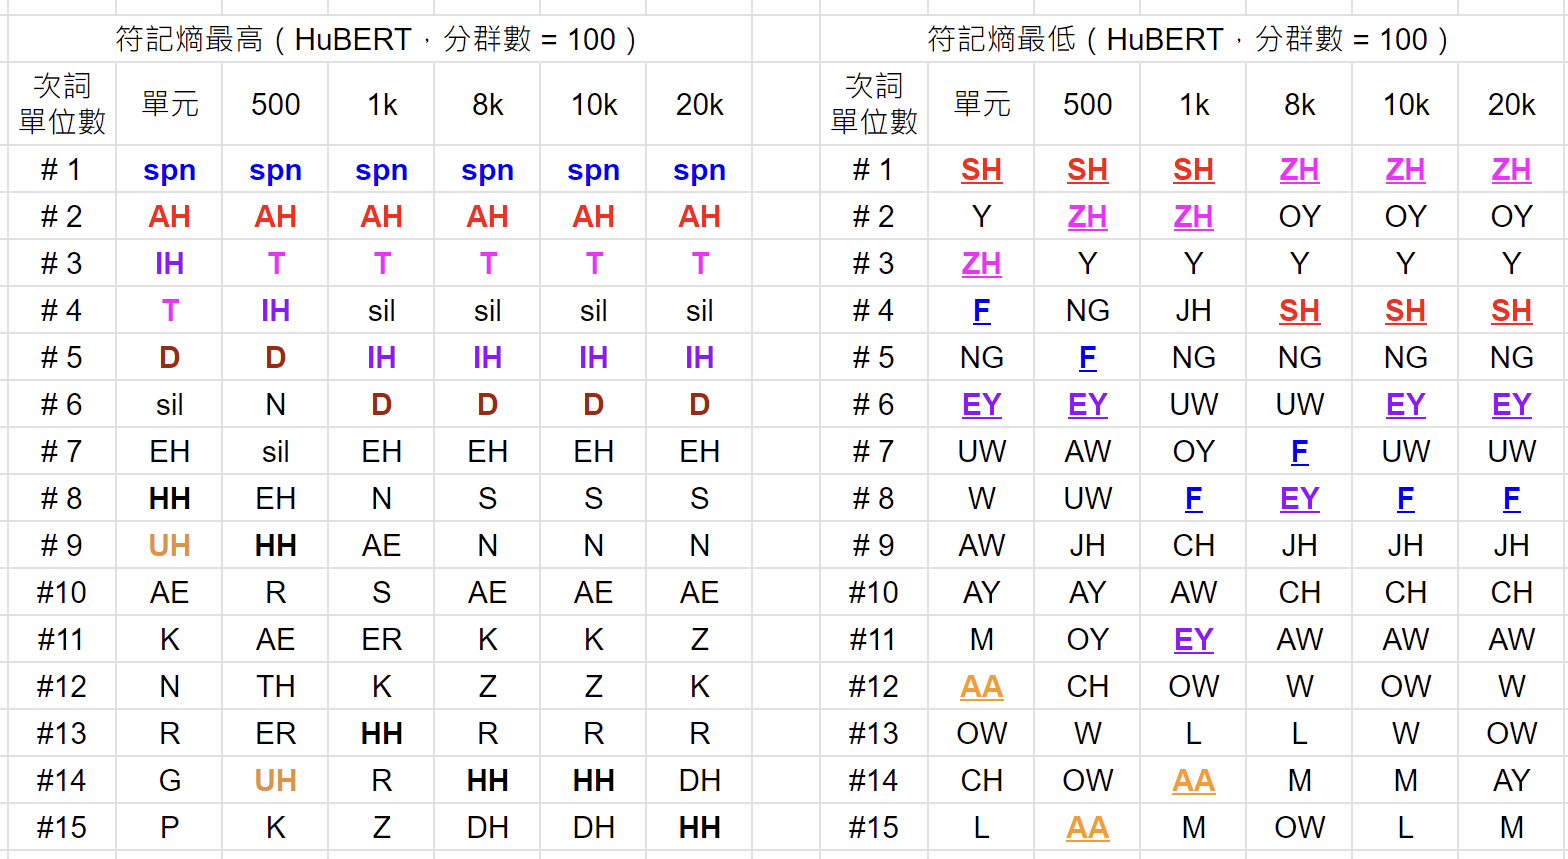
\includegraphics[width=\tempwidth]{figures/ch4figs/phnrank-hub100pcs.png}
                 \caption{分群數 = 100}
                 \label{fig:hub-u050-phnrank-hub100pcs}
             \end{subfigure}

             \caption{HuBERT 表徵、K-平均演算法分群數 50 和 100,}
             比較不同次詞單位種數時,符記熵最高與最低的音位排名
                         \label{fig:hub-u050-phnrank}
        \end{figure}
    }

    
  考慮完聲學片段,接著我們一樣以音位的角度切入,觀察各自音位的符記分佈集中程度。圖 \ref{fig:hub-u050-phnrank} 是對 HuBERT 模型所得的離散單元(比較分群數 50 和 100),以不同次詞單位種數
取得聲學片段後,
對應符記熵 $H(z|y)$ 最高與最低的排名。
比對最左側直行顯示的離散單元排名,亦即第三章不引入次詞單位的結果,可以發現整體排名趨勢雖有些微變動,但對應符記最分散的音位仍以 AH、IH、T、D 為主,而最集中的亦仍然是 ZH、SH、F、EY,與上一章的觀察接近。由此可以推論,音位本身的較容易或較難以歸類的特性,在對語音表徵進行分群時就已經大致呈現;然而,即便聲學片段的演算法允許將代表不同類別音位的離散單元重新組合成新的符記,卻仍舊維持了音位本身分散程度的趨勢。
因此,音位本身對應符記,不論是使用 K-平均演算法離散化獲得,或是以次詞單位重新歸類,這個分散程度的趨勢都是差不多的,音位本身的發音特徵確實是超出單一音框、影響範圍更廣的特性。 




{
\begin{figure}  % 有辦法再改圖
    \centering
    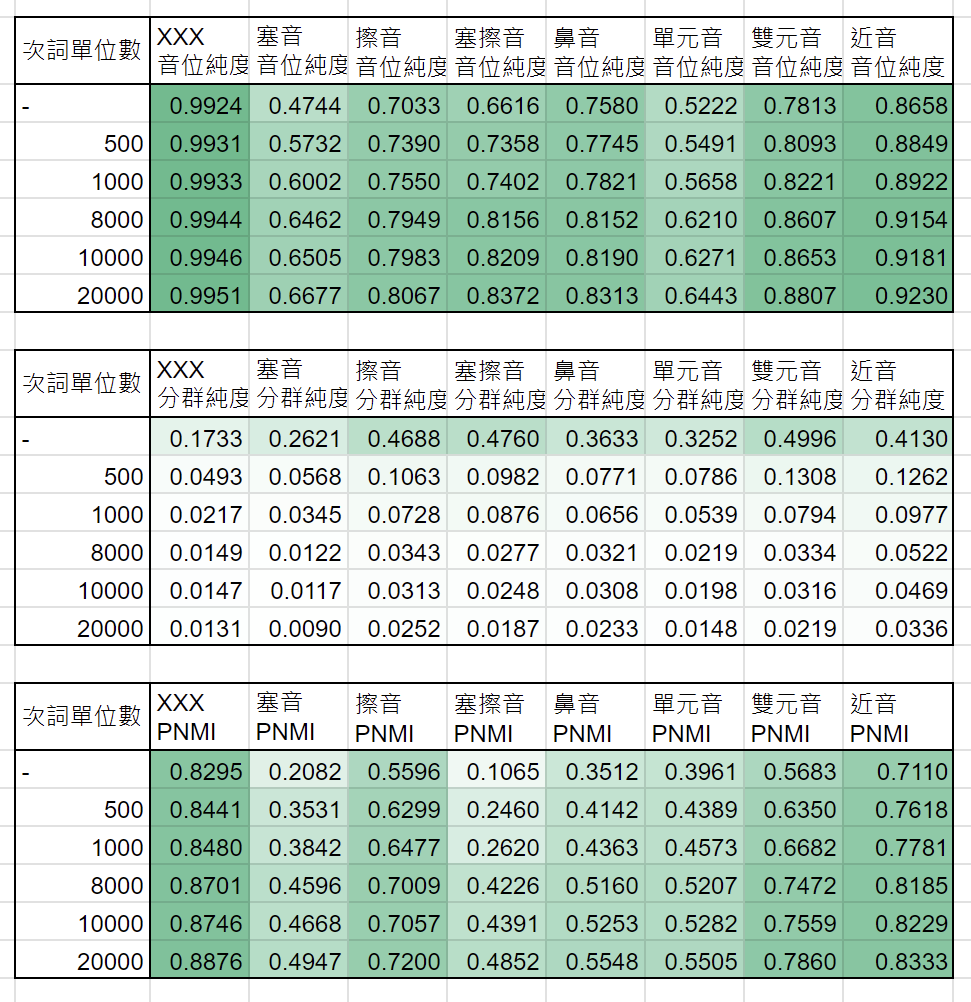
\includegraphics[width=0.6\linewidth]{figures/ch4figs/hub50-ap-detailedpur.png}
    \caption{HuBERT 分群數 50 的離散單元,以不同符記種數取得聲學片段後,}
    按照音位分類分開各自計算的純度與相互資訊
    \label{fig:hub50-ap-detailedpur}
\end{figure}
}


\begin{figure}
    \centering
    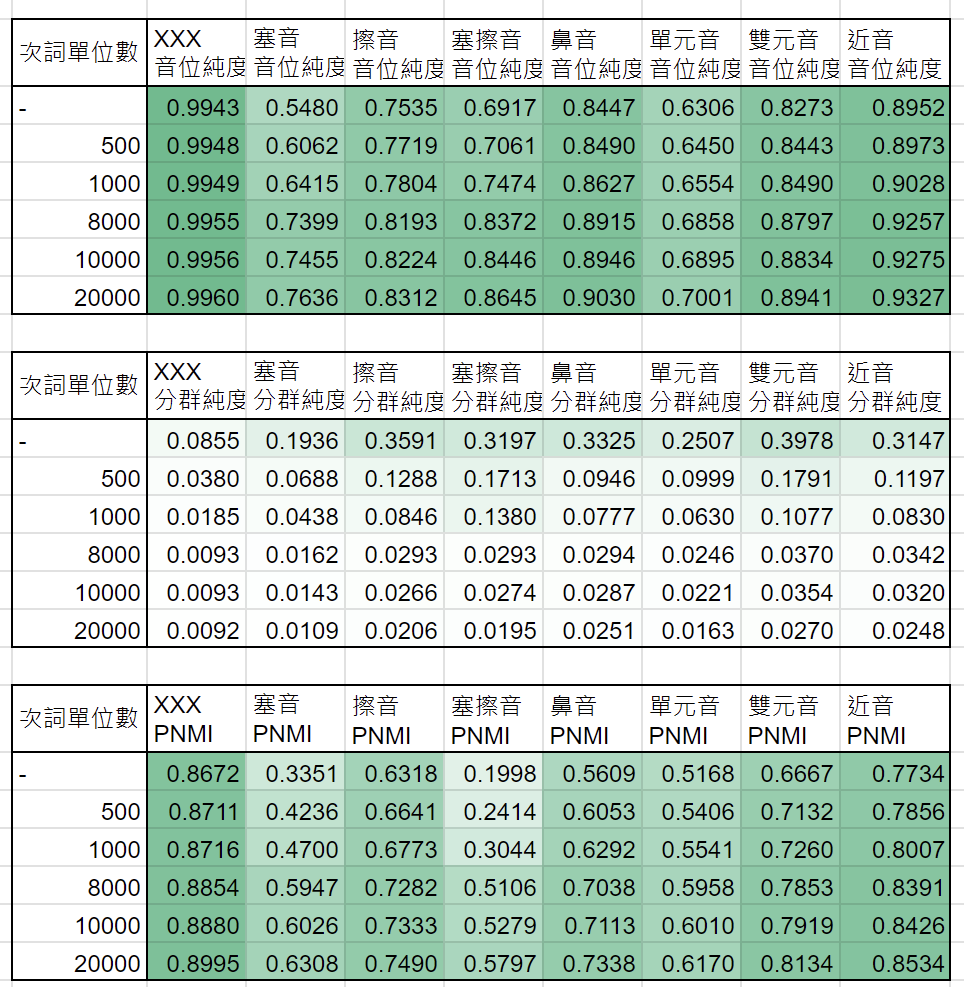
\includegraphics[width=0.6\linewidth]{figures/ch4figs/hub100-ap-detailedpur.png}
     \caption{HuBERT 分群數 100 的離散單元,以不同符記種數取得聲學片段後,}
    按照音位分類分開各自計算的純度與相互資訊
    \label{fig:hub100-ap-detailedpur}
\end{figure}


  
        最後,我們可以將音位分類分別考慮,統計其各自的純度與相互資訊數據,與上一章節比對。對 HuBERT 分群數 50 離散單元文本以不同次詞單位種數處理後,不同音位分類各自的純度與相互資訊數據以圖 \ref{fig:hub50-ap-detailedpur} 呈現。由結果可以發現,隨著次詞單位種數的增加,除了原本音位純度較低的塞音在音位純度與相互資訊的提升較為明顯外,其他音位分類的音位純度與相互資訊就已經較高,因而
雖然增加得不是很明顯,
但整體大致仍然有所改善。比較圖 \ref{fig:hub100-ap-detailedpur},可以確認此一變化在分群數改為 100 時依然可見。


% {

% \begin{figure}
%     \centering
%     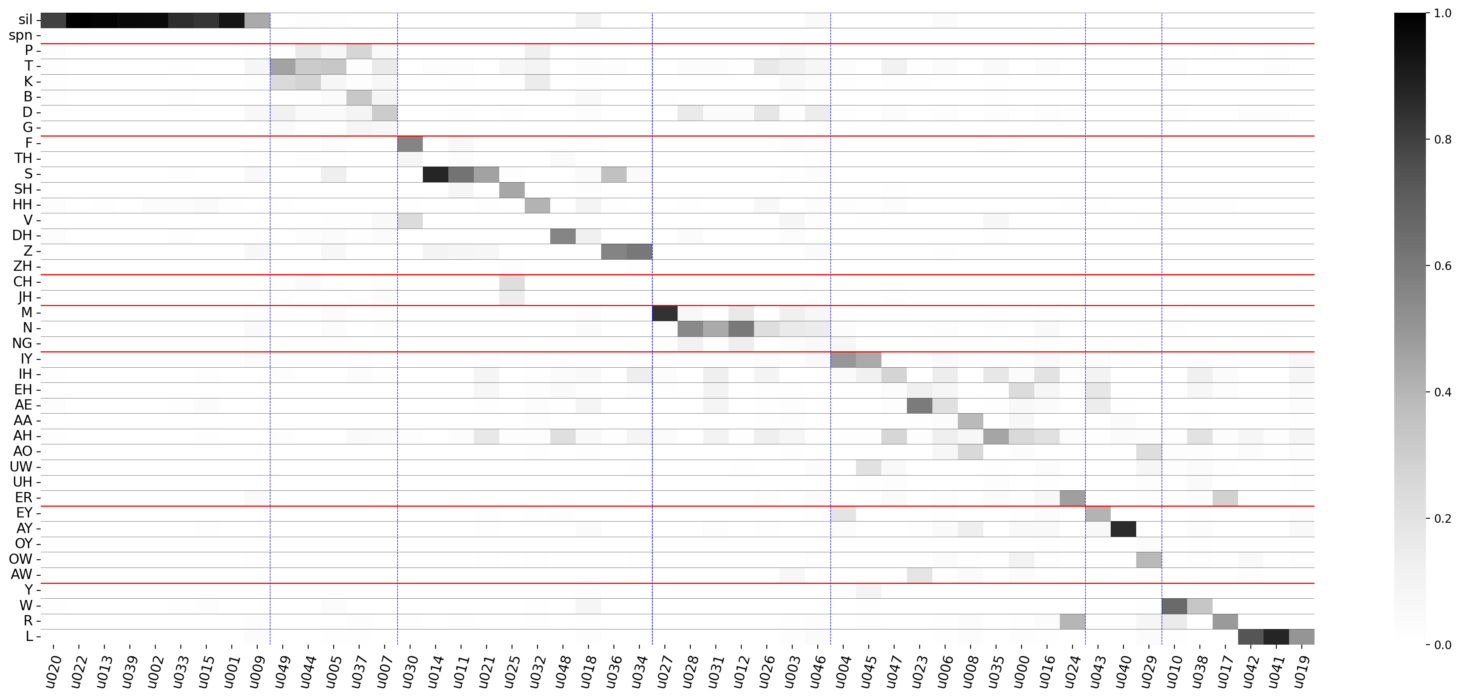
\includegraphics[width=1\linewidth]{figures/ch4figs/hub-u050-ap0000-givenunit-byphn.png}
%     \caption{hub-u050-ap0000-givenunit-byphn}
%     \label{fig:hub-u050-ap0000-givenunit-byphn--detailed}
% \end{figure}

% \begin{figure}
%     \centering
%     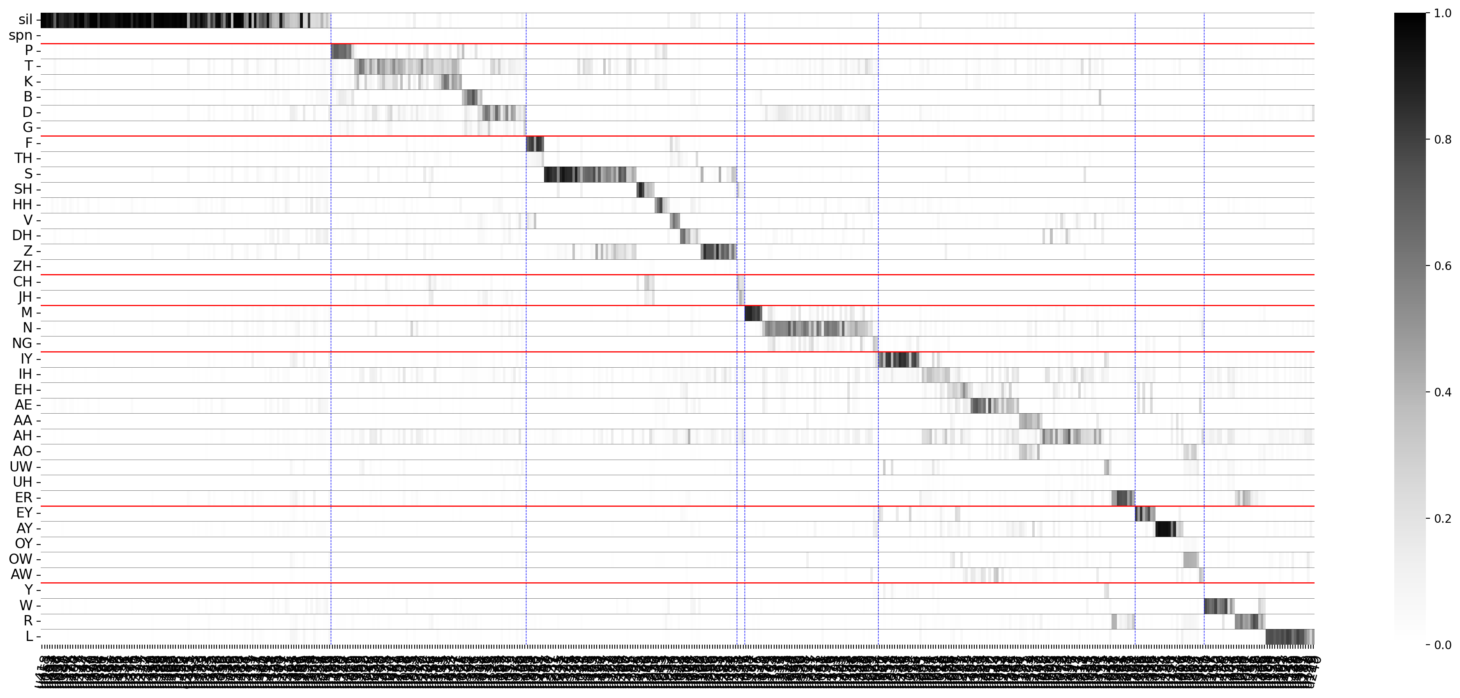
\includegraphics[width=1\linewidth]{figures/ch4figs/hub-u050-ap0500-givenunit-byphn.png}
%     \caption{hub-u050-ap0500-givenunit-byphn}
%     \label{fig:hub-u050-ap0500-givenunit-byphn--detailed}
% \end{figure}

% \begin{figure}
%     \centering
%     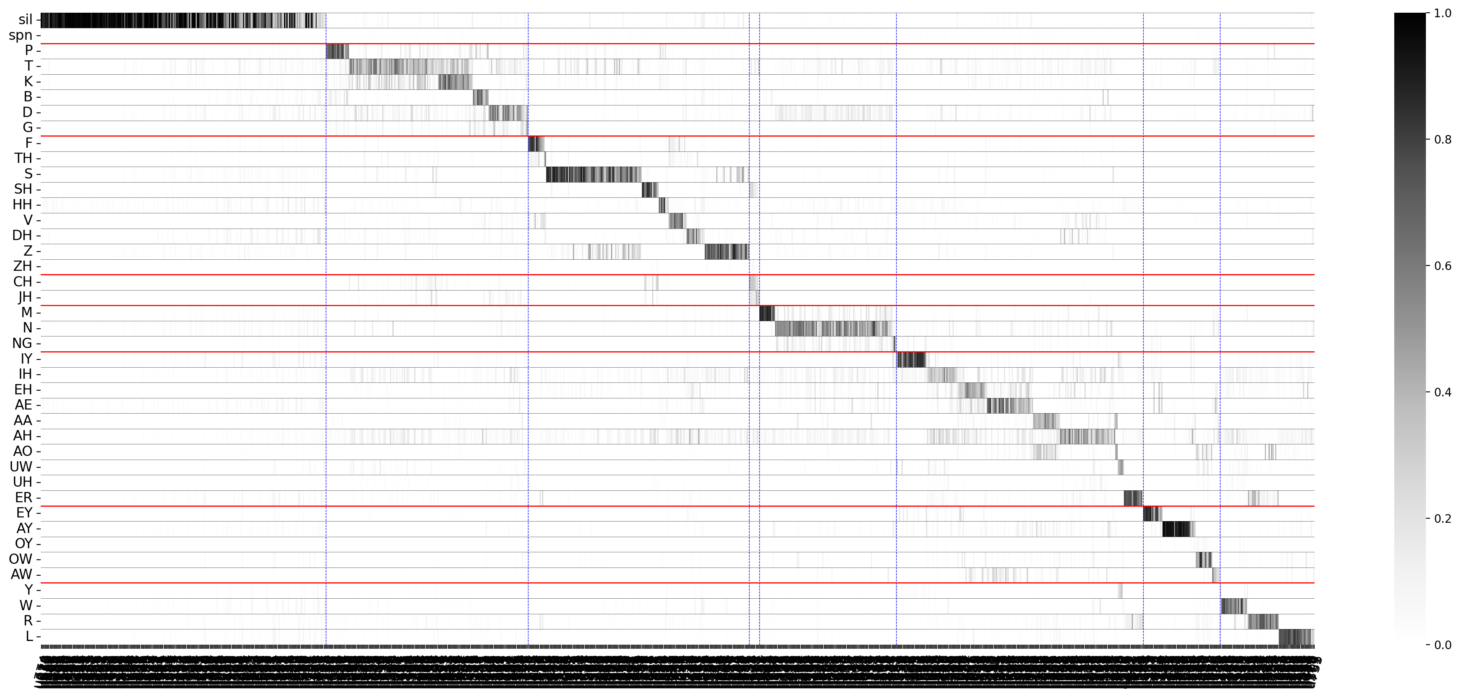
\includegraphics[width=1\linewidth]{figures/ch4figs/hub-u050-ap1000-givenunit-byphn.png}
%     \caption{hub-u050-ap1000-givenunit-byphn}
%     \label{fig:hub-u050-ap1000-givenunit-byphn--detailed}
% \end{figure}

% \begin{figure}
%     \centering
%     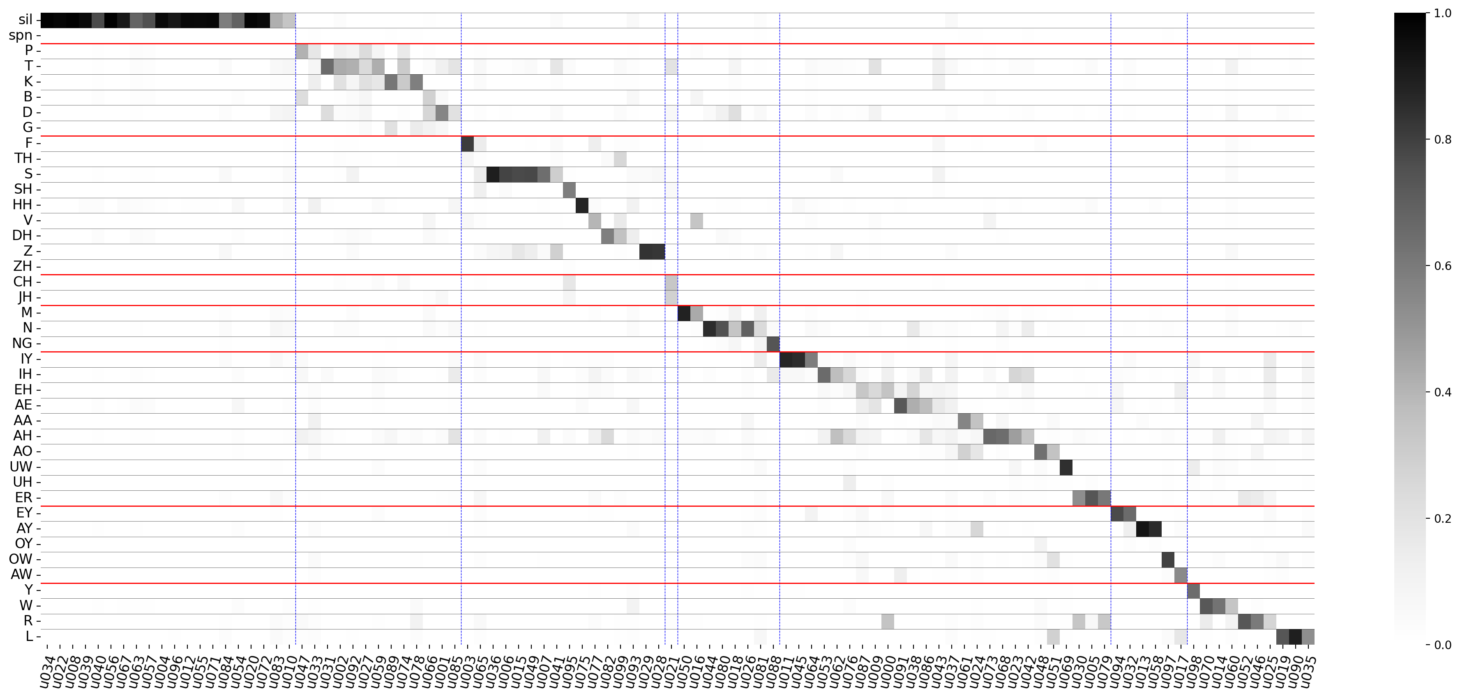
\includegraphics[width=1\linewidth]{figures/ch4figs/hub-u100-ap0000-givenunit-byphn.png}
%     \caption{hub-u100-ap0000-givenunit-byphn}
%     \label{fig:hub-u100-ap0000-givenunit-byphn--detailed}
% \end{figure}
% \begin{figure}
%     \centering
%     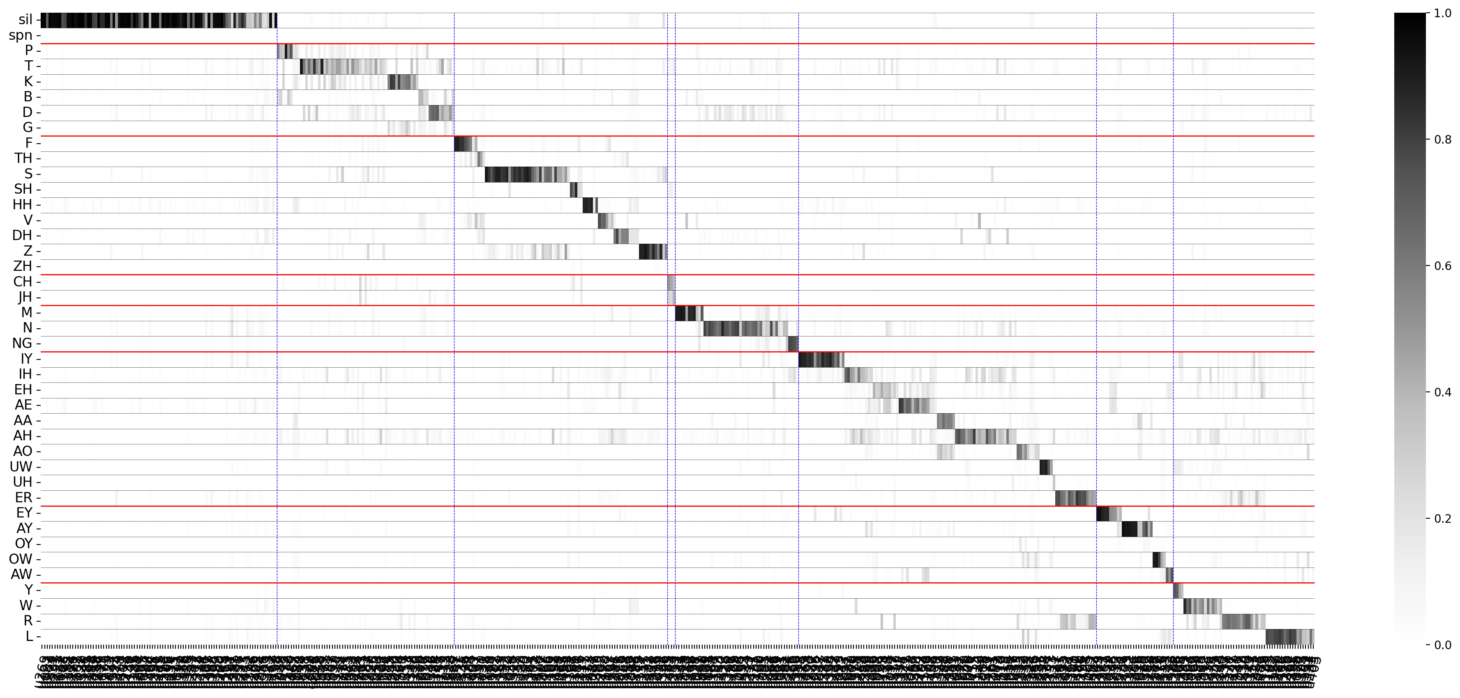
\includegraphics[width=1\linewidth]{figures/ch4figs/hub-u100-ap0500-givenunit-byphn.png}
%     \caption{hub-u100-ap0500-givenunit-byphn}
%     \label{fig:hub-u100-ap0500-givenunit-byphn--detailed}
% \end{figure}
% \begin{figure}
%     \centering
%     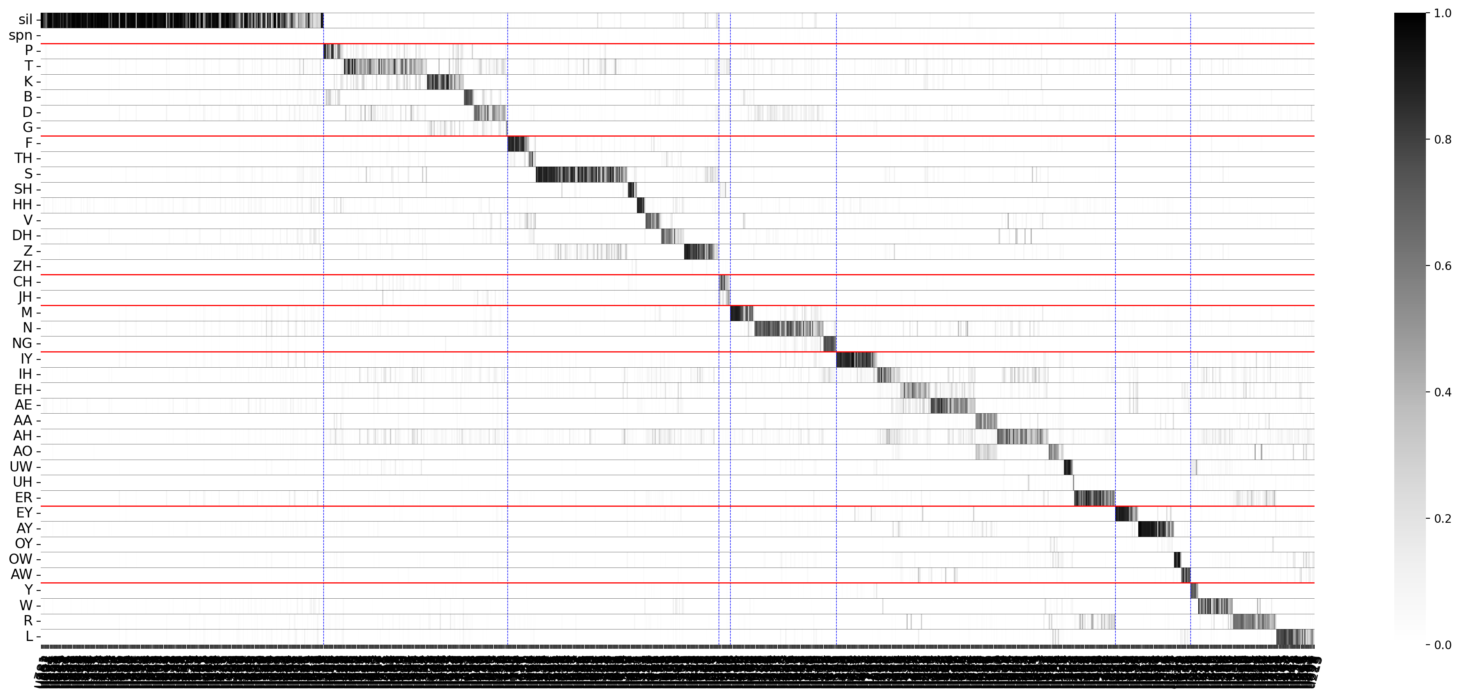
\includegraphics[width=1\linewidth]{figures/ch4figs/hub-u100-ap1000-givenunit-byphn.png}
%     \caption{hub-u100-ap1000-givenunit-byphn}
%     \label{fig:hub-u100-ap1000-givenunit-byphn--detailed}
% \end{figure}
% }  % heatmaps


\jcm{section{分析結果} }
\jcm{  以下數據中的「長度壓縮比率」係指透過分詞方法後,每一個句子的「單詞」數與原先離散單元的數量相比之比值。由於長度壓縮比率是針對離散單元分詞所得到,與標註無關,因此只在音位分析的表格上呈現。}
\jcm{subsection{基於各自音位的分析}}
\jcm{  首先,為了比較不同詞表大小對於純度、相互資訊等數據的影響,先分別固定語音模型為 HuBERT 和 Wav2vec 2.0,在離散單元的分群數量為 50、100、200 三種設定下,觀察詞表大小造成的變化。由 HuBERT (表 \ref{tab:hubert-phn-results-})和 Wav2vec 2.0(表 \ref{tab:w2v2-phn-results})的數據比較可觀察到,詞表大小上升除了使得音位純度提高以外,相互資訊也是隨之提高的,可以發現使用分詞方法並給予足夠大的詞表,對於找出語音中的資訊確實有所幫助。}
\jcm{        接著從另一個角度切入,比較同樣都是離散單元分群數為 200 的條件下,不同語音基石模型的分析數據。由表 \ref{tab:ch4-models-phn} 可以發現,HuBERT 模型在音位純度與相互資訊勝過其他模型,這個結論與上一章節是一致的。}
\jcm{        有趣的是,觀察長度壓縮比率可以發現,CPC 模型在分詞演算法的引入後,能夠使序列變得最短,但同時在音位純度與相互資訊上也有所犧牲;而 HuBERT 雖然在這些分析數據上高過其他三者,卻同時達成了比 Wav2vec 2.0 和 LogMel 更好的壓縮比率。因此綜合看來,這很可能是目前使用語音離散單元進行研究時,HuBERT 模型仍然是領域內首選的緣由。}
\jcm{                
\begin{table}[!htbp]
    \centering
    \begin{subtable}[t]{\textwidth}
        \centering
        \begin{tabular}{|c|c|c|c|c|c|c|} \hline 
                詞表大小  & 音位純度 & 分群純度 & 音位熵 & 離散單元熵 &    PNMI & 長度壓縮比率 \\ \hline 
50 (未分詞)& 0.5256& 0.3382& 3.3152& 3.8681& 0.4993&1.0000\\ \hline 
                   500  &   0.5574   &  0.0829 &   3.3152  &  6.0282 & 0.5357 & 0.3486  \\ \hline %%  1.7758       
                  1000  &   0.5744   &  0.0556 &   3.3152  &  6.6594 & 0.5466 & 0.2992  \\ \hline %%  1.8120       
                  8000  &   0.5957   &  0.0257 &   3.3152  &  8.5192 & 0.5729 & 0.2074  \\ \hline %%  1.8993       
                 10000  &   0.5955   &  0.0238 &   3.3152  &  8.7207 & 0.5750 & 0.2007  \\ \hline %%  1.9063       
                 20000  &   0.5921   &  0.0182 &   3.3152  &  9.3527 & 0.5820 & 0.1819  \\ \hline %%  1.9293       
        \end{tabular}
\caption{群數 = 50}
        \label{tab:ch4-hubert-phn-clu050}
    \end{subtable}        

    \jefftablesep        

    \begin{subtable}[t]{\textwidth}
        \centering
        \begin{tabular}{|c|c|c|c|c|c|c|} \hline 
                詞表大小  & 音位純度 & 分群純度 & 音位熵 & 離散單元熵 &    PNMI & 長度壓縮比率 \\ \hline 
100 (未分詞)& 0.6097& 0.2553& 3.3152& 4.5704& 0.5786&1.0000\\ \hline 
                   500  &   0.6260   &  0.0972 &   3.3152  &  6.0655 & 0.5990 & 0.4432  \\ \hline %%  1.9858       
                  1000  &   0.6372   &  0.0631 &   3.3152  &  6.7181 & 0.6089 & 0.3666  \\ \hline %%  2.0186       
                  8000  &   0.6536   &  0.0237 &   3.3152  &  8.5954 & 0.6308 & 0.2444  \\ \hline %%  2.0912       
                 10000  &   0.6527   &  0.0219 &   3.3152  &  8.7938 & 0.6324 & 0.2357  \\ \hline %%  2.0965       
                 20000  &   0.6490   &  0.0173 &   3.3152  &  9.4123 & 0.6378 & 0.2123  \\ \hline %%  2.1145       
        \end{tabular}
\caption{群數 = 100}
        \label{tab:ch4-hubert-phn-clu100}
    \end{subtable}        

    \jefftablesep        

    \begin{subtable}[t]{\textwidth}
        \centering
        \begin{tabular}{|c|c|c|c|c|c|c|} \hline 
                詞表大小  & 音位純度 & 分群純度 & 音位熵 & 離散單元熵 &    PNMI & 長度壓縮比率 \\ \hline 
200 (未分詞)& 0.6474& 0.1644& 3.3152& 5.2681& 0.6289&1.0000\\ \hline 
                   500  &   0.6471   &  0.0930 &   3.3152  &  6.0986 & 0.6314 & 0.5995  \\ \hline %%  2.0934       
                  1000  &   0.6540   &  0.0558 &   3.3152  &  6.7786 & 0.6382 & 0.4609  \\ \hline %%  2.1156       
                  8000  &   0.6690   &  0.0208 &   3.3152  &  8.6544 & 0.6567 & 0.2874  \\ \hline %%  2.1769       
                 10000  &   0.6693   &  0.0189 &   3.3152  &  8.8535 & 0.6584 & 0.2764  \\ \hline %%  2.1826       
                 20000  &   0.6684   &  0.0144 &   3.3152  &  9.4737 & 0.6636 & 0.2467  \\ \hline %%  2.1999      
        \end{tabular}
\caption{群數 = 200}
        \label{tab:ch4-hubert-phn-clu200}
    \end{subtable}        

\caption{HuBERT 模型在不同詞表大小時的音位分析數據}
    \label{tab:hubert-phn-results}
\end{table}



\begin{table}[!htbp]
    \centering
    \begin{subtable}[t]{\textwidth}
        \centering
        \begin{tabular}{|c|c|c|c|c|c|c|} \hline 
                詞表大小  & 音位純度 & 分群純度 & 音位熵 & 離散單元熵 &    PNMI & 長度壓縮比率 \\ \hline 
 50 (未分詞)&  0.4006 &   0.2676 & 3.3152 &     3.8215 & 0.3706&1.0000\\ \hline 
                  500  &   0.4295&     0.0594    &3.3152 &   6.0328  &       0.4027 &0.3943 \\ \hline %%  
                 1000  &   0.4411&     0.0456    &3.3152 &   6.6250  &       0.4132 &0.3448 \\ \hline %%  
                 8000  &   0.4676&     0.0239    &3.3152 &   8.4954  &       0.4438 &0.2429 \\ \hline %%  
                10000  &   0.4705&     0.0227    &3.3152 &   8.6966  &       0.4477 &0.2352 \\ \hline %%  
                20000  &   0.4753&     0.0185    &3.3152 &   9.3471  &       0.4587 &0.2132 \\ \hline %%  
        \end{tabular}
\caption{群數 = 50}
        \label{tab:ch4-w2v2-phn-clu050}
    \end{subtable}        

    \jefftablesep        

    \begin{subtable}[t]{\textwidth}
        \centering
        \begin{tabular}{|c|c|c|c|c|c|c|} \hline 
                詞表大小  & 音位純度 & 分群純度 & 音位熵 & 離散單元熵 &    PNMI & 長度壓縮比率 \\ \hline 
 100 (未分詞)&0.4877 &   0.2118 & 3.3152 &     4.5284 & 0.4596&1.0000\\ \hline 
                  500  &   0.5016&     0.0697    &3.3152 &   6.0769  &       0.4784 &0.4926 \\ \hline %%  
                 1000  &   0.5108&     0.0444    &3.3152 &   6.7265  &       0.4867 &0.4160 \\ \hline %%  
                 8000  &   0.5427&     0.0215    &3.3152 &   8.5576  &       0.5180 &0.2895 \\ \hline %%  
                10000  &   0.5451&     0.0203    &3.3152 &   8.7602  &       0.5218 &0.2797 \\ \hline %%  
                20000  &   0.5531&     0.0162    &3.3152 &   9.4070  &       0.5345 &0.2526 \\ \hline %%  
        \end{tabular}
\caption{群數 = 100}
        \label{tab:ch4-w2v2-phn-clu100}
    \end{subtable}        

    \jefftablesep        

    \begin{subtable}[t]{\textwidth}
        \centering
        \begin{tabular}{|c|c|c|c|c|c|c|} \hline 
                詞表大小  & 音位純度 & 分群純度 & 音位熵 & 離散單元熵 &    PNMI & 長度壓縮比率 \\ \hline 
 200 (未分詞)&  0.5427 &   0.1467 & 3.3152 &     5.2173 & 0.5188 &1.0000\\ \hline 
                  500  &   0.5481&     0.0846    &3.3152 &   6.0756  &       0.5276 &0.6418 \\ \hline %%  
                 1000  &   0.5549&     0.0509    &3.3152 &   6.7483  &       0.5347 &0.5178 \\ \hline %%  
                 8000  &   0.5803&     0.0180    &3.3152 &   8.6065  &       0.5632 &0.3498 \\ \hline %%  
                10000  &   0.5828&     0.0166    &3.3152 &   8.8136  &       0.5668 &0.3373 \\ \hline %%  
                20000  &   0.5917&     0.0129    &3.3152 &   9.4561  &       0.5794 &0.3026  \\ \hline %%  
        \end{tabular}
\caption{群數 = 200}
        \label{tab:ch4-w2v2-phn-clu200}
    \end{subtable}        

\caption{Wav2vec 2.0 模型在不同詞表大小時的音位分析數據}
    \label{tab:w2v2-phn-results}
\end{table}




\begin{table}[!htbp]
    \centering
    \begin{subtable}[t]{\textwidth}
        \centering
        \begin{tabular}{|c|c|c|c|c|c|c|} \hline 
                詞表大小  & 音位純度 & 分群純度 & 音位熵 & 離散單元熵 &    PNMI & 長度壓縮比率 \\ \hline 
200 (未分詞)&   0.6474 &   0.1644 & 3.3152 &     5.2681 & 0.6289 &1.0000\\ \hline 
                    500   & 0.6471   & 0.0930   & 3.3152 &  6.0986    &  0.6314 &  0.5995  \\ \hline %%   2.0934
                   1000   & 0.6540   & 0.0558   & 3.3152 &  6.7786    &  0.6382 &  0.4609  \\ \hline %%   2.1156
                  10000   & 0.6693   & 0.0189   & 3.3152 &  8.8535    &  0.6584 &  0.2764  \\ \hline %%   2.1826
        \end{tabular}
\caption{HuBERT}
        \label{tab:ch4-phn-model-hubert}
    \end{subtable}        

    \jefftablesep        

    \begin{subtable}[t]{\textwidth}
        \centering
        \begin{tabular}{|c|c|c|c|c|c|c|} \hline 
                詞表大小  & 音位純度 & 分群純度 & 音位熵 & 離散單元熵 &    PNMI & 長度壓縮比率 \\ \hline 
200 (未分詞)&   0.5427 &   0.1467 & 3.3152 &     5.2173 & 0.5188 &1.0000\\ \hline 
                    500   & 0.5481   & 0.0846   & 3.3152 &  6.0756    &  0.5276 &  0.6418  \\ \hline %%   1.7491
                   1000   & 0.5549   & 0.0509   & 3.3152 &  6.7483    &  0.5347 &  0.5178  \\ \hline %%   1.7727
                  10000   & 0.5828   & 0.0166   & 3.3152 &  8.8136    &  0.5668 &  0.3373  \\ \hline %%   1.8791
        \end{tabular}
\caption{Wav2vec 2.0}
        \label{tab:ch4-phn-model-w2v2}
    \end{subtable}        

    
    \jefftablesep        

    \begin{subtable}[t]{\textwidth}
        \centering
        \begin{tabular}{|c|c|c|c|c|c|c|} \hline 
                詞表大小  & 音位純度 & 分群純度 & 音位熵 & 離散單元熵 &    PNMI & 長度壓縮比率 \\ \hline 
200 (未分詞)&   0.6098 &   0.1789 & 3.3146 &     5.1885 & 0.5882 &1.0000\\ \hline 
                    500   & 0.6116   & 0.1048   & 3.3146 &  6.0343    &  0.5936 &  0.4951  \\ \hline %%   1.9677
                   1000   & 0.6134   & 0.0618   & 3.3146 &  6.7245    &  0.5979 &  0.3523  \\ \hline %%   1.9818
                  10000   & 0.6198   & 0.0171   & 3.3146 &  8.8593    &  0.6118 &  0.2061  \\ \hline %%   2.0277
        \end{tabular}
\caption{CPC}
        \label{tab:ch4-phn-model-cpc}
    \end{subtable}        

    \jefftablesep        

    \begin{subtable}[t]{\textwidth}
        \centering
        \begin{tabular}{|c|c|c|c|c|c|c|} \hline 
                詞表大小  & 音位純度 & 分群純度 & 音位熵 & 離散單元熵 &    PNMI & 長度壓縮比率 \\ \hline 
200 (未分詞)&   0.3474 &   0.0569 & 3.3158 &     5.2322 & 0.2955 &1.0000\\ \hline 
                    500   & 0.3515   & 0.0403   & 3.3158 &  6.1035    &  0.3066 &  0.6304  \\ \hline %%   1.0166
                   1000   & 0.3547   & 0.0228   & 3.3158 &  6.7602    &  0.3129 &  0.5185  \\ \hline %%   1.0376
                  10000   & 0.3699   & 0.0121   & 3.3158 &  8.7579    &  0.3381 &  0.3427  \\ \hline %%   1.1211
        \end{tabular}
\caption{LogMel}
        \label{tab:ch4-phn-model-logmel}
    \end{subtable}        

\caption{固定離散單元群數皆為 200,不同基石模型的音位分析數據}
    \label{tab:ch4-models-phn}
\end{table}
}
\jcm{subsection{基於語音學分類的分析}}
\jcm{  最後觀察將語音標註換成語音學分類的結果,一樣可以從表 \ref{tab:hubert-pcls-results}、\ref{tab:w2v2-pcls-results} 和 \ref{tab:ch4-models-pcls} 觀察到與上一小節相同的趨勢。}
\jcm{                
        \begin{table}[!htbp]
            \centering
            \begin{subtable}[t]{\textwidth}
                \centering
                \begin{tabular}{|c|c|c|c|c|c|} \hline 
                        詞表大小  & 標註純度 & 分群純度 & 標註熵 & 離散單元熵 &     NMI   \\ \hline 
                       50 (未分詞)&   0.7466  &  0.1422 & 1.7530 &   3.8681 &  0.5742 \\ \hline 
                           500    &  0.7510  &  0.0345  & 1.7530 &  6.0282  &     0.5789  \\ \hline 
                          1000    &  0.7492  &  0.0225  & 1.7530 &  6.6594  &     0.5756  \\ \hline 
                          8000    &  0.7288  &  0.0116  & 1.7530 &  8.5192  &     0.5630  \\ \hline 
                         10000    &  0.7248  &  0.0110  & 1.7530 &  8.7207  &     0.5606  \\ \hline 
                         20000    &  0.7109  &  0.0089  & 1.7530 &  9.3527  &     0.5537  \\ \hline 
                \end{tabular}
\caption{群數 = 50}
                \label{tab:ch4-hubert-pcls-clu050}
            \end{subtable}        

            \jefftablesep        

            \begin{subtable}[t]{\textwidth}
                \centering
                \begin{tabular}{|c|c|c|c|c|c|} \hline 
                        詞表大小  & 標註純度 & 分群純度 & 標註熵 & 離散單元熵 &     NMI   \\ \hline 
 100 (未分詞)&              0.7804 &   0.0856 &         1.7530 &     4.5704 &  0.6148\\ \hline 
                           500    &  0.7787  &  0.0300  & 1.7530 &  6.0655  &     0.6178  \\ \hline 
                          1000    &  0.7751  &  0.0210  & 1.7530 &  6.7181  &     0.6176  \\ \hline 
                          8000    &  0.7507  &  0.0095  & 1.7530 &  8.5954  &     0.6030  \\ \hline 
                         10000    &  0.7468  &  0.0087  & 1.7530 &  8.7938  &     0.6008  \\ \hline 
                         20000    &  0.7347  &  0.0072  & 1.7530 &  9.4123  &     0.5943  \\ \hline 
                \end{tabular}
\caption{群數 = 100}
                \label{tab:ch4-hubert-pcls-clu100}
            \end{subtable}        

            \jefftablesep        

            \begin{subtable}[t]{\textwidth}
                \centering
                \begin{tabular}{|c|c|c|c|c|c|} \hline 
                        詞表大小  & 標註純度 & 分群純度 & 標註熵 & 離散單元熵 &     NMI   \\ \hline 
 200 (未分詞)&              0.8004 &   0.0464 &         1.7530 &     5.2681 &  0.6563\\ \hline 
                           500    &  0.7875  &  0.0269  & 1.7530 &  6.0986  &     0.6469  \\ \hline 
                          1000    &  0.7788  &  0.0170  & 1.7530 &  6.7786  &     0.6385  \\ \hline 
                          8000    &  0.7625  &  0.0071  & 1.7530 &  8.6544  &     0.6266  \\ \hline 
                         10000    &  0.7601  &  0.0064  & 1.7530 &  8.8535  &     0.6251  \\ \hline 
                         20000    &  0.7514  &  0.0051  & 1.7530 &  9.4737  &     0.6200   \\ \hline
                \end{tabular}
\caption{群數 = 200}
                \label{tab:ch4-hubert-pcls-clu200}
            \end{subtable}        

\caption{HuBERT 模型在不同詞表大小時的語音學類別分析數據}
            \label{tab:hubert-pcls-results}
        \end{table}

\begin{table}[!htbp]
    \centering
    \begin{subtable}[t]{\textwidth}
        \centering
        \begin{tabular}{|c|c|c|c|c|c|} \hline 
                詞表大小 & 標註純度 & 分群純度 & 標註熵 & 離散單元熵 &     NMI \\ \hline 
 50 (未分詞)&      0.6913 &   0.1570 &         1.7530 &     3.8215 &  0.4682\\ \hline 
                  500  &  0.7018 &    0.0339 &   1.7530 &   6.0328 &       0.4873  \\ \hline 
                 1000  &  0.7058 &    0.0273 &   1.7530 &   6.6250 &       0.4913  \\ \hline 
                 8000  &  0.7041 &    0.0158 &   1.7530 &   8.4954 &       0.4956  \\ \hline 
                10000  &  0.7033 &    0.0152 &   1.7530 &   8.6966 &       0.4963  \\ \hline 
                20000  &  0.6961 &    0.0128 &   1.7530 &   9.3471 &       0.4954  \\ \hline 
        \end{tabular}
\caption{群數 = 50}
        \label{tab:ch4-w2v2-pcls-clu050}
    \end{subtable}        

    \jefftablesep        

    \begin{subtable}[t]{\textwidth}
        \centering
        \begin{tabular}{|c|c|c|c|c|c|} \hline 
                詞表大小 & 標註純度 & 分群純度 & 標註熵 & 離散單元熵 &     NMI \\ \hline 
 100 (未分詞)&     0.7219 &   0.0889 &         1.7530 &     4.5284 &  0.5252 \\ \hline 
                  500  &  0.7142 &    0.0288 &   1.7530 &   6.0769 &       0.5297  \\ \hline 
                 1000  &  0.7132 &    0.0197 &   1.7530 &   6.7265 &       0.5294  \\ \hline 
                 8000  &  0.7173 &    0.0108 &   1.7530 &   8.5576 &       0.5352  \\ \hline 
                10000  &  0.7171 &    0.0105 &   1.7530 &   8.7602 &       0.5360  \\ \hline 
                20000  &  0.7149 &    0.0089 &   1.7530 &   9.4070 &       0.5379  \\ \hline 
        \end{tabular}
\caption{群數 = 100}
        \label{tab:ch4-w2v2-pcls-clu100}
    \end{subtable}        

    \jefftablesep        

    \begin{subtable}[t]{\textwidth}
        \centering
        \begin{tabular}{|c|c|c|c|c|c|} \hline 
                詞表大小 & 標註純度 & 分群純度 & 標註熵 & 離散單元熵 &     NMI \\ \hline 
  200 (未分詞)&     0.7490 &   0.0527 &         1.7530 &     5.2173 &  0.5671  \\ \hline 
                  500  &  0.7465 &    0.0310 &   1.7530 &   6.0756 &       0.5685  \\ \hline 
                 1000  &  0.7451 &    0.0199 &   1.7530 &   6.7483 &       0.5692  \\ \hline 
                 8000  &  0.7405 &    0.0071 &   1.7530 &   8.6065 &       0.5725  \\ \hline 
                10000  &  0.7399 &    0.0066 &   1.7530 &   8.8136 &       0.5729  \\ \hline 
                20000  &  0.7391 &    0.0055 &   1.7530 &   9.4561 &       0.5757   \\ \hline
        \end{tabular}
\caption{群數 = 200}
        \label{tab:ch4-w2v2-pcls-clu200}
    \end{subtable}        

\caption{Wav2vec 2.0 模型在不同詞表大小時的語音學類別分析數據}
    \label{tab:w2v2-pcls-results}
\end{table}


        \begin{table}[!htbp]
            \centering
            \begin{subtable}[t]{\textwidth}
                \centering
                \begin{tabular}{|c|c|c|c|c|c|} \hline 
                        詞表大小  & 標註純度 & 分群純度 & 標註熵 & 離散單元熵 &     NMI  \\ \hline 
  200 (未分詞)&         0.8004 &   0.0464 &         1.7530 &     5.2681 &  0.6563\\ \hline 
                            500 &  0.7875 &    0.0269 &   1.7530   & 6.0986 &    0.6469 \\ \hline %%   2.0934
                           1000 &  0.7788 &    0.0170 &   1.7530   & 6.7786 &    0.6385 \\ \hline %%   2.1156
                          10000 &  0.7601 &    0.0064 &   1.7530   & 8.8535 &    0.6251 \\ \hline %%   2.1826
                \end{tabular}
\caption{HuBERT}
                \label{tab:ch4-pcls-model-hubert}
            \end{subtable}        

            \jefftablesep        

            \begin{subtable}[t]{\textwidth}
                \centering
                \begin{tabular}{|c|c|c|c|c|c|} \hline 
                        詞表大小  & 標註純度 & 分群純度 & 標註熵 & 離散單元熵 &     NMI  \\ \hline 
  200 (未分詞)&         0.7490 &   0.0527 &         1.7530 &     5.2173 &  0.5671 \\ \hline 
                            500 &  0.7465 &    0.0310 &   1.7530   & 6.0756 &    0.5685 \\ \hline %%   1.7491
                           1000 &  0.7451 &    0.0199 &   1.7530   & 6.7483 &    0.5692 \\ \hline %%   1.7727
                          10000 &  0.7399 &    0.0066 &   1.7530   & 8.8136 &    0.5729 \\ \hline %%   1.8791
                \end{tabular}
\caption{Wav2vec 2.0}
                \label{tab:ch4-pcls-model-w2v2}
            \end{subtable}        

            
            \jefftablesep        

            \begin{subtable}[t]{\textwidth}
                \centering
                \begin{tabular}{|c|c|c|c|c|c|} \hline 
                        詞表大小  & 標註純度 & 分群純度 & 標註熵 & 離散單元熵 &     NMI  \\ \hline 
 200 (未分詞)&         0.7947 &   0.0644 &         1.7530 &     5.1885 &  0.6345 \\ \hline 
                            500 &  0.7925 &    0.0369 &   1.7530   & 6.0343 &    0.6368 \\ \hline %%   1.9677
                           1000 &  0.7882 &    0.0223 &   1.7530   & 6.7245 &    0.6349 \\ \hline %%   1.9818
                          10000 &  0.7609 &    0.0096 &   1.7530   & 8.8593 &    0.6175 \\ \hline %%   2.0277
                \end{tabular}
\caption{CPC}
                \label{tab:ch4-pcls-model-cpc}
            \end{subtable}        

            \jefftablesep        

            \begin{subtable}[t]{\textwidth}
                \centering
                \begin{tabular}{|c|c|c|c|c|c|} \hline 
                詞表大小 & 標註純度 & 分群純度 & 標註熵 & 離散單元熵 &     NMI \\ \hline 
  200 (未分詞)&         0.6107 &   0.0335 &         1.7530 &     5.2322 &  0.3652 \\ \hline 
                            500 &  0.6156 &    0.0247 &   1.7530   & 6.1035 &    0.3801 \\ \hline %%   1.0166
                           1000 &  0.6189 &    0.0137 &   1.7530   & 6.7602 &    0.3875 \\ \hline %%   1.0376
                          10000 &  0.6322 &    0.0096 &   1.7530   & 8.7579 &    0.4085 \\ \hline %%   1.1211
                \end{tabular}
\caption{LogMel}
                \label{tab:ch4-pcls-model-logmel}
            \end{subtable}        

\caption{固定離散單元群數皆為 200,不同基石模型的語音學類別分析數據}
            \label{tab:ch4-models-pcls}
        \end{table}
        
}

\subsection{分析結論}

  藉由改以次詞單位重新組合離散單元得到聲學片段,
% 我們可以發現
% 可以
透過符記種類數量的提升,
聲學片段可以區別出語音訊號中更細節的語音差異,
進而得以提升音位純度與相互資訊等數據,
提高符記與音位之間的相關性。
同時,
次詞單位的特性雖然允許
對應到不同音位的離散單元重新組合,
然而如此產生的新符記
,
每個音位對應符記的集中或分散程度卻
% 卻在對應的音位分佈卻
% 不太有
差異不大。
因此,
透過將次詞單位應用在離散單元的嘗試,
結合多個離散單元重新編碼語音訊號,
聲學片段在捕捉語音訊號規律上,
儘管效果不如直接對語音表徵進行分群的離散單元好,
卻能作為需要探索更細微語音資訊差異時,
除了 K-平均演算法之外對語音訊號離散化的另一個選擇。
% ???? (delete length)

% 在序列長度相對縮短的前提下,音位的純度卻也獲得了提升,足以證明分詞演算法的引入,可以幫助離散單元考量多於一個音框的語音資訊,建構於精細的音框之上,找出更接近人類解讀語音最小單位資訊。期望以此發現,可以使得語音語言模型建立時,模型在處理語音語料庫時,能夠以更接近文字的序列長度與資訊進行訓練,獲得更接近文字模型的效果。

% 1. piece 可以 encode 更細節的資訊
% 2. 但 cls 降了
% 3. 對應的發音特性大致不變

\section{本章總結}
  本章節首先
介紹了文字處理中常用的次詞單位,並嘗試對離散單元序列重新組合成聲學片段。接著,仿照第三章的分析方式,將離散單元與聲學片段互相比較,對比兩種不同符記與音位間對應關係的變化。結果顯示,無論是使用離散單元或次詞單位,儘管兩種方式在語音資訊捕捉效果上有所不同,但隨著符記種類的增加,都能獲得更加細節的語音資訊,並提升與音位之間的相關性。
% 期望此一發現,可以在未來要以符記建立語音語言模型時,除了 K-平均演算法的離散單元以外,考慮與次詞單位的演算法配合使用,以更細緻全面的從語音訊號中,找出和音位等的語音學資訊最相關的資訊。
期望這一發現可以在未來建立語音語言模型時,除了 K-平均演算法的離散單元外,考慮與次詞單位的演算法結合使用,以更全面和細緻的從語音訊號中提取與音位相關的語音學資訊。  % 以  token? 
